\documentclass[11pt,a4paper]{article}

% =========================================================
% A Parametric Geometric Framework for Genetic Optimization
% of Bell Nozzle Contours
% =========================================================

% ---------------------------------------------------------
% Page setup and typography
% ---------------------------------------------------------
\usepackage[a4paper,margin=22mm]{geometry}
\usepackage[utf8]{inputenc}
\usepackage[T1]{fontenc}
\usepackage{newtxtext}
\usepackage{microtype}
\usepackage{setspace}
\usepackage{indentfirst}
\usepackage{ragged2e}
\justifying

% ---------------------------------------------------------
% Mathematics and units
% ---------------------------------------------------------
\usepackage{amsmath,amssymb,bm}
\usepackage{newtxmath}
\usepackage{siunitx}
\sisetup{
    per-mode=symbol,
    detect-all=true
}

% ---------------------------------------------------------
% Figures, tables and layout tools
% ---------------------------------------------------------
\usepackage{graphicx}
\usepackage{float}
\usepackage{subcaption}
\usepackage{caption}
\usepackage{booktabs}
\usepackage{tabularx}
\usepackage{array}
\usepackage{adjustbox}
\usepackage{xcolor}
\usepackage{multicol}
\usepackage{enumitem}
\usepackage{wrapfig}
\usepackage{pdflscape}
% ---------------------------------------------------------
% TikZ and plots
% ---------------------------------------------------------
\usepackage{tikz}
\usepackage{pgfplots}
\pgfplotsset{compat=1.18}
\usetikzlibrary{calc,arrows.meta,angles,quotes,positioning}

% ---------------------------------------------------------
% Front matter and article styling
% ---------------------------------------------------------
\usepackage{lettrine}
\usepackage{abstract}
\usepackage{titling}
\usetikzlibrary{shapes.geometric}
% ---------------------------------------------------------
% Headers, footers, links and references
% ---------------------------------------------------------
\usepackage{fancyhdr}
\usepackage{lastpage}
\usepackage[hidelinks]{hyperref}

% ---------------------------------------------------------
% General formatting
% ---------------------------------------------------------
\setlength{\parskip}{0pt}
\setlength{\parindent}{12pt}
\setcounter{tocdepth}{2}

\setlist[itemize]{
    topsep=3pt,
    itemsep=2pt,
    parsep=0pt
}

\setlist[enumerate]{
    topsep=3pt,
    itemsep=2pt,
    parsep=0pt
}

% ---------------------------------------------------------
% Header logo fallback
% ---------------------------------------------------------
\newcommand{\PSTlogo}{%
\IfFileExists{Images/invictus-1c9f019a.png}{%
    
\includegraphics[height=8mm]{Images/invictus-1c9f019a.png}%
}{%
\IfFileExists{Images/invictus-1c9f019a.png}{%
    
\includegraphics[height=8mm]{Images/invictus-1c9f019a.png}%
}{}}}

% ---------------------------------------------------------
% Header and footer
% ---------------------------------------------------------
\pagestyle{fancy}
\setlength{\headheight}{14pt}
\fancyhf{}
%\lhead{\PSTlogo}
\rhead{Parametric Bell Nozzle Geometry Optimization}
\lfoot{INVICTUS Project -- Porto Space Team}
\rfoot{\thepage/\pageref{LastPage}}
\renewcommand{\headrulewidth}{0.4pt}
\renewcommand{\footrulewidth}{0.4pt}

% ---------------------------------------------------------
% Title formatting
% ---------------------------------------------------------
\pretitle{\centering\LARGE\bfseries}
\posttitle{\par\vskip 0.5em}

\preauthor{\centering\large}
\postauthor{\par}

\predate{\centering\small}
\postdate{\par}

% ---------------------------------------------------------
% Title, authors and date
% ---------------------------------------------------------
\title{A Parametric Geometric Framework for Genetic Optimization of Single Bell Nozzle Contours}

\author{
Rafael Lino$^{1,2}$, Francisco Ferreira$^{1,2}$\\[3pt]
\small $^1$Porto Space Team, Faculty of Engineering, University of Porto, Porto, Portugal\\
\small $^2$Department of Mechanical Engineering, Faculty of Engineering, University of Porto, Porto, Portugal
}

\date{August 2026}

% =========================================================
\begin{document}
% =========================================================

% ---------------------------------------------------------
% First page: title, abstract and keywords
% ---------------------------------------------------------
\twocolumn[
\maketitle

\begin{onecolabstract}
This work presents a parametric geometric framework for the generation, analysis, and preliminary optimization of single bell nozzle contours for hybrid rocket propulsion systems. The proposed formulation defines the nozzle wall as a continuous piecewise contour composed of a converging straight section, a subsonic circular throat arc, a supersonic circular throat arc, and a parabolic divergent section. The resulting geometry is fully determined by a reduced set of physically meaningful design parameters, including throat radius, expansion ratio, chamber radius, converging angle, initial supersonic angle, reference conical half-angle, and bell length fraction.

The framework combines classical quasi-one-dimensional isentropic nozzle relations with thermochemical input data to estimate axial Mach number, pressure, temperature, density, and velocity distributions along the generated contour. In addition to two-dimensional profile generation, the method supports three-dimensional reconstruction through surface revolution and coordinate export for CAD-based manufacturing workflows.

The formulation is coupled to a real-valued genetic algorithm that maximizes an effective ambient thrust coefficient. The implemented objective combines the RocketCEA momentum thrust coefficient with an exit-divergence correction, compressible boundary-layer blockage, integrated wall-shear loss, and the signed ambient pressure-thrust contribution. Expansion ratio, bell-length fraction, and initial divergent-wall angle are optimized, whereas throat size, chamber diameter, convergent angle, and reference cone half-angle remain fixed pre-sizing inputs. A BLIMP-inspired Cebeci--Smith profile marcher is used for final evaluation, while a weaker integral closure is retained for rapid screening. The framework is not intended to replace high-fidelity CFD or experimental qualification, but to provide a fast, interpretable preliminary design tool whose assumptions and loss contributions remain explicit.
\end{onecolabstract}

\vspace{0.8em}

\noindent\textbf{Keywords -}
bell nozzle; hybrid rocket engine; parametric geometry; nozzle contour optimization; genetic algorithm; isentropic flow; boundary layer; CAD generation; propulsion design.

\vspace{1em}
\noindent\rule{\linewidth}{0.4pt}
\vspace{1em}
]

% ---------------------------------------------------------
% Front matter after first page
% ---------------------------------------------------------
\onecolumn
\newpage
\tableofcontents

\newpage
\listoffigures

\newpage

% =========================================================
\section{Introduction}
% ==================================================================================================================

Rocket nozzle geometry is one of the dominant factors controlling the conversion of chamber thermal energy into directed exhaust kinetic energy. For a fixed chamber pressure, propellant mass flow rate and propellant combination, the nozzle determines the exhaust Mach number, exit pressure, exit velocity, thrust coefficient and degree of axial momentum alignment. An efficient nozzle must therefore expand the combustion gases as much as possible while avoiding excessive length, excessive divergence losses, flow separation, shock formation or manufacturing complexity.

Among the most common rocket nozzle configurations, the bell nozzle offers a strong compromise between performance and compactness. A purely conical nozzle is simple to manufacture and analyze, but its constant wall angle produces larger divergence losses for a given length. A bell nozzle replaces most of the conical diverging section with a curved contour, allowing strong initial expansion immediately downstream of the throat and a smaller exit angle at the nozzle exit. This improves axial momentum alignment while maintaining a shorter nozzle than an equivalent low-angle conical design.

The simulator described in this work was created to generate and analyze single bell nozzle geometries for hybrid rocket engines, with emphasis on a paraffin wax and nitrous oxide propulsion system. The original work mixed implementation details, code excerpts, theoretical derivations, geometry construction and results in the same sections. This revised manuscript separates the material into four layers: physical theory, geometric formulation, numerical implementation logic, and results/optimization interpretation.

The simulator is intended as a preliminary engineering tool rather than a final qualification model. Its value lies in the explicit connection between geometry, thermochemical properties, quasi-one-dimensional flow, viscous-loss closures, visualization, CAD export and performance trends. The current implementation integrates these models with a genetic algorithm so that the expansion ratio and divergent-contour parameters can be optimized automatically at a specified operating point.


% =========================================================
\newpage
\section{Objectives and Scope}
% =========================================================

The simulator has two main purposes. The first is to provide a fast preliminary design tool for a single bell nozzle, from pre-sized propulsion inputs to a usable geometric contour. The second is to optimize the resulting parametric geometry automatically through a genetic algorithm coupled to the same physical model used by the interactive simulator.

The present formulation focuses on:
\begin{enumerate}
    \item geometric definition of a single bell nozzle contour;
    \item use of a throat radius supplied by the engine pre-sizing stage;
    \item calculation of exit radius from a prescribed expansion ratio;
    \item estimation of an ideal expansion ratio for a chosen operating altitude or ambient pressure;
    \item computation of ideal isentropic flow properties along the nozzle;
    \item three-dimensional visualization by revolution of the two-dimensional contour;
    \item coordinate export for CAD modeling and manufacturing preparation;
    \item optimization of expansion ratio, bell-length fraction and initial divergent-wall angle using an effective ambient thrust coefficient.
\end{enumerate}

The simulator is not intended to replace detailed CFD, method-of-characteristics nozzle design, finite-rate chemistry, conjugate thermal analysis, structural analysis or experimental validation. Instead, it provides a fast, interpretable and modifiable preliminary model. Its strongest value is not absolute prediction accuracy, but the ability to connect geometric parameters to performance trends in a controlled and computationally inexpensive way.

% 


\newpage
\section{Baseline Quasi-One-Dimensional Inviscid Nozzle Flow Model}
\label{sec:3}
% =========================================================

\subsection{Thermodynamic closure and governing relations}

\subsubsection{Governing assumptions}

The baseline analysis is based on the classical quasi-one-dimensional nozzle model. The following assumptions are used in the ideal formulation:
\begin{itemize}
    \item the flow is steady;
    \item the flow is adiabatic;
    \item the flow is inviscid in the core region;
    \item the nozzle flow is shock-free;
    \item the gas expansion is treated as isentropic;
    \item the flow is quasi-one-dimensional, meaning that properties vary mainly along the nozzle axis;
    \item the gas is approximated as a perfect gas with an effective specific heat ratio $\gamma$;
    \item sonic conditions occur at the throat for a choked nozzle;
    \item the throat area is equal to the critical area, $A_t=A^*$;
    \item the subsonic branch of the area--Mach relation is used upstream of the throat;
    \item the supersonic branch is used downstream of the throat.
\end{itemize}

These assumptions are appropriate for preliminary design. They are not sufficient for final qualification of a rocket nozzle because they neglect real-gas effects, finite-rate chemistry, wall heat transfer, boundary-layer separation, shocks, nonuniform inlet conditions, two-phase particles or droplets, and multidimensional wave structures.

\subsubsection{Thermochemical closure using NASA CEA/RocketCEA}

The thermochemical properties used by the simulator are obtained from NASA CEA through RocketCEA. For each combination of chamber pressure, mixture ratio and expansion ratio, RocketCEA can provide useful quantities such as combustion temperature, effective ratio of specific heats, molar mass of combustion products, characteristic velocity, thrust coefficient, exit Mach number, exit temperature, exit pressure and ideal specific impulse.

The classical relations below are written for a locally constant effective $\gamma$. In the implemented axial reconstruction, RocketCEA chamber, throat and exit values are interpolated along the contour and the local interpolated value is used in the area--Mach and stagnation-to-static relations. This remains an engineering property closure rather than a finite-rate or station-by-station equilibrium chemistry solution.

For a hybrid engine using nitrous oxide and paraffin-based fuel, RocketCEA also allows the user to define a custom fuel composition and evaluate equilibrium combustion properties for the chosen oxidizer-to-fuel ratio.

\subsubsection{Choked mass-flow constraint and external throat pre-sizing}

For a choked nozzle, the mass flow rate through the throat is governed by the stagnation conditions upstream of the throat and by the throat area. Assuming isentropic perfect-gas flow, the choked mass flow rate is
\begin{equation}
\dot{m}=A_t P_0
\sqrt{\frac{\gamma}{R T_0}}
\left(\frac{2}{\gamma+1}\right)^{\frac{\gamma+1}{2(\gamma-1)}} .
\label{eq:choked_mdot}
\end{equation}

Solving for throat area gives
\begin{equation}
A_t =
\frac{\dot{m}}{P_0
\sqrt{\dfrac{\gamma}{R T_0}}
\left(\dfrac{2}{\gamma+1}\right)^{\frac{\gamma+1}{2(\gamma-1)}}} ,
\label{eq:throat_area}
\end{equation}
with
\begin{equation}
r_t=\sqrt{\frac{A_t}{\pi}} .
\label{eq:throat_radius}
\end{equation}

This relation links the propulsion operating point to the geometry. For a fixed chamber pressure and combustion temperature, increasing mass flow requires a larger throat area. For a fixed mass flow rate, increasing chamber pressure allows the same mass flow through a smaller throat. In the present software, however, this calculation belongs to the upstream engine pre-sizing step: $r_t$ is supplied by the user and is neither recalculated nor optimized by the nozzle genetic algorithm.

\begin{figure}[H]
\centering
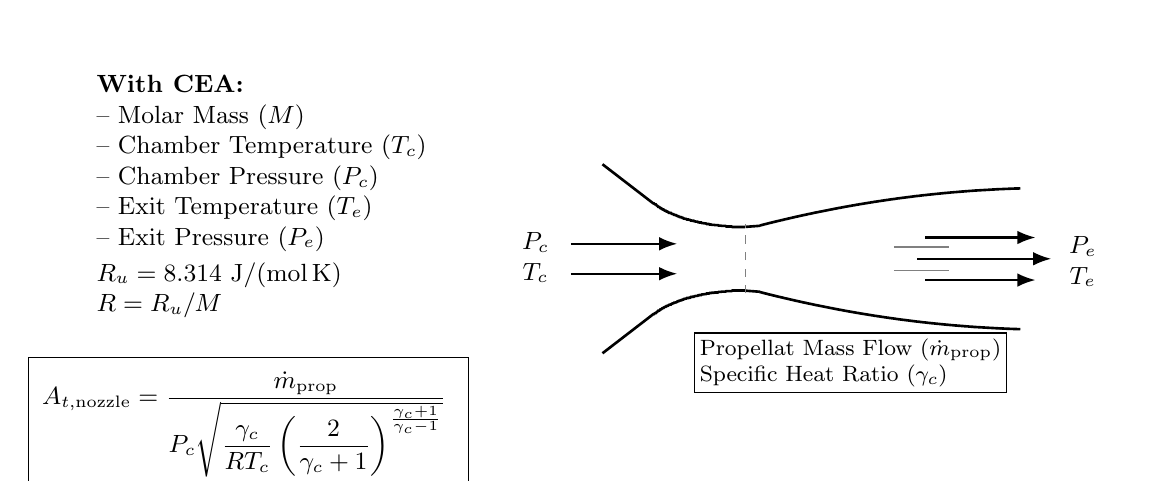
\begin{tikzpicture}[
    >=Latex,
    font=\small,
    station/.style={
        draw,
        rectangle,
        minimum width=2.8cm,
        minimum height=0.9cm,
        align=left,
        fill=white
    },
    box/.style={
        draw,
        rectangle,
        align=left,
        fill=white,
        inner sep=5pt
    },
    flowarrow/.style={
        ->,
        line width=0.8pt
    },
    leader/.style={
        gray,
        line width=0.5pt
    }
]

% =========================================================
% CEA block
% =========================================================
\node[align=left, anchor=north west] (cea) at (-3.0,4.0) {
\textbf{With CEA:}\\
-- Molar Mass $(M)$\\
-- Chamber Temperature $(T_c)$\\
-- Chamber Pressure $(P_c)$\\
-- Exit Temperature $(T_e)$\\
-- Exit Pressure $(P_e)$\\[2pt]
$R_u = 8.314~\mathrm{J/(mol\,K)}$\\
$R = R_u/M$
};

% =========================================================
% Formula block
% =========================================================
\node[box, minimum width=4.6cm, minimum height=1.4cm, anchor=north west] (formula) at (-3.75,0.3) {
$\displaystyle
A_{t,\mathrm{nozzle}}=
\frac{\dot{m}_{\mathrm{prop}}}
{P_c
\sqrt{\dfrac{\gamma_c}{R T_c}
\left(\dfrac{2}{\gamma_c+1}\right)^{\frac{\gamma_c+1}{\gamma_c-1}}}}
$
};

% =========================================================
% Bell-nozzle contour: same piecewise formulation as the 2D plot
% =========================================================

% ----------------------------
% Physical/geometry parameters used only for the schematic contour
% ----------------------------
\pgfmathsetmacro{\rt}{0.020}
\pgfmathsetmacro{\eps}{5.0}
\pgfmathsetmacro{\re}{sqrt(\eps)*\rt}

\pgfmathsetmacro{\alphaDeg}{15}
\pgfmathsetmacro{\bell}{0.80}
\pgfmathsetmacro{\thetaSubDeg}{60}
\pgfmathsetmacro{\thetaInDeg}{30}
\pgfmathsetmacro{\Rch}{0.060}
\pgfmathsetmacro{\tx}{0.055}

% ----------------------------
% Subsonic line and arc
% ----------------------------
\pgfmathsetmacro{\xr}{-1.5*\rt*sin(\thetaSubDeg)}
\pgfmathsetmacro{\yr}{2.5*\rt - 1.5*\rt*cos(\thetaSubDeg)}
\pgfmathsetmacro{\xR}{\tx+\xr}

\pgfmathsetmacro{\mLine}{-tan(\thetaSubDeg)}
\pgfmathsetmacro{\bLine}{\yr - \mLine*\xr}
\pgfmathsetmacro{\xf}{(\Rch - \bLine)/\mLine}
\pgfmathsetmacro{\xF}{\tx+\xf}

% ----------------------------
% Supersonic arc and parabola
% ----------------------------
\pgfmathsetmacro{\rSup}{0.4*\rt}
\pgfmathsetmacro{\Px}{\rSup*sin(\thetaInDeg)}
\pgfmathsetmacro{\Py}{1.4*\rt - \rSup*cos(\thetaInDeg)}
\pgfmathsetmacro{\xP}{\tx+\Px}

\pgfmathsetmacro{\Lcone}{(\re-\rt)/tan(\alphaDeg)}
\pgfmathsetmacro{\L}{\Px + \bell*\Lcone}
\pgfmathsetmacro{\xE}{\tx+\L}

\pgfmathsetmacro{\mZero}{tan(\thetaInDeg)}
\pgfmathsetmacro{\den}{(\L-\Px)}
\pgfmathsetmacro{\aPar}{(\re - \Py - \mZero*(\den))/(\den*\den)}
\pgfmathsetmacro{\bPar}{\mZero - 2*\aPar*\Px}
\pgfmathsetmacro{\cPar}{\Py - \aPar*\Px*\Px - \bPar*\Px}

% ----------------------------
% Drawing transformation
% These values only control the size and position of the schematic
% ----------------------------
\pgfmathsetmacro{\Xstart}{3.55}
\pgfmathsetmacro{\Xscale}{45.0}
\pgfmathsetmacro{\Yaxis}{1.55}
\pgfmathsetmacro{\Rscale}{20}

% Helper idea:
% plotted x = Xstart + Xscale*(x - xF)
% plotted upper y = Yaxis + Rscale*r(x)
% plotted lower y = Yaxis - Rscale*r(x)

% ----------------------------
% Upper wall
% ----------------------------

% 1) initial affine converging line
\draw[line width=0.95pt]
plot[domain=\xF:\xR, samples=2, variable=\x]
(
{\Xstart+\Xscale*(\x-\xF)},
{\Yaxis+\Rscale*(\mLine*(\x-\tx)+\bLine)}
);

% 2) subsonic circular throat arc
\draw[line width=0.95pt]
plot[domain=\xR:\tx, samples=120, variable=\x]
(
{\Xstart+\Xscale*(\x-\xF)},
{\Yaxis+\Rscale*(2.5*\rt - sqrt((1.5*\rt)^2 - (\x-\tx)^2))}
);

% 3) supersonic circular throat arc
\draw[line width=0.95pt]
plot[domain=\tx:\xP, samples=120, variable=\x]
(
{\Xstart+\Xscale*(\x-\xF)},
{\Yaxis+\Rscale*(1.4*\rt - sqrt((0.4*\rt)^2 - (\x-\tx)^2))}
);

% 4) parabolic divergent contour
\draw[line width=0.95pt]
plot[domain=\xP:\xE, samples=220, variable=\x]
(
{\Xstart+\Xscale*(\x-\xF)},
{\Yaxis+\Rscale*(\aPar*(\x-\tx)^2+\bPar*(\x-\tx)+\cPar)}
);

% ----------------------------
% Lower wall: axisymmetric mirror
% ----------------------------

% 1) initial affine converging line
\draw[line width=0.95pt]
plot[domain=\xF:\xR, samples=2, variable=\x]
(
{\Xstart+\Xscale*(\x-\xF)},
{\Yaxis-\Rscale*(\mLine*(\x-\tx)+\bLine)}
);

% 2) subsonic circular throat arc
\draw[line width=0.95pt]
plot[domain=\xR:\tx, samples=120, variable=\x]
(
{\Xstart+\Xscale*(\x-\xF)},
{\Yaxis-\Rscale*(2.5*\rt - sqrt((1.5*\rt)^2 - (\x-\tx)^2))}
);

% 3) supersonic circular throat arc
\draw[line width=0.95pt]
plot[domain=\tx:\xP, samples=120, variable=\x]
(
{\Xstart+\Xscale*(\x-\xF)},
{\Yaxis-\Rscale*(1.4*\rt - sqrt((0.4*\rt)^2 - (\x-\tx)^2))}
);

% 4) parabolic divergent contour
\draw[line width=0.95pt]
plot[domain=\xP:\xE, samples=220, variable=\x]
(
{\Xstart+\Xscale*(\x-\xF)},
{\Yaxis-\Rscale*(\aPar*(\x-\tx)^2+\bPar*(\x-\tx)+\cPar)}
);

% ----------------------------
% Throat marker
% ----------------------------
\draw[dashed, gray]
({\Xstart+\Xscale*(\tx-\xF)},{\Yaxis-\Rscale*\rt-0.04})
--
({\Xstart+\Xscale*(\tx-\xF)},{\Yaxis+\Rscale*\rt+0.04});

% =========================================================
% Station boxes
% =========================================================
\node (p1) at (2.7,1.55) {
\begin{tabular}{c}
$P_c$\\
$T_c$
\end{tabular}
};

\node (p2) at (9.65,1.5) {
\begin{tabular}{c}
$P_e$\\
$T_e$
\end{tabular}
};

% =========================================================
% Mass flow / gamma box
% =========================================================
\node[box,font=\footnotesize,
      minimum width=2.9cm,
      minimum height=0.7cm,
      inner sep=2pt] (massbox) at (6.70,0.23) {
Propellat Mass Flow $(\dot{m}_{\text{prop}})$\\
Specific Heat Ratio $(\gamma_c)$
};

% =========================================================
% Flow arrows
% =========================================================
\draw[flowarrow] (7.55,1.55) -- (9.25,1.55);
\draw[flowarrow] (7.65,1.82) -- (9.05,1.82);
\draw[flowarrow] (7.65,1.28) -- (9.05,1.28);

\draw[flowarrow] (3.15,1.74) -- (4.5,1.74);
\draw[flowarrow] (3.15,1.36) -- (4.5,1.36);

% small flow streak lines
\draw[leader] (7.25,1.70) -- (7.95,1.70);
\draw[leader] (7.25,1.40) -- (7.95,1.40);

\end{tikzpicture}
\caption{Nozzle flow stations used for external throat pre-sizing and ideal one-dimensional analysis.}
\label{fig:flow_stations_tikz}
\end{figure}

\subsubsection{Thrust balance and ideal expansion criterion}

The thrust produced by a rocket nozzle can be approximated by
\begin{equation}
F=\dot{m}V_e+(p_e-p_a)A_e,
\label{eq:thrust}
\end{equation}
where $V_e$ is the exit velocity, $p_e$ is the nozzle exit pressure, $p_a$ is the ambient pressure and $A_e$ is the exit area.

The first term is the momentum thrust. The second term is the pressure thrust. For a fixed chamber condition and mass flow rate, the ideal expansion condition at a given altitude is approximately
\begin{equation}
p_e=p_a .
\label{eq:ideal_expansion}
\end{equation}

When $p_e>p_a$, the nozzle is underexpanded and the gases still have remaining expansion potential at the exit. When $p_e<p_a$, the nozzle is overexpanded, which can lead to compression waves, shocks, separation risk and loss of performance depending on the operating regime.

Because ambient pressure varies during flight, a fixed-geometry nozzle cannot be perfectly expanded at all altitudes. For low-altitude or short-duration flights, the simulator may use a representative ambient pressure, such as sea-level pressure or a trajectory-averaged ambient pressure. For a more complete flight analysis, the expansion ratio should be evaluated over the expected altitude range and the selected value should minimize a trajectory-weighted performance penalty.

\subsubsection{Expansion ratio and exit-plane radius}

The expansion ratio is defined as
\begin{equation}
\varepsilon=\frac{A_e}{A_t} .
\label{eq:expansion_ratio}
\end{equation}

For circular sections,
\begin{equation}
\varepsilon=\frac{\pi r_e^2}{\pi r_t^2}=\left(\frac{r_e}{r_t}\right)^2,
\end{equation}
therefore
\begin{equation}
r_e=\sqrt{\varepsilon}\,r_t .
\label{eq:exit_radius}
\end{equation}

The expansion ratio is one of the most important nozzle design variables. Increasing $\varepsilon$ generally increases exit Mach number and ideal exhaust velocity, but also increases nozzle length, exit area, structural mass and overexpansion risk at low altitude.

\subsubsection{Propellant mass-flow closure from mixture ratio}

Using the conventional definition
\begin{equation}
O/F=\frac{\dot{m}_{ox}}{\dot{m}_{fuel}},
\end{equation}
the fuel mass flow rate is
\begin{equation}
\dot{m}_{fuel}=\frac{\dot{m}_{ox}}{O/F},
\end{equation}
and the total propellant mass flow rate is
\begin{equation}
\dot{m}_{prop}=\dot{m}_{ox}+\dot{m}_{fuel}
=\dot{m}_{ox}\left(1+\frac{1}{O/F}\right).
\label{eq:mdot_total}
\end{equation}

This convention must be used consistently. Reversing the definition of mixture ratio changes the mass-flow calculation and therefore the throat sizing.

% 
% =========================================================

\subsection{Axial flow-field reconstruction}

\subsubsection{Stagnation-to-static isentropic relations}

For one-dimensional, steady, adiabatic and inviscid flow of a perfect gas, the stagnation-to-static relations are
\begin{align}
\frac{T}{T_0} &= \left(1+\frac{\gamma-1}{2}M^2\right)^{-1},
\label{eq:T_T0}\\
\frac{p}{p_0} &= \left(1+\frac{\gamma-1}{2}M^2\right)^{-\gamma/(\gamma-1)},
\label{eq:p_p0}\\
\frac{\rho}{\rho_0} &= \left(1+\frac{\gamma-1}{2}M^2\right)^{-1/(\gamma-1)}.
\label{eq:rho_rho0}
\end{align}

Once the Mach number distribution $M(x)$ is known, these relations provide the axial distributions of temperature, pressure and density.

\subsubsection{Area--Mach compatibility relation}

The Mach number is implicitly related to the local cross-sectional area through the area--Mach relation:
\begin{equation}
\frac{A}{A^*}=\frac{1}{M}
\left[
\frac{2}{\gamma+1}
\left(1+\frac{\gamma-1}{2}M^2\right)
\right]^{\frac{\gamma+1}{2(\gamma-1)}} .
\label{eq:area_mach}
\end{equation}

For a choked nozzle, $A^*=A_t$. Therefore, at each axial station,
\begin{equation}
\frac{A(x)}{A_t}=\frac{\pi r(x)^2}{\pi r_t^2}=\left(\frac{r(x)}{r_t}\right)^2 .
\label{eq:area_ratio_local}
\end{equation}

Equation~\eqref{eq:area_mach} has two possible Mach solutions for $A/A^*>1$: a subsonic solution and a supersonic solution. The correct branch is selected from the location relative to the throat. Upstream of the throat, the subsonic solution is used. Downstream of the throat, the supersonic solution is used. At the throat, $M=1$.

\subsubsection{Branch-resolved numerical solution of the Mach number}

Because Eq.~\eqref{eq:area_mach} cannot generally be inverted explicitly for $M$, the simulator determines $M(x)$ by solving
\begin{equation}
f(M)=\frac{A}{A^*} - \frac{1}{M}
\left[
\frac{2}{\gamma+1}
\left(1+\frac{\gamma-1}{2}M^2\right)
\right]^{\frac{\gamma+1}{2(\gamma-1)}}=0 .
\label{eq:area_mach_residual}
\end{equation}

The implementation uses Brent's bracketed root method, combining the robustness of a bracketing method with faster interpolation steps when the residual permits them. The numerical intervals are
\begin{equation}
M\in(0,1) \quad \text{for the subsonic branch},
\end{equation}
\begin{equation}
M\in(1,M_{max}) \quad \text{for the supersonic branch}.
\end{equation}

Once $M(x)$ is obtained, the local speed of sound and axial velocity are
\begin{equation}
a(x)=\sqrt{\gamma R T(x)},
\end{equation}
\begin{equation}
u(x)=M(x)a(x).
\label{eq:velocity}
\end{equation}


\subsubsection{Axial reconstruction of Mach, static-pressure and static-temperature curves}

The axial property curves couple the piecewise radius function to the
quasi-one-dimensional isentropic model. The process starts from the discretized
nozzle contour,
\begin{equation}
\left\{x_i,r_i\right\}_{i=0}^{N},
\end{equation}
where each station has the local cross-sectional area
\begin{equation}
A_i=\pi r_i^2.
\label{eq:local_area_discrete}
\end{equation}

Because the throat is assumed choked, the critical area is
\begin{equation}
A^*=A_t=\pi r_t^2.
\end{equation}
Therefore, the local area ratio used in the area--Mach equation is
\begin{equation}
\Lambda_i=\frac{A_i}{A_t}=\left(\frac{r_i}{r_t}\right)^2.
\label{eq:local_area_ratio_discrete}
\end{equation}

For each station, the Mach number is obtained by solving the residual form of the area--Mach equation,
\begin{equation}
F(M_i,\Lambda_i)=
\frac{1}{M_i}
\left[
\frac{2}{\gamma+1}
\left(1+\frac{\gamma-1}{2}M_i^2\right)
\right]^{\frac{\gamma+1}{2(\gamma-1)}}
-\Lambda_i=0.
\label{eq:mach_curve_residual}
\end{equation}

The solution branch is selected from the geometric station location:
\begin{equation}
0<M_i<1 \quad \text{for} \quad x_i<x_t,
\end{equation}
\begin{equation}
M_i=1 \quad \text{for} \quad x_i=x_t,
\end{equation}
\begin{equation}
M_i>1 \quad \text{for} \quad x_i>x_t.
\end{equation}
This branch selection is essential because the area--Mach relation is double-valued for \(A/A^*>1\). The same area ratio may correspond either to a subsonic state upstream of the throat or to a supersonic state downstream of it.

After the Mach number has been obtained at each station, the static-temperature curve is generated directly from the stagnation-to-static relation,
\begin{equation}
T_i=T(x_i)=\frac{T_0}{1+\dfrac{\gamma-1}{2}M_i^2}.
\label{eq:temperature_curve}
\end{equation}
Similarly, the static-pressure curve is obtained from
\begin{equation}
p_i=p(x_i)=p_0
\left(1+\frac{\gamma-1}{2}M_i^2\right)^{-\gamma/(\gamma-1)}.
\label{eq:pressure_curve}
\end{equation}
The density curve may also be reconstructed as
\begin{equation}
\rho_i=\rho(x_i)=\rho_0
\left(1+\frac{\gamma-1}{2}M_i^2\right)^{-1/(\gamma-1)}.
\label{eq:density_curve}
\end{equation}

The simulator therefore stores the axial flow-field dataset as
\begin{equation}
\mathcal{D}_{flow}=\left\{x_i,\,A_i,\,\Lambda_i,\,M_i,\,T_i,\,p_i,\,\rho_i,\,u_i\right\}_{i=0}^{N},
\label{eq:flow_dataset}
\end{equation}
where the velocity is obtained from
\begin{equation}
u_i=M_i\sqrt{\gamma R T_i}.
\label{eq:velocity_curve}
\end{equation}

The Mach, pressure and temperature curves are then plotted as functions of the translated axial coordinate \(\bar{x}\). This means that the plotted distributions are not read directly from CEA along the nozzle. CEA/RocketCEA provides the thermochemical closure and reference stagnation properties, while the spatial evolution along the generated contour is reconstructed from \(r(x)\), the area--Mach relation and the isentropic equations.

In the converging subsonic region, reducing area accelerates the flow and increases Mach number toward unity. At the throat, the nozzle becomes choked and $M=1$. In the diverging supersonic region, increasing area further accelerates the flow and produces a supersonic Mach number increase.

The temperature and pressure decrease throughout the expansion according to Eqs.~\eqref{eq:T_T0} and~\eqref{eq:p_p0}. Therefore, the simulator can generate axial distributions of Mach number, pressure and temperature from the geometric contour alone, once the chamber stagnation state and thermodynamic model have been selected.


\newpage
% =========================================================
\section{Axisymmetric Method of Characteristics for
Supersonic Wave Analysis}
\label{sec:moc}
% =========================================================

\subsection{Motivation}

The baseline quasi-one-dimensional model provides a computationally
efficient description of the mean nozzle expansion. However, repeated
optimization runs revealed limitations that are important when the
bell fraction $K_b$ and the initial divergent wall angle
$\theta_{in}$ are treated as design variables.

The main limitations of the quasi-one-dimensional formulation are:

\begin{enumerate}
    \item it cannot resolve the propagation and interaction of
    two-dimensional expansion and compression waves;

    \item it assumes that the flow properties are uniform over each
    cross-section;

    \item it does not resolve the radial distribution of Mach number,
    pressure or flow angle at the nozzle exit;

    \item the axial-momentum loss associated with flow angularity must
    be approximated using an algebraic divergence-efficiency closure;

    \item rapid wall turning and characteristic-wave coalescence are
    not represented explicitly.
\end{enumerate}

These limitations produced the optimization behaviour discussed in
Section~\ref{sec:results}. In particular, the reduced-order model could
prefer very short contours because the viscous wall-friction penalty
was represented, while the possible inviscid benefit of smoother wave
turning and a more uniform exit flow was not resolved.

To establish a direct relationship between $\theta_{in}$, $K_b$ and
the internal supersonic flowfield, an axisymmetric Method of
Characteristics (MOC) solver is introduced. The MOC is used here as a
\emph{prescribed-wall analysis method}: the nozzle contour remains
defined by the parametric geometry model, and the MOC calculates the
flowfield inside that contour.

For each candidate geometry, the required solution variables are

\begin{equation}
    p(x,r), \qquad
    \rho(x,r), \qquad
    V(x,r), \qquad
    M(x,r), \qquad
    T(x,r), \qquad
    \theta(x,r).
\end{equation}

The MOC therefore does not replace the parametric bell-contour model.
Instead, it evaluates the inviscid performance of the contour generated
from the genetic-algorithm variables.

% ---------------------------------------------------------
\subsection{Physical interpretation of the characteristics}
% ---------------------------------------------------------

The Method of Characteristics is derived from the inviscid Euler
equations. In a steady supersonic flow, the governing equations are
hyperbolic. Consequently, information does not propagate arbitrarily
through the domain. Infinitesimal pressure disturbances propagate along
specific directions known as the \emph{characteristics} of the flow.

For a local Mach number $M>1$, the Mach angle is

\begin{equation}
    \boxed{
    \mu =
    \arcsin\left(\frac{1}{M}\right)
    }.
    \label{eq:mach_angle}
\end{equation}

If the local velocity vector forms an angle $\theta$ with the nozzle
axis, the two characteristic directions in the meridional $(x,r)$
plane are

\begin{equation}
    \boxed{
    \frac{dr}{dx}
    =
    \tan(\theta+\mu)
    }
    \qquad \text{along } C^+,
    \label{eq:cplus_direction}
\end{equation}

and

\begin{equation}
    \boxed{
    \frac{dr}{dx}
    =
    \tan(\theta-\mu)
    }
    \qquad \text{along } C^-.
    \label{eq:cminus_direction}
\end{equation}

The streamline is tangent to the local velocity direction $\theta$,
whereas the characteristics are inclined by the Mach angle $\mu$
relative to that streamline. Characteristics should therefore not be
confused with streamlines.

The intersection of one $C^+$ characteristic and one $C^-$
characteristic defines a new solution point. The position of the point
is obtained from the intersection of the characteristic directions,
while the local flow properties are obtained from the corresponding
compatibility equations.


% Replacement for the crowded four-panel Mach-angle/MOC figure.
% Required packages/libraries (already loaded by publication_manuscript/main.tex):
%   pdflscape, caption, tikz
%   \usetikzlibrary{calc,arrows.meta,angles,quotes,positioning}

\clearpage
\begin{landscape}
\thispagestyle{plain}
\vspace{-1cm}
\begin{center}
\begin{minipage}{0.485\linewidth}
\centering
\resizebox{\linewidth}{!}{%
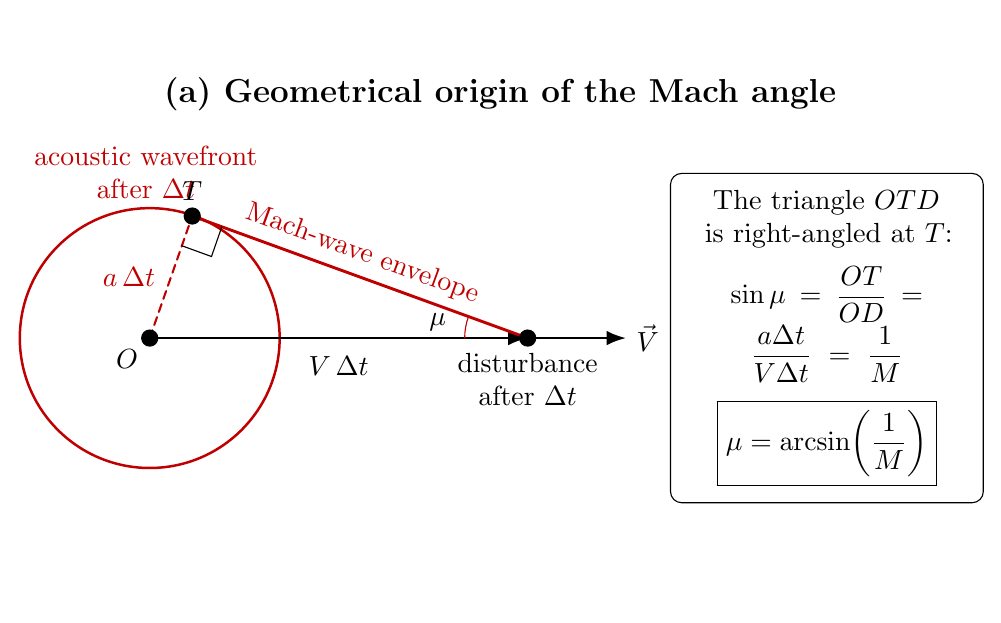
\begin{tikzpicture}[
  line cap=round,
  line join=round,
  >=Latex,
  mainline/.style={black,line width=0.9pt},
  auxiliary/.style={red!75!black,densely dashed,line width=0.75pt},
  characteristic/.style={red!75!black,line width=1.05pt},
  knownpoint/.style={circle,fill=black,inner sep=2.2pt}
]
\path[use as bounding box] (-0.2,-0.2) rectangle (11.8,7.0);

\node[font=\bfseries\large,align=center] at (5.8,6.65)
  {(a) Geometrical origin of the Mach angle};

\coordinate (O) at (1.35,3.55);
\coordinate (D) at (6.15,3.55);
\coordinate (T) at (1.89,5.10);

\draw[red!75!black,line width=0.9pt] (O) circle (1.65);
\node[red!75!black,align=center] at (1.30,5.65)
  {acoustic wavefront\\after $\Delta t$};

\draw[mainline,->] (O) -- (D)
  node[midway,below=3pt] {$V\,\Delta t$};
\draw[auxiliary] (O) -- (T)
  node[midway,left=2pt] {$a\,\Delta t$};
\draw[characteristic] (D) -- (T);
\node[red!75!black,rotate=-20] at (4.05,4.62)
  {Mach-wave envelope};

\node[knownpoint] at (O) {};
\node[knownpoint] at (D) {};
\node[knownpoint] at (T) {};
\node[below left=1pt] at (O) {$O$};
\node[below=2pt,align=center] at (D) {disturbance\\after $\Delta t$};
\node[above=2pt] at (T) {$T$};

\draw[mainline,->] (D) -- ++(1.25,0) node[right] {$\vec V$};
\pic[draw=black,angle radius=4mm] {right angle=D--T--O};
\pic[draw=red!75!black,"$\mu$",angle eccentricity=1.45,
  angle radius=8mm] {angle=T--D--O};

\node[draw=black,rounded corners,align=center,inner sep=6pt,
  text width=3.55cm] at (9.95,3.55)
{
  The triangle $OTD$ is right-angled at $T$:\\[2mm]
  $\displaystyle
    \sin\mu=\frac{OT}{OD}
    =\frac{a\Delta t}{V\Delta t}
    =\frac{1}{M}$
  \\[2mm]
  $\displaystyle
    \boxed{\mu=\arcsin\!\left(\frac{1}{M}\right)}$
};
\end{tikzpicture}%
}
\end{minipage}
\hfill
\begin{minipage}{0.485\linewidth}
\centering
\resizebox{\linewidth}{!}{%
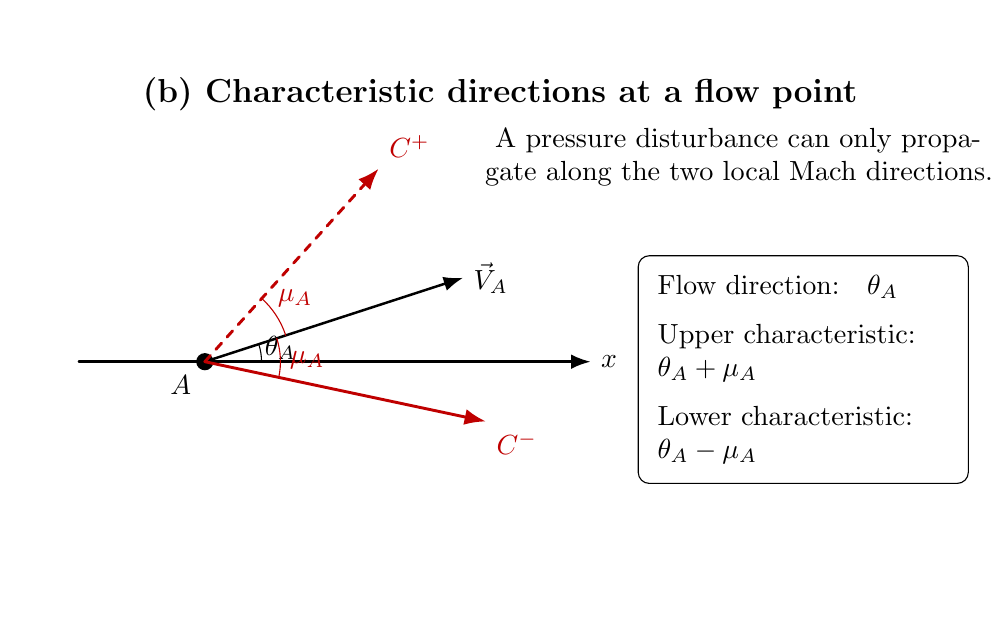
\begin{tikzpicture}[
  line cap=round,
  line join=round,
  >=Latex,
  mainline/.style={black,line width=0.9pt},
  characteristic/.style={red!75!black,line width=1.05pt},
  characteristicplus/.style={red!75!black,dashed,line width=1.05pt},
  knownpoint/.style={circle,fill=black,inner sep=2.2pt}
]
\path[use as bounding box] (-0.2,-0.2) rectangle (11.8,7.0);

\node[font=\bfseries\large,align=center] at (5.8,6.65)
  {(b) Characteristic directions at a flow point};
\node[align=center,text width=10.8cm] at (8.8,5.85)
  {A pressure disturbance can only propagate along the two local Mach directions.};

\coordinate (A) at (2.05,3.25);
\draw[mainline,->] (0.45,3.25) -- (6.95,3.25) node[right] {$x$};
\node[knownpoint] at (A) {};
\node[below left=2pt] at (A) {$A$};

\draw[mainline,->] (A) -- ++(18:3.45) node[right] {$\vec V_A$};
\draw[characteristicplus,->] (A) -- ++(48:3.30)
  node[above right] {$C^+$};
\draw[characteristic,->] (A) -- ++(-12:3.65)
  node[below right] {$C^-$};

\draw[black] ($(A)+(0.72,0)$)
  arc[start angle=0,end angle=18,radius=0.72];
\node at ($(A)+(0.96,0.18)$) {$\theta_A$};

\draw[red!75!black] ($(A)+(18:1.08)$)
  arc[start angle=18,end angle=48,radius=1.08];
\node[red!75!black] at ($(A)+(35:1.40)$) {$\mu_A$};

\draw[red!75!black] ($(A)+(18:0.96)$)
  arc[start angle=18,end angle=-12,radius=0.96];
\node[red!75!black] at ($(A)+(1:1.30)$) {$\mu_A$};

\node[draw=black,rounded corners,align=left,inner sep=7pt,
  text width=3.70cm] at (9.65,3.15)
{
  Flow direction:\quad $\theta_A$\\[2mm]
  Upper characteristic:\quad $\theta_A+\mu_A$\\[2mm]
  Lower characteristic:\quad $\theta_A-\mu_A$
};
\end{tikzpicture}%
}
\end{minipage}

\vspace{0.55cm}

\begin{minipage}{0.485\linewidth}
\centering
\resizebox{\linewidth}{!}{%
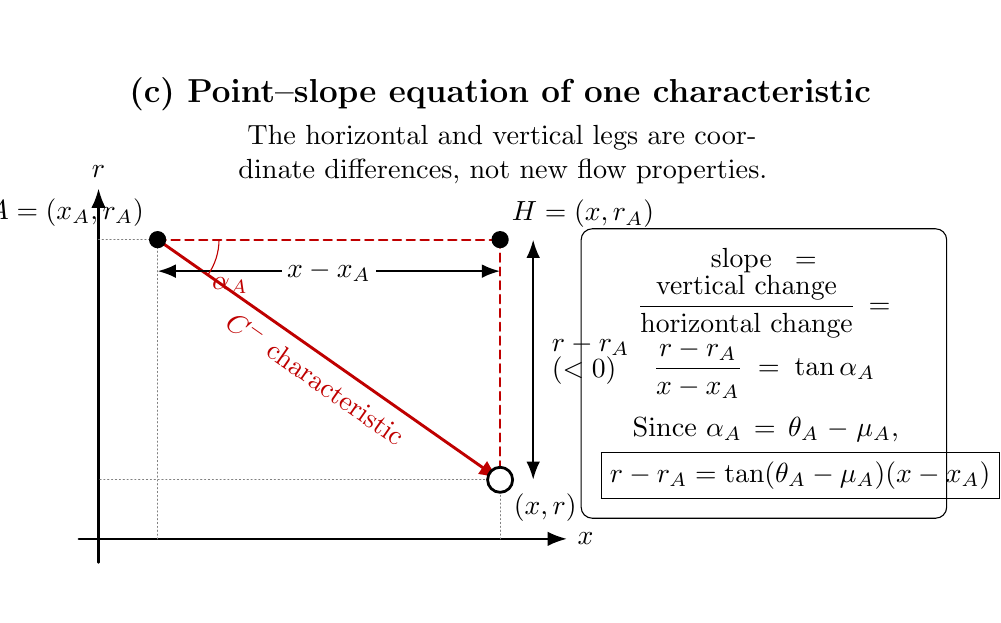
\begin{tikzpicture}[
  line cap=round,
  line join=round,
  >=Latex,
  mainline/.style={black,line width=0.9pt},
  auxiliary/.style={red!75!black,densely dashed,line width=0.75pt},
  characteristic/.style={red!75!black,line width=1.05pt},
  knownpoint/.style={circle,fill=black,inner sep=2.2pt},
  newpoint/.style={circle,draw=black,fill=white,line width=1pt,inner sep=3.2pt}
]
\path[use as bounding box] (-0.2,-0.2) rectangle (11.8,7.0);

\node[font=\bfseries\large,align=center] at (5.8,6.65)
  {(c) Point--slope equation of one characteristic};
\node[align=center,text width=10.8cm] at (5.8,5.88)
  {The horizontal and vertical legs are coordinate differences, not new flow properties.};

\draw[mainline,->] (0.45,1.00) -- (6.65,1.00) node[right] {$x$};
\draw[mainline,->] (0.70,0.70) -- (0.70,5.45) node[above] {$r$};

\coordinate (A) at (1.45,4.80);
\coordinate (P) at (5.80,1.75);
\coordinate (H) at (5.80,4.80);

\draw[characteristic,->] (A) -- (P)
  node[midway,below,sloped] {$C^-$ characteristic};
\draw[auxiliary] (A) -- (H);
\draw[auxiliary] (H) -- (P);

\draw[gray,densely dotted] (A) -- (1.45,1.00);
\draw[gray,densely dotted] (P) -- (5.80,1.00);
\draw[gray,densely dotted] (A) -- (0.70,4.80);
\draw[gray,densely dotted] (P) -- (0.70,1.75);

\node[knownpoint] at (A) {};
\node[newpoint] at (P) {};
\node[knownpoint] at (H) {};
\node[above left=2pt] at (A) {$A=(x_A,r_A)$};
\node[below right=2pt] at (P) {$(x,r)$};
\node[above right=1pt] at (H) {$H=(x,r_A)$};

\draw[<->,black,line width=0.8pt] ($(A)+(0,-0.40)$) --
  ($(H)+(0,-0.40)$)
  node[midway,fill=white,inner sep=2pt] {$x-x_A$};
\draw[<->,black,line width=0.8pt] ($(H)+(0.42,0)$) --
  ($(P)+(0.42,0)$)
  node[midway,right=3pt,align=left] {$r-r_A$\\[-1mm]$(<0)$};

\draw[red!75!black] ($(A)+(0.78,0)$)
  arc[start angle=0,end angle=-35.0,radius=0.78];
\node[red!75!black] at ($(A)+(0.92,-0.58)$) {$\alpha_A$};

\node[draw=black,rounded corners,align=center,inner sep=7pt,
  text width=4.15cm] at (9.15,3.10)
{
  $\displaystyle
  \text{slope}
  =\frac{\text{vertical change}}{\text{horizontal change}}
  =\frac{r-r_A}{x-x_A}
  =\tan\alpha_A$
  \\[2mm]
  Since $\alpha_A=\theta_A-\mu_A$,\\[1mm]
  $\displaystyle
  \boxed{r-r_A=\tan(\theta_A-\mu_A)(x-x_A)}$
};
\end{tikzpicture}%
}
\end{minipage}
\hfill
\begin{minipage}{0.485\linewidth}
\centering
\resizebox{\linewidth}{!}{%
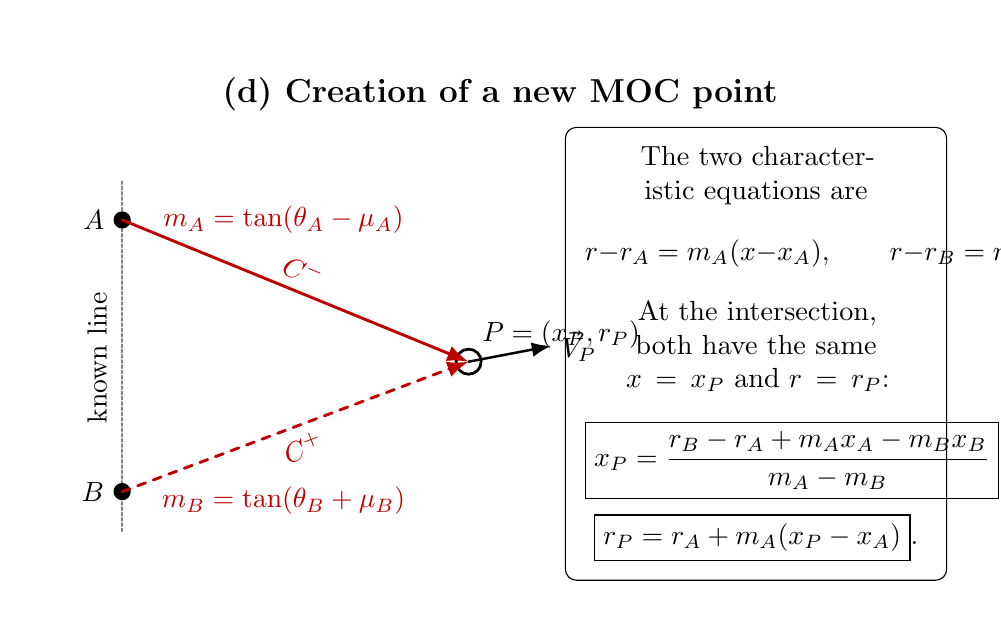
\begin{tikzpicture}[
  line cap=round,
  line join=round,
  >=Latex,
  mainline/.style={black,line width=0.9pt},
  characteristic/.style={red!75!black,line width=1.05pt},
  characteristicplus/.style={red!75!black,dashed,line width=1.05pt},
  knownpoint/.style={circle,fill=black,inner sep=2.2pt},
  newpoint/.style={circle,draw=black,fill=white,line width=1pt,inner sep=3.2pt}
]
\path[use as bounding box] (-0.2,-0.2) rectangle (11.8,7.0);

\node[font=\bfseries\large,align=center] at (5.8,6.65)
  {(d) Creation of a new MOC point};

\draw[gray,densely dotted,line width=0.9pt]
  (1.00,1.10) -- (1.00,5.55);
\node[rotate=90] at (0.68,3.30) {known line};

\coordinate (A) at (1.00,5.05);
\coordinate (B) at (1.00,1.60);
\coordinate (P) at (5.40,3.25);

\node[knownpoint] at (A) {};
\node[knownpoint] at (B) {};
\node[newpoint] at (P) {};
\node[left=3pt] at (A) {$A$};
\node[left=3pt] at (B) {$B$};
\node[above right=2pt] at (P) {$P=(x_P,r_P)$};

\draw[characteristic,->] (A) -- (P)
  node[midway,above,sloped] {$C^-$};
\draw[characteristicplus,->] (B) -- (P)
  node[midway,below,sloped] {$C^+$};
\draw[mainline,->] (P) -- ++(1.05,0.20) node[right] {$\vec V_P$};

\node[red!75!black,align=center] at (3.05,5.05)
  {$m_A=\tan(\theta_A-\mu_A)$};
\node[red!75!black,align=center] at (3.05,1.48)
  {$m_B=\tan(\theta_B+\mu_B)$};

\node[draw=black,rounded corners,align=center,inner sep=7pt,
  text width=4.35cm] at (9.05,3.35)
{
  The two characteristic equations are
  \[
    r-r_A=m_A(x-x_A),\qquad
    r-r_B=m_B(x-x_B).
  \]
  At the intersection, both have the same $x=x_P$ and $r=r_P$:
  \[
    \boxed{x_P=
    \frac{r_B-r_A+m_Ax_A-m_Bx_B}{m_A-m_B}}
  \]
  \vspace{-2mm}
  \[
    \boxed{r_P=r_A+m_A(x_P-x_A)}.
  \]
};
\end{tikzpicture}%
}
\end{minipage}

\vspace{0.35cm}

\captionof{figure}{%
Geometrical interpretation of the Mach angle and construction of a new
Method-of-Characteristics point. 
}
\label{fig:mach_angle_characteristic_geometry}
\end{center}

\end{landscape}
\clearpage
% ---------------------------------------------------------
\subsection{Characteristic compatibility equations}
% ---------------------------------------------------------

The characteristic directions alone determine where information
propagates, but they do not determine how the flow variables change.
The required additional relations are the
\emph{compatibility equations}.

A compatibility equation expresses the combinations of pressure,
velocity and flow angle that must be satisfied between two points
belonging to the same characteristic.

A convenient pressure-based axisymmetric formulation is

\begin{equation}
    Q\,dp+d\theta+S_+\,dx=0
    \qquad \text{along } C^+,
    \label{eq:compatibility_plus}
\end{equation}

and

\begin{equation}
    Q\,dp-d\theta+S_-\,dx=0
    \qquad \text{along } C^-,
    \label{eq:compatibility_minus}
\end{equation}

where

\begin{equation}
    Q
    =
    \frac{\sqrt{M^2-1}}{\rho V^2},
    \label{eq:moc_Q}
\end{equation}

and

\begin{equation}
    S_\pm
    =
    \frac{\sin\theta}
    {rM\cos(\theta\pm\mu)}.
    \label{eq:moc_axisymmetric_source}
\end{equation}

The terms $S_+$ and $S_-$ represent the axisymmetric correction caused
by the changing circumference of the streamtube. They vanish in the
planar-flow limit.

For a planar, isentropic and calorically perfect flow, the compatibility
equations reduce to the familiar Prandtl--Meyer invariants

\begin{equation}
    d(\theta-\nu)=0
    \qquad \text{along } C^+,
\end{equation}

and

\begin{equation}
    d(\theta+\nu)=0
    \qquad \text{along } C^-,
\end{equation}

where $\nu=\nu(M)$ is the Prandtl--Meyer function:
\begin{equation}
\nu(M)
=
\sqrt{\frac{\gamma+1}{\gamma-1}}
\tan^{-1}
\left[
\sqrt{
\frac{\gamma-1}{\gamma+1}
\left(M^2-1\right)
}
\right]
-
\tan^{-1}
\left(
\sqrt{M^2-1}
\right).
\label{eq:prandtl_meyer}
\end{equation}
In the axisymmetric formulation these quantities are no longer exactly
constant, and the geometric source terms must be integrated numerically
along each characteristic segment.

The sign convention used in
Equations~\eqref{eq:cplus_direction}--\eqref{eq:compatibility_minus}
must remain consistent throughout the implementation. Alternative
references may interchange the names $C^+$ and $C^-$.

% ---------------------------------------------------------
\subsection{Characteristic mesh and numerical marching}
% ---------------------------------------------------------

The MOC does not use a conventional rectangular computational grid.
Instead, the numerical mesh is generated by the intersections of the
$C^+$ and $C^-$ characteristic families.

The solution begins from a transonic initial line located immediately
downstream of the geometric . This line contains a discrete
distribution of the form

\begin{equation}
    \left\{
    x_i,\,
    r_i,\,
    p_i,\,
    \rho_i,\,
    V_i,\,
    M_i,\,
    \theta_i
    \right\},
    \qquad i=1,\ldots,N.
\end{equation}

Because the characteristic equations become degenerate at $M=1$, a
uniform sonic line cannot be used directly. The initial data should be
obtained from an axisymmetric transonic throat solution based on the
local throat curvature.

For an interior point $P$, one $C^+$ characteristic is traced from a
known point $A$ and one $C^-$ characteristic from a known point $B$.
Their approximate intersection provides the new coordinates
$(x_P,r_P)$. The two compatibility equations then provide the local
pressure and flow angle.

Since the characteristic slopes depend on the unknown properties at
$P$, the solution is obtained using a predictor--corrector procedure:

\begin{enumerate}
    \item calculate a first estimate using the properties at $A$ and
    $B$;

    \item evaluate the predicted properties at $P$;

    \item recompute the characteristic slopes using averaged properties;

    \item repeat until the changes in position and flow properties fall
    below the prescribed convergence tolerance.
\end{enumerate}

Interpolation is required whenever the foot of a new characteristic
falls between two nodes of the previous characteristic line. The resulting characteristic mesh and the local construction of an
interior solution point are illustrated schematically in
Figure~\ref{fig:prescribed_wall_moc_mesh}.

\begin{figure}[htbp]
\centering

% =========================================================
% (a) Global characteristic mesh
% =========================================================

\resizebox{0.98\textwidth}{!}{%
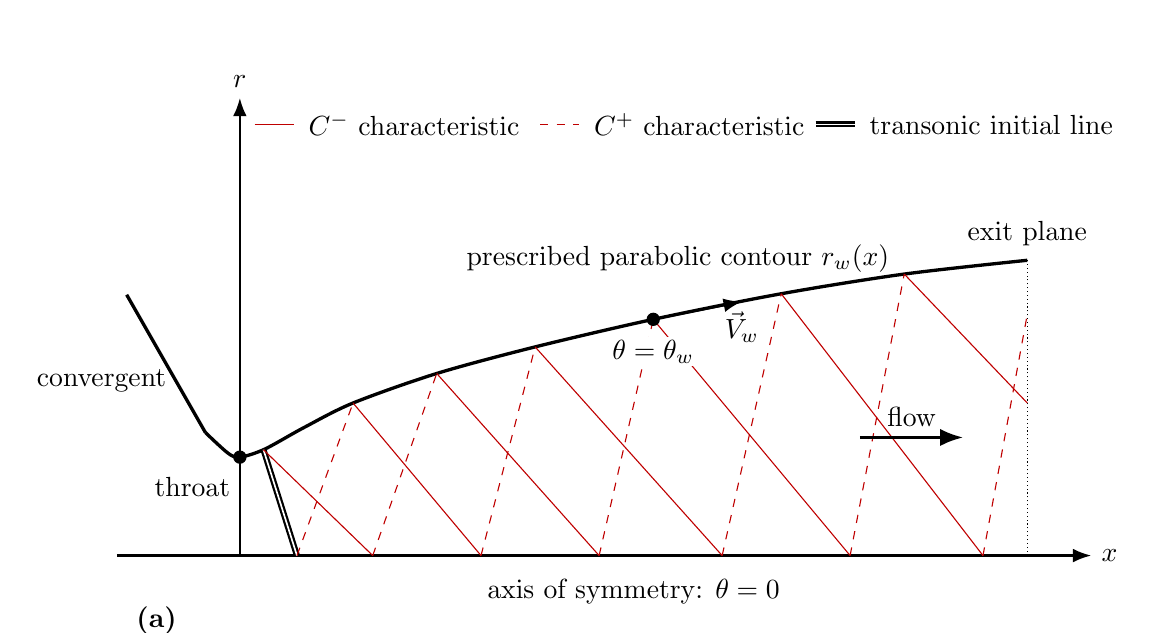
\begin{tikzpicture}[
    x=1.25cm,
    y=1.25cm,
    >=Latex,
    wall/.style={very thick,draw=black},
    axisline/.style={thick,draw=black},
    cplus/.style={thin,dashed,draw=red!75!black},
    cminus/.style={thin,draw=red!75!black},
    initial/.style={thick,double,draw=black},
    point/.style={circle,fill=black,inner sep=1.7pt}
]

% ---------------------------------------------------------
% Coordinate system
% ---------------------------------------------------------

\draw[axisline,->]
    (-1.25,0) -- (8.65,0)
    node[right] {$x$};

\draw[axisline,->]
    (0,0) -- (0,4.65)
    node[above] {$r$};

\node[below] at (4.0,-0.14)
    {axis of symmetry: $\theta=0$};

% ---------------------------------------------------------
% Prescribed nozzle wall
% ---------------------------------------------------------

% Convergent section
\draw[wall]
    (-1.15,2.65)
    --
    (-0.35,1.25);

% Throat arc and bell contour
\draw[wall]
    plot[smooth] coordinates {
        (-0.35,1.25)
        (-0.12,1.04)
        ( 0.00,1.00)
        ( 0.25,1.08)
        ( 0.65,1.30)
        ( 1.15,1.55)
        ( 2.00,1.85)
        ( 3.00,2.12)
        ( 4.20,2.40)
        ( 5.50,2.66)
        ( 6.75,2.86)
        ( 8.00,3.00)
    };

\node[above left] at (-0.65,1.56)
    {convergent};

\node[above] at (4.45,2.78)
    {prescribed parabolic contour $r_w(x)$};

% ---------------------------------------------------------
% Throat and exit
% ---------------------------------------------------------

\draw[densely dotted]
    (0,0) -- (0,1.00);

\node[point] at (0,1.00) {};
\node[above left] at (0,0.500)
    {throat};

\draw[densely dotted]
    (8.00,0) -- (8.00,3.00);

\node[above] at (8.00,3.05)
    {exit plane};

% ---------------------------------------------------------
% Initial transonic line
% ---------------------------------------------------------

\draw[initial]
    (0.24,1.075) -- (0.58,0);


% ---------------------------------------------------------
% C-minus characteristics
% Solid red lines: wall towards axis
% ---------------------------------------------------------

\draw[cminus]
    (0.24,1.075) -- (1.35,0);

\draw[cminus]
    (1.15,1.55) -- (2.45,0);

\draw[cminus]
    (2.00,1.85) -- (3.65,0);

\draw[cminus]
    (3.00,2.12) -- (4.90,0);

\draw[cminus]
    (4.20,2.40) -- (6.20,0);

\draw[cminus]
    (5.50,2.66) -- (7.55,0);

\draw[cminus]
    (6.75,2.86) -- (8.00,1.55);

% ---------------------------------------------------------
% C-plus characteristics
% Dashed red lines: axis towards wall
% ---------------------------------------------------------

\draw[cplus]
    (0.58,0) -- (1.15,1.55);

\draw[cplus]
    (1.35,0) -- (2.00,1.85);

\draw[cplus]
    (2.45,0) -- (3.00,2.12);

\draw[cplus]
    (3.65,0) -- (4.20,2.40);

\draw[cplus]
    (4.90,0) -- (5.50,2.66);

\draw[cplus]
    (6.20,0) -- (6.75,2.86);

\draw[cplus]
    (7.55,0) -- (8.00,2.45);

% ---------------------------------------------------------
% Wall tangency
% ---------------------------------------------------------

\node[point] (W) at (4.20,2.40) {};

\draw[->,thick]
    (W) -- ++(0.90,0.18)
    node[below] {$\vec V_w$};

\node[
    fill=white,
    inner sep=1pt
] at (4.2,2.07)
    {$\theta=\theta_w$};

% ---------------------------------------------------------
% Flow direction
% ---------------------------------------------------------

\draw[->,very thick]
    (6.30,1.20) -- (7.35,1.20)
    node[midway,above] {flow};

% ---------------------------------------------------------
% Legend
% ---------------------------------------------------------

\begin{scope}[shift={(0.15,3.38)}]

    \draw[cminus]
        (0,1) -- (0.40,1);

    \node[right] at (0.45,1)
        {$C^-$ characteristic};

    \draw[cplus]
        (2.90,1) -- (3.30,1);

    \node[right] at (3.35,1)
        {$C^+$ characteristic};

    \draw[initial]
        (5.70,1) -- (6.10,1);
        
    \node[right] at (6.15,1)
        {transonic initial line};
\end{scope}

% Panel identifier
\node[anchor=north west,font=\bfseries]
    at (-1.15,-0.42) {(a)};

\end{tikzpicture}%
}

\vspace{0.7cm}

% =========================================================
% (b) Close-up of one characteristic intersection
% =========================================================

\resizebox{0.76\textwidth}{!}{%
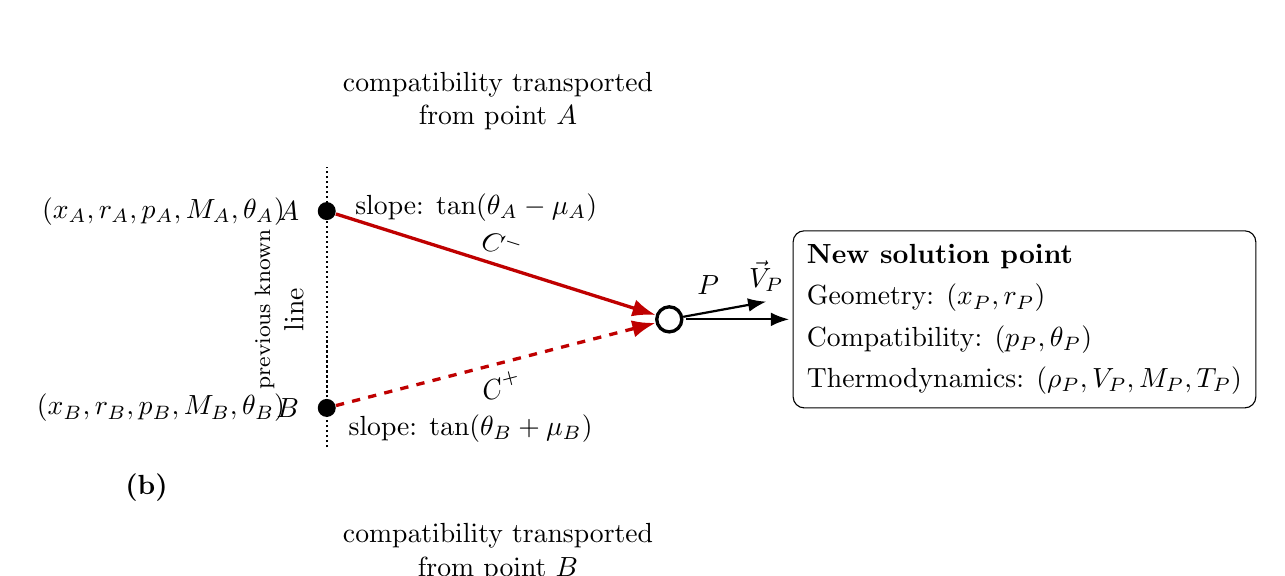
\begin{tikzpicture}[
    x=1.45cm,
    y=1.25cm,
    >=Latex,
    cplus/.style={very thick,dashed,draw=red!75!black},
    cminus/.style={very thick,draw=red!75!black},
    knownpoint/.style={
        circle,
        fill=black,
        inner sep=2.3pt
    },
    newpoint/.style={
        circle,
        draw=black,
        very thick,
        fill=white,
        inner sep=3.2pt
    }
]

% ---------------------------------------------------------
% Previous characteristic/data line
% ---------------------------------------------------------

\draw[thick,densely dotted]
    (0,0.35) -- (0,3.20);

\node[
    rotate=90,
    above,
    align=center
]
at (-0.12,1.75)
{\footnotesize previous known\\line};

% ---------------------------------------------------------
% Known points A and B
% ---------------------------------------------------------

\node[knownpoint] (A) at (0,2.75) {};
\node[left=3pt of A]
    {$A$};

\node[knownpoint] (B) at (0,0.75) {};
\node[left=3pt of B]
    {$B$};

\node[align=right,anchor=east]
    at (-0.20,2.75)
{
$\left(x_A,r_A,p_A,M_A,\theta_A\right)$
};

\node[align=right,anchor=east]
    at (-0.20,0.75)
{
$\left(x_B,r_B,p_B,M_B,\theta_B\right)$
};

% ---------------------------------------------------------
% New point P
% ---------------------------------------------------------

\node[newpoint] (P) at (3.00,1.65) {};

\node[above right=2pt and 3pt of P]
    {$P$};

% C-minus from A
\draw[cminus,->]
    (A) -- (P)
    node[midway,above,sloped]
    {$C^-$};

% C-plus from B
\draw[cplus,->]
    (B) -- (P)
    node[midway,below,sloped]
    {$C^+$};

% ---------------------------------------------------------
% Local characteristic directions
% ---------------------------------------------------------

\node[
    align=center,
    anchor=south
] at (1.35,2.55)
{
slope:
$\tan(\theta_A-\mu_A)$
};

\node[
    align=center,
    anchor=north
] at (1.30,0.78)
{
slope:
$\tan(\theta_B+\mu_B)$
};

% ---------------------------------------------------------
% State calculation at P
% ---------------------------------------------------------

\draw[->,thick]
    (3.15,1.65) -- (4.05,1.65);

\node[
    draw=black,
    rounded corners,
    align=left,
    anchor=west,
    inner sep=5pt
] at (4.08,1.65)
{
\textbf{New solution point}\\[1mm]
Geometry:
$(x_P,r_P)$\\[1mm]
Compatibility:
$(p_P,\theta_P)$\\[1mm]
Thermodynamics:
$(\rho_P,V_P,M_P,T_P)$
};

% ---------------------------------------------------------
% Compatibility labels
% ---------------------------------------------------------

\node[
    align=center,
    fill=white,
    inner sep=2pt
] at (1.500,3.87)
{
compatibility transported\\
from point $A$
};

\node[
    align=center,
    fill=white,
    inner sep=2pt
] at (1.500,-0.72)
{
compatibility transported\\
from point $B$
};

% ---------------------------------------------------------
% Flow vector at P
% ---------------------------------------------------------

\draw[->,thick]
    (P) -- ++(0.85,0.18)
    node[above] {$\vec V_P$};

% Panel identifier
\node[anchor=north west,font=\bfseries]
    at (-1.85,0.18) {(b)};

\end{tikzpicture}%
}

\caption{
Schematic representation of the axisymmetric Method of
Characteristics used for prescribed-wall nozzle analysis.
(a) Characteristic mesh inside the parametric bell-nozzle contour.
The solid and dashed red lines represent the $C^-$ and $C^+$
characteristic families, respectively.
(b) Local construction of a new interior point $P$ from the
intersection of two characteristics originating from the known
points $A$ and $B$.
}

\label{fig:prescribed_wall_moc_mesh}

\end{figure}

As shown in Figure~\ref{fig:prescribed_wall_moc_mesh}(b), the
coordinates $(x_P,r_P)$ are obtained from the intersection of the
two characteristic directions. The local pressure and flow angle are
then determined from the two compatibility equations. The remaining
thermodynamic properties follow from the energy equation and the
selected gas model.

At the nozzle wall, the flow-tangency boundary condition is

\begin{equation}
    \boxed{
    \theta_w
    =
    \arctan\left(\frac{dr_w}{dx}\right)
    }.
    \label{eq:moc_wall_condition}
\end{equation}

At the axis of symmetry,

\begin{equation}
    \boxed{
    r=0,
    \qquad
    \theta=0
    }.
    \label{eq:moc_axis_condition}
\end{equation}

The $1/r$ dependence of the axisymmetric source term requires a
dedicated limiting formulation at the axis. Direct evaluation of
Equation~\eqref{eq:moc_axisymmetric_source} at $r=0$ is not permitted.

The resulting characteristic mesh is illustrated in
Figure~\ref{fig:prescribed_wall_moc_mesh}.

% Insert the monochromatic TikZ figure here.


\subsection{Axis-of-symmetry limiting treatment}
\label{sec:moc_axis_treatment}

The axis of symmetry requires a dedicated boundary formulation. The
axisymmetric compatibility source terms,

\begin{equation}
S^\pm =
\frac{\sin\theta}
{rM\cos(\theta\pm\mu)},
\label{eq:moc_axisymmetric_source_recalled}
\end{equation}

cannot be evaluated directly at \(r=0\), because the symmetry condition
also imposes \(\theta=0\). Direct substitution would therefore produce
the indeterminate form \(0/0\). This is a coordinate singularity rather
than a physical singularity, and its finite limit follows from the
regularity and parity of the flow variables near the axis.

\subsubsection{Parity of the flow variables}

To examine the local behaviour around the axis, the radial coordinate
may temporarily be extended to a signed coordinate. Reflection across
the axis corresponds to

\begin{equation}
r\longrightarrow-r.
\end{equation}

The scalar flow properties are unchanged by this reflection:

\begin{equation}
p(x,-r)=p(x,r),
\qquad
\rho(x,-r)=\rho(x,r),
\end{equation}

\begin{equation}
T(x,-r)=T(x,r),
\qquad
M(x,-r)=M(x,r).
\end{equation}

The axial velocity component \(u\) is also unchanged,

\begin{equation}
u(x,-r)=u(x,r),
\end{equation}

whereas the radial velocity component \(v\) reverses direction:

\begin{equation}
v(x,-r)=-v(x,r).
\end{equation}

Consequently, \(u\) is locally an even function of \(r\), while \(v\)
is locally an odd function. For a smooth solution, their Taylor
expansions near \(r=0\) are therefore

\begin{equation}
u(x,r)
=
u_0(x)+u_2(x)r^2
+\mathcal{O}(r^4),
\label{eq:axis_u_expansion}
\end{equation}

and

\begin{equation}
v(x,r)
=
v_1(x)r+v_3(x)r^3
+\mathcal{O}(r^5).
\label{eq:axis_v_expansion}
\end{equation}

Since the local flow angle is defined by

\begin{equation}
\theta(x,r)
=
\tan^{-1}
\left(
\frac{v(x,r)}{u(x,r)}
\right),
\label{eq:flow_angle_velocity_definition}
\end{equation}

it is also an odd function of the radial coordinate:

\begin{equation}
\theta(x,-r)=-\theta(x,r).
\end{equation}

Its local Taylor expansion consequently contains only odd powers:

\begin{equation}
\boxed{
\theta(x,r)
=
c_1(x)r+c_3(x)r^3
+\mathcal{O}(r^5)
}.
\label{eq:axis_theta_expansion}
\end{equation}

The coefficients in Equation~\eqref{eq:axis_theta_expansion} are not
empirical loss coefficients. They are local derivatives of the
axisymmetric flowfield. In particular,

\begin{equation}
\boxed{
c_1(x)
=
\left.
\frac{\partial\theta}{\partial r}
\right|_{r=0}
}.
\label{eq:c1_axis_derivative}
\end{equation}

Expanding Equation~\eqref{eq:flow_angle_velocity_definition} using
Equations~\eqref{eq:axis_u_expansion} and
\eqref{eq:axis_v_expansion} gives

\begin{equation}
c_1(x)=\frac{v_1(x)}{u_0(x)},
\end{equation}

and

\begin{equation}
c_3(x)
=
\frac{v_3(x)}{u_0(x)}
-
\frac{v_1(x)u_2(x)}{u_0(x)^2}
-
\frac{1}{3}
\left(
\frac{v_1(x)}{u_0(x)}
\right)^3.
\end{equation}

Equation~\eqref{eq:axis_theta_expansion} is only a local expansion
around the axis. It does not assume that the complete radial flow-angle
distribution is a cubic polynomial.

\subsubsection{Finite limit of the axisymmetric source term}

Using Equation~\eqref{eq:axis_theta_expansion}, the flow angle close to
the axis satisfies

\begin{equation}
\sin\theta
=
c_1r+\mathcal{O}(r^3).
\end{equation}

It follows that

\begin{equation}
\lim_{r\rightarrow0}
\frac{\sin\theta}{r}
=
c_1
=
\left.
\frac{\partial\theta}{\partial r}
\right|_{r=0}.
\label{eq:sin_theta_over_r_limit}
\end{equation}

At the axis, \(\theta=0\), and therefore

\begin{equation}
\cos(\theta\pm\mu)
\longrightarrow
\cos(\pm\mu)
=
\cos\mu.
\end{equation}

The limiting value of Equation~
\eqref{eq:moc_axisymmetric_source_recalled} is consequently

\begin{equation}
\boxed{
S^\pm_{\mathrm{axis}}
=
\frac{1}
{M_{\mathrm{axis}}\cos\mu_{\mathrm{axis}}}
\left.
\frac{\partial\theta}{\partial r}
\right|_{r=0}
}.
\label{eq:S_axis_first_form}
\end{equation}

Since

\begin{equation}
\sin\mu_{\mathrm{axis}}
=
\frac{1}{M_{\mathrm{axis}}},
\end{equation}

then

\begin{equation}
M_{\mathrm{axis}}\cos\mu_{\mathrm{axis}}
=
\sqrt{M_{\mathrm{axis}}^2-1}.
\end{equation}

The axis limit can therefore also be written as

\begin{equation}
\boxed{
S^\pm_{\mathrm{axis}}
=
\frac{1}
{\sqrt{M_{\mathrm{axis}}^2-1}}
\left.
\frac{\partial\theta}{\partial r}
\right|_{r=0}
}.
\label{eq:S_axis_final}
\end{equation}

The two characteristic families have the same limiting source term at
the axis because

\begin{equation}
\cos(+\mu_{\mathrm{axis}})
=
\cos(-\mu_{\mathrm{axis}}).
\end{equation}

No artificial minimum radius is therefore required. Replacing \(r\)
with \(\max(r,\varepsilon_r)\) would alter the compatibility equations
and conceal the coordinate singularity instead of resolving it.

\subsubsection{Construction of a characteristic point on the axis}

Consider a known interior point

\begin{equation}
A=
\left(
x_A,r_A,p_A,M_A,\theta_A
\right),
\qquad r_A>0,
\end{equation}

from which a \(C^-\) characteristic reaches the axis at the new point

\begin{equation}
P=
\left(
x_P,0,p_P,M_P,0
\right).
\end{equation}

The axis conditions provide

\begin{equation}
\boxed{
r_P=0,
\qquad
\theta_P=0
}.
\label{eq:moc_axis_conditions}
\end{equation}

The \(C^-\) characteristic direction is

\begin{equation}
\frac{dr}{dx}
=
\tan(\theta-\mu).
\end{equation}

Using the properties at \(A\) as a first-order geometrical predictor,

\begin{equation}
-r_A
=
(x_P-x_A)
\tan(\theta_A-\mu_A),
\end{equation}

which gives

\begin{equation}
\boxed{
x_P
=
x_A
-
\frac{r_A}
{\tan(\theta_A-\mu_A)}
}.
\label{eq:axis_point_predictor}
\end{equation}

The pressure-based \(C^-\) compatibility equation is

\begin{equation}
Q\,dp-d\theta+S^-\,dx=0.
\label{eq:Cminus_axis_compatibility}
\end{equation}

A second-order finite-difference approximation between \(A\) and \(P\)
is

\begin{equation}
\overline{Q}_{AP}(p_P-p_A)
-
(\theta_P-\theta_A)
+
\overline{S^-}_{AP}(x_P-x_A)
=
0,
\label{eq:axis_discrete_compatibility}
\end{equation}

where

\begin{equation}
\overline{Q}_{AP}
=
\frac{Q_A+Q_P}{2},
\end{equation}

and

\begin{equation}
\overline{S^-}_{AP}
=
\frac{S^-_A+S^-_{\mathrm{axis}}}{2}.
\end{equation}

Using \(\theta_P=0\), the axis pressure is obtained from

\begin{equation}
\boxed{
p_P
=
p_A
-
\frac{
\theta_A+
\overline{S^-}_{AP}(x_P-x_A)
}{
\overline{Q}_{AP}
}
}.
\label{eq:axis_pressure_update}
\end{equation}

Because \(Q_P\), \(S^-_{\mathrm{axis}}\), \(\mu_P\) and the corrected
characteristic slope depend on the initially unknown state at \(P\),
Equations~\eqref{eq:axis_point_predictor}--
\eqref{eq:axis_pressure_update} are solved using the same
predictor--corrector strategy employed for an interior characteristic
point:

\begin{enumerate}
    \item predict \(x_P\) using the properties at \(A\);
    \item impose \(r_P=0\) and \(\theta_P=0\);
    \item predict \(p_P\) from the \(C^-\) compatibility equation;
    \item calculate the remaining thermodynamic properties and obtain
    \(M_P\) and \(\mu_P\);
    \item evaluate the limiting source
    \(S^-_{\mathrm{axis}}\);
    \item recompute the characteristic geometry and averaged
    compatibility coefficients;
    \item repeat until both the position and flow properties converge.
\end{enumerate}

For the corrected geometry, the characteristic slope is averaged
between \(A\) and \(P\):

\begin{equation}
-r_A
=
\frac{x_P-x_A}{2}
\left[
\tan(\theta_A-\mu_A)
+
\tan(\theta_P-\mu_P)
\right].
\end{equation}

Since \(\theta_P=0\),

\begin{equation}
\boxed{
-r_A
=
\frac{x_P-x_A}{2}
\left[
\tan(\theta_A-\mu_A)
-
\tan\mu_P
\right]
}.
\label{eq:axis_corrected_geometry}
\end{equation}

\subsubsection{Numerical estimation of the axis derivative}

The derivative required by Equation~\eqref{eq:S_axis_final} should be
estimated from interior points at the same axial characteristic station
as the new axis point. Using the closest interior point \(Q_1\),

\begin{equation}
\left.
\frac{\partial\theta}{\partial r}
\right|_{r=0}
\approx
\frac{\theta_{Q_1}}{r_{Q_1}},
\label{eq:axis_derivative_first_order}
\end{equation}

provides a first-order estimate.

A higher-order estimate can be obtained from two interior points
\(Q_1\) and \(Q_2\) by fitting the symmetry-preserving expansion

\begin{equation}
\theta(r)=c_1r+c_3r^3.
\end{equation}

The coefficients satisfy

\begin{equation}
\begin{bmatrix}
r_{Q_1} & r_{Q_1}^3\\
r_{Q_2} & r_{Q_2}^3
\end{bmatrix}
\begin{bmatrix}
c_1\\
c_3
\end{bmatrix}
=
\begin{bmatrix}
\theta_{Q_1}\\
\theta_{Q_2}
\end{bmatrix}.
\label{eq:axis_odd_polynomial_fit}
\end{equation}

The required axis derivative is then

\begin{equation}
\boxed{
\left.
\frac{\partial\theta}{\partial r}
\right|_{r=0}
=
c_1
=
\frac{
r_{Q_2}^{\,2}\theta_{Q_1}/r_{Q_1}
-
r_{Q_1}^{\,2}\theta_{Q_2}/r_{Q_2}
}{
r_{Q_2}^{\,2}-r_{Q_1}^{\,2}
}
}.
\label{eq:axis_derivative_second_order}
\end{equation}

Using a point located at a different axial coordinate, such as the
incoming characteristic point \(A\), through the approximation
\(\theta_A/r_A\), is acceptable only as an initial predictor. The
converged axis derivative should be obtained from points belonging to
the same downstream characteristic station.
% ---------------------------------------------------------
\subsection{Exit-plane thrust integration}
% ---------------------------------------------------------

The MOC provides a non-uniform radial flow profile at the nozzle exit.
The local axial velocity is

\begin{equation}
    u_e(r)=V_e(r)\cos\theta_e(r).
\end{equation}

The exit mass flow rate is evaluated from

\begin{equation}
    \boxed{
    \dot{m}_e
    =
    2\pi
    \int_0^{R_e}
    \rho_e(r)u_e(r)\,r\,dr
    }.
    \label{eq:moc_exit_massflow}
\end{equation}

The inviscid thrust is

\begin{equation}
    \boxed{
    F_{\mathrm{MOC}}
    =
    2\pi
    \int_0^{R_e}
    \left[
        \rho_e(r)u_e^2(r)
        +
        p_e(r)-p_a
    \right]r\,dr
    }.
    \label{eq:moc_thrust}
\end{equation}

The corresponding inviscid thrust coefficient is

\begin{equation}
    \boxed{
    C_{F,\mathrm{MOC}}
    =
    \frac{F_{\mathrm{MOC}}}{p_cA_t}
    }.
    \label{eq:moc_thrust_coefficient}
\end{equation}

Because the local velocity direction is resolved over the complete exit
plane, the axial-momentum effect of flow divergence is already included
in Equation~\eqref{eq:moc_thrust}. Consequently, a separate algebraic
factor such as $\eta_{div}=\cos\theta_{out}$ is not required in the
MOC-based evaluation.

% ---------------------------------------------------------
\subsection{Coupling with the boundary-layer model}
% ---------------------------------------------------------

The inviscid MOC solution supplies the boundary-layer edge conditions

\begin{equation}
    p_e(x),\qquad
    T_e(x),\qquad
    \rho_e(x),\qquad
    V_e(x),\qquad
    M_e(x)
\end{equation}

along the nozzle wall. These quantities are passed to the integral
boundary-layer model, which calculates

\begin{equation}
    \tau_w(x),\qquad
    C_f(x),\qquad
    \delta^*(x).
\end{equation}

The axial wall-friction force is

\begin{equation}
    \boxed{
    F_f
    =
    2\pi
    \int_{x_t}^{x_e}
    \tau_w(x)r_w(x)\,dx
    }.
    \label{eq:moc_wall_friction}
\end{equation}

The loss-corrected thrust coefficient is therefore

\begin{equation}
    \boxed{
    C_{F,\mathrm{eff}}
    =
    \frac{F_{\mathrm{MOC}}-F_f}{p_cA_t}
    }.
    \label{eq:moc_effective_cf}
\end{equation}

Boundary-layer separation is not predicted by the inviscid MOC itself.
Instead, the MOC provides the wall-pressure distribution and adverse
pressure gradient required by the boundary-layer model. Separation is
identified when the calculated wall shear stress approaches zero and
changes sign,

\begin{equation}
    \tau_w \rightarrow 0,
\end{equation}

followed by

\begin{equation}
    \tau_w<0.
\end{equation}

% ---------------------------------------------------------
\subsection{Shock detection and present limitations}
% ---------------------------------------------------------

The present MOC formulation assumes a continuous and shock-free
supersonic flowfield. Compression characteristics may converge and
eventually intersect. Such characteristic coalescence indicates that a
smooth isentropic solution no longer exists and that a shock may form.

Until a dedicated shock-fitting method is implemented, characteristic
intersection is treated as a solver-failure condition rather than as a
calculated post-shock solution. Therefore, the present model resolves
smooth expansion and compression waves, but it does not yet calculate
the downstream state across a finite-strength shock.

The main assumptions of the present formulation are:

\begin{enumerate}
    \item steady axisymmetric flow;

    \item inviscid core flow;

    \item no swirl;

    \item calorically perfect gas in the first implementation;

    \item smooth supersonic solution without fitted shocks;

    \item boundary-layer effects treated through a separate integral
    model.
\end{enumerate}

% ---------------------------------------------------------
\subsection{Numerical verification}
% ---------------------------------------------------------

Mass-flow conservation is used as a primary numerical diagnostic. The
relative mass-flow residual is

\begin{equation}
    \boxed{
    \varepsilon_{\dot m}
    =
    \left|
    \frac{\dot m_e-\dot m_t}{\dot m_t}
    \right|
    }.
    \label{eq:moc_mass_residual}
\end{equation}

A solution is accepted for optimization only when the mass-flow
residual, local predictor--corrector residuals and mesh-quality criteria
remain below their prescribed tolerances.

Grid convergence is evaluated by successively refining both the initial
characteristic line and the prescribed wall discretization. The
quantities monitored during refinement include

\begin{equation}
    \dot m_e,\qquad
    C_{F,\mathrm{MOC}},\qquad
    p_e(r),\qquad
    M_e(r),\qquad
    \theta_e(r).
\end{equation}



\newpage
\section{Kliegel--Levine Axisymmetric Transonic Initial-Line Model}
\label{sec:kliegel_levine_initial_line}
% =========================================================

\subsection{Purpose of the model}

The Kliegel--Levine model supplies a local analytical approximation to the
axisymmetric flow field close to the nozzle throat.  It is not a marching
method and it does not solve a computational mesh.  Instead, it provides the
continuous functions

\begin{equation}
    U(X,Y)=\frac{V_x}{a^*},
    \qquad
    V(X,Y)=\frac{V_r}{a^*},
\end{equation}

which can subsequently be sampled on a wholly supersonic initial-data line.
The state stored at each selected point is

\begin{equation}
    \boldsymbol{W}_j=
    \left[
        x_j,\ r_j,\ M_j,\ \theta_j,\ p_j,\ T_j,\ \rho_j,
        \ V_{x,j},\ V_{r,j}
    \right]^T.
\end{equation}

The approximation assumes steady, inviscid, irrotational and isentropic flow
of a calorically perfect gas with locally constant \(\gamma\).  The analytical
series is only intended for the transonic throat neighbourhood.

\subsection{Local geometry and nondimensional coordinates}

The throat radius and the convergent-side radius of curvature define

\begin{equation}
    R_t,
    \qquad
    R_{c,\mathrm{sub}},
    \qquad
    R_\kappa=\frac{R_{c,\mathrm{sub}}}{R_t}.
\end{equation}

For the present nozzle,

\begin{equation}
    R_{c,\mathrm{sub}}=1.5R_t,
    \qquad
    R_\kappa=1.5.
\end{equation}

The divergent-side throat arc remains part of the prescribed nozzle contour
but does not define the Kliegel--Levine expansion parameter.  The local
coordinates are

\begin{equation}
    X=\frac{x-x_t}{R_t},
    \qquad
    Y=\frac{r}{R_t},
\end{equation}

and the scaled axial coordinate is

\begin{equation}
    \boxed{
    Z=X\sqrt{\frac{2R_\kappa}{\gamma+1}}
    }.
\end{equation}

For compactness, define

\begin{equation}
    \Lambda=1+R_\kappa,
    \qquad
    \varepsilon_\kappa=\frac{1}{\Lambda}.
\end{equation}

The symbol \(R_g\) is reserved for the specific gas constant and is therefore
not confused with the curvature ratio \(R_\kappa\).

The geometric visualization of this initial transient line it's represented on figure \ref{fig:kl_actual_geometry_coordinates}.

\clearpage
\begin{landscape}

\begin{figure}[p]
\centering

\def\KLGeometryCSV{geometry.csv}
\def\KLInitialCSV{moc_initial_data_line.csv}

\resizebox{0.995\linewidth}{!}{
\begin{tikzpicture}
\begin{axis}[
    width=26.8cm,
    height=16.0cm,
    xmin=-2,
    xmax=121,
    ymin=-52,
    ymax=52,
    axis lines=middle,
    xlabel={global axial coordinate, \(x\) [mm]},
    ylabel={radial coordinate, \(r\) [mm]},
    tick label style={font=\small},
    label style={font=\normalsize},
    grid=none,
    minor grid style={gray!15},
    major grid style={gray!25},legend style={
    at={(0.23,0.88)},
    anchor=south,
    legend columns=1,
    draw=none,
    fill=none,
    font=\small
},
legend cell align={left},
    clip=false
]

% Actual upper and lower nozzle contours from geometry.csv.
\addplot[black,very thick]
table[x=x_mm,y=radius_mm,col sep=comma] {\KLGeometryCSV};

\addplot[black,very thick,forget plot]
table[x=x_mm,y expr=-\thisrow{radius_mm},col sep=comma] {\KLGeometryCSV};

% Actual sampled initial-data line from moc_initial_data_line.csv.
\addplot[red!75!black,very thick]
table[
    x expr=1000*\thisrow{x_m},
    y expr=1000*\thisrow{radius_m},
    col sep=comma
] {\KLInitialCSV};


% Geometric throat and local origin used by X=(x-x_t)/R_t.
\addplot[gray!75,densely dashed,thick]
coordinates {(46.0447788,-48) (46.0447788,48)};

\addplot[only marks,mark=*,mark size=2.4pt,black,forget plot]
coordinates {(46.0447788,17.28) (46.0447788,-17.28)};

\fill (axis cs:46.0447788,0) circle (2.1pt);
\node[anchor=north east,fill=white,inner sep=2pt]
at (axis cs:45.3,-5.0)
{local origin \(O_t=(x_t,0)\)};

%\node[anchor=south east,fill=white,inner sep=2pt,align=right]
%at (axis cs:45.2,18.5)
%{throat wall point \(T\)\\
%\(x_t=46.0448\,\mathrm{mm}\), \(R_t=17.28\,\mathrm{mm}\)};

% Throat-radius construction.
\draw[<->,thick]
    (axis cs:42.3,0) -- (axis cs:42.3,17.28)
    node[midway,left,fill=white,inner sep=1.5pt]
    {\(R_t\)};
\draw[thin]
    (axis cs:42.3,17.28) -- (axis cs:46.0447788,17.28);

% Convergent-side curvature centre and radius.
\fill (axis cs:46.0447788,43.2) circle (1.8pt);
\draw[densely dashed,thick,orange!80!black]
    (axis cs:46.0447788,43.2) -- (axis cs:46.0447788,17.28);
\node[anchor=west,fill=white,inner sep=2pt,text=orange!70!black,align=left]
at (axis cs:47.4,35.2)
{\(R_{c,\mathrm{sub}}=1.5R_t\)\\
local convergent curvature};
\node[anchor=south east,fill=white,inner sep=1.5pt]
at (axis cs:45.4,43.2)
{\(C_{\mathrm{sub}}\)};

% Arbitrary point P in the local analytical field.  This is a geometrical
% construction, not a plotted solver result.
\coordinate (KLP) at (axis cs:50.3176,9.0);
\coordinate (KLPx) at (axis cs:50.3176,14.0);
\coordinate (KLPy) at (axis cs:46.0447788,9.0);
\fill[blue!75!black] (KLP) circle (2.2pt);
\node[anchor=south west,text=blue!75!black,fill=white,inner sep=2pt]
at (KLP) {arbitrary local point \(P(x,r)\)};

\draw[blue!60!black,densely dashed,thick] (KLP) -- (KLPx);
\draw[blue!60!black,densely dashed,thick] (KLP) -- (KLPy);

% Horizontal and radial dimensions defining X and Y.
\draw[<->,very thick,blue!75!black]
    (axis cs:46.0447788,12.0) -- (axis cs:50.3176,12.0)
    node[midway,above=3.5pt,fill=white,inner sep=1.5pt]
    {\(x-x_t=XR_t\)};

\draw[<->,very thick,blue!75!black]
    (axis cs:50.3176,0.0) -- (axis cs:50.3176,9.0)
    node[midway,right=2pt,fill=white,inner sep=1.5pt]
    {\(r=YR_t\)};

% Compact definition boxes.
\node[
    draw,
    rounded corners,
    thick,
    fill=white,
    align=center,
    inner sep=5pt,
    anchor=north west
] at (axis cs:64,59)
{
    \textbf{Local Kliegel--Levine coordinates}\\[4pt]
    \(\displaystyle
    X=\frac{x-x_t}{R_t},
    \qquad
    Y=\frac{r}{R_t}
    \)\\[4pt]
    \(\displaystyle
    Z=X\sqrt{\frac{2R_\kappa}{\gamma+1}}
    \)
};

\node[
    draw,
    rounded corners,
    thick,
    fill=white,
    align=left,
    inner sep=5pt,
    anchor=south west
] at (axis cs:82,-49)
{\textbf{Curvature parameter}\\[4pt]
\(\displaystyle
R_\kappa=\frac{R_{c,\mathrm{sub}}}{R_t},\qquad
\Lambda=1+R_\kappa,\qquad
\varepsilon_\kappa=\frac{1}{\Lambda}
\)};

\draw[-{Latex[length=3mm]},very thick]
    (axis cs:91,21) -- (axis cs:108,21)
    node[midway,above] {flow direction};
\addlegendimage{line legend,red!75!black,very thick}
\addlegendentry{Kliegel--Levine initial-data line}

\addlegendimage{line legend,black,very thick}
\addlegendentry{Nozzle contour}
\end{axis}
\end{tikzpicture}
}

\caption{Geometrical definition of the Kliegel--Levine local coordinates on
the actual nozzle contour read from \texttt{geometry.csv}.  The point \(P\) is
an arbitrary location in the local analytical field and is included only to
illustrate \(X=(x-x_t)/R_t\) and \(Y=r/R_t\); it is not a computed initial-line
result.  The vertical scale is compressed to obtain a clearer horizontal
layout.}
\label{fig:kl_actual_geometry_coordinates}

\end{figure}
\end{landscape}


\subsection{Meaning of the series coefficients}

Before their values are known, the first-order polynomials may be represented
as

\begin{equation}
    u_1=A_0+A_2Y^2+A_ZZ,
\end{equation}

\begin{equation}
    v_1=Y\left(B_0+B_2Y^2+B_ZZ\right).
\end{equation}

The symbols \(A_0,A_2,A_Z,B_0,B_2,B_Z\) are temporary unknown weights of
the polynomial basis.  They are not empirical efficiency factors and they are
not supplied as simulation inputs.  In the analytical derivation, the assumed
polynomials are inserted into the transonic equations and the coefficients of
equal powers of \(Y\) and \(Z\) are matched.  Axis symmetry and throat-wall
tangency complete the resulting algebraic system.

With the Kliegel--Levine normalization used here, the solution of that
coefficient system is

\begin{equation}
    A_0=-\frac14,
    \qquad
    A_2=\frac12,
    \qquad
    A_Z=1,
\end{equation}

\begin{equation}
    B_0=-\frac14,
    \qquad
    B_2=\frac14,
    \qquad
    B_Z=1.
\end{equation}

Consequently,

\begin{equation}
    \boxed{
    u_1=\frac12Y^2-\frac14+Z
    },
\end{equation}

\begin{equation}
    \boxed{
    v_1=\frac14Y^3-\frac14Y+YZ
    }.
\end{equation}

These numerical fractions are general for this first-order axisymmetric
Kliegel--Levine normalization; they are not specific to
\(R_{c,\mathrm{sub}}=1.5R_t\).  A change in throat curvature changes
\(\Lambda\), \(\varepsilon_\kappa\) and \(Z\), while the displayed
first-order fractions remain unchanged.  A different coordinate scaling,
planar geometry or expansion family would produce a different coefficient
set.  Higher-order coefficients additionally depend on \(\gamma\).

The polynomial parity incorporates the axis conditions directly.  The axial
polynomials contain only even powers of \(Y\), whereas the radial polynomials
contain only odd powers.  Therefore

\begin{equation}
    \left.\frac{\partial U}{\partial Y}\right|_{Y=0}=0,
    \qquad
    V(X,0)=0.
\end{equation}

At the geometric throat wall, \(Y=1\) and \(Z=0\), and the first-order radial
polynomial gives

\begin{equation}
    v_1(0,1)=\frac14-\frac14=0,
\end{equation}

consistent with the zero local wall slope at the throat.  These conditions are
embedded in the closed-form coefficients; the implementation does not impose
them again through a separate numerical boundary-condition solve.

\subsection{Third-order velocity expansion}

The second-order polynomials are

\begin{align}
u_2={}&
    \frac{2\gamma+9}{24}Y^4
    -\frac{4\gamma+15}{24}Y^2
    +\frac{10\gamma+57}{288}
    +Z\left(Y^2-\frac58\right)
    -\frac{2\gamma-3}{6}Z^2,
\end{align}

\begin{align}
v_2={}&
    \frac{\gamma+3}{9}Y^5
    -\frac{20\gamma+63}{96}Y^3
    +\frac{28\gamma+93}{288}Y \nonumber\\
    &+Z\left[
        \frac{2\gamma+9}{6}Y^3
        -\frac{4\gamma+15}{12}Y
    \right]
    +YZ^2.
\end{align}

The third-order polynomials used by the implementation are

\begin{align}
u_3={}&
 \frac{556\gamma^2+1737\gamma+3069}{10368}Y^6
-\frac{388\gamma^2+1161\gamma+1881}{2304}Y^4 \nonumber\\
&+\frac{304\gamma^2+831\gamma+1242}{1728}Y^2
-\frac{2708\gamma^2+7839\gamma+14211}{82944} \nonumber\\
&+Z\left[
 \frac{52\gamma^2+51\gamma+327}{384}Y^4
-\frac{52\gamma^2+75\gamma+279}{192}Y^2
+\frac{92\gamma^2+180\gamma+639}{1152}
\right] \nonumber\\
&+Z^2\left[-\frac{7\gamma-3}{8}Y^2
+\frac{13\gamma-27}{48}\right]
+\frac{4\gamma^2-57\gamma+27}{144}Z^3,
\end{align}

\begin{align}
v_3={}&
 \frac{6836\gamma^2+23031\gamma+30627}{82944}Y^7
-\frac{3380\gamma^2+11391\gamma+15291}{13824}Y^5 \nonumber\\
&+\frac{3424\gamma^2+11271\gamma+15228}{13824}Y^3
-\frac{7100\gamma^2+22311\gamma+30249}{82944}Y \nonumber\\
&+Z\left[
 \frac{556\gamma^2+1737\gamma+3069}{1728}Y^5
-\frac{388\gamma^2+1161\gamma+1181}{576}Y^3
+\frac{304\gamma^2+831\gamma+1242}{864}Y
\right] \nonumber\\
&+Z^2\left[
 \frac{52\gamma^2+51\gamma+327}{192}Y^3
-\frac{52\gamma^2+75\gamma+279}{192}Y
\right]
-\frac{7\gamma-3}{12}YZ^3.
\end{align}

The nondimensional velocity components are assembled as

\begin{equation}
\boxed{
U=
1+\frac{u_1}{\Lambda}
+\frac{u_1+u_2}{\Lambda^2}
+\frac{u_1+2u_2+u_3}{\Lambda^3}
},
\label{eq:kl_axial_velocity}
\end{equation}

\begin{equation}
\boxed{
V=
\sqrt{\frac{\gamma+1}{2\Lambda}}
\left[
\frac{v_1}{\Lambda}
+\frac{\frac32v_1+v_2}{\Lambda^2}
+\frac{\frac{15}{8}v_1+\frac52v_2+v_3}{\Lambda^3}
\right]
}.
\label{eq:kl_radial_velocity}
\end{equation}

No coefficient system is solved during program execution.  Equations
\eqref{eq:kl_axial_velocity} and \eqref{eq:kl_radial_velocity} are evaluated
directly at each requested \((X,Y)\) location.

\subsection{Physical state recovered from the analytical field}

The critical velocity is

\begin{equation}
    a^*=\sqrt{\frac{2\gamma R_gT_0}{\gamma+1}}.
\end{equation}

After evaluating \(U\) and \(V\), define

\begin{equation}
    \overline q=\sqrt{U^2+V^2}.
\end{equation}

The local sound-speed ratio and Mach number are

\begin{equation}
    \frac{a^2}{a^{*2}}
    =\frac12\left[\gamma+1-(\gamma-1)\overline q^2\right],
\end{equation}

\begin{equation}
    \boxed{
    M=\frac{\overline q}
    {\sqrt{\frac12[\gamma+1-(\gamma-1)\overline q^2]}}
    }.
\end{equation}

The flow angle and dimensional velocity components are

\begin{equation}
    \theta=\operatorname{atan2}(V,U),
    \qquad
    V_x=a^*U,
    \qquad
    V_r=a^*V.
\end{equation}

The static properties follow from

\begin{equation}
    T=\frac{T_0}{1+\frac12(\gamma-1)M^2},
\end{equation}

\begin{equation}
    p=p_0\left(\frac{T}{T_0}\right)^{\gamma/(\gamma-1)},
    \qquad
    \rho=\frac{p}{R_gT}.
\end{equation}

\subsection{Sampling the curved initial-data line}

The analytical field itself is continuous and does not require a mesh.  The
integer \(N_r\) only determines how many samples are retained on the initial
line.  Points are first ordered from the throat wall to the symmetry axis by

\begin{equation}
    Y_j=
    \sin^{3/2}\left[
        \frac{\pi}{2}\frac{N_r-1-j}{N_r-1}
    \right],
    \qquad j=0,\ldots,N_r-1.
\end{equation}

The first point is

\begin{equation}
    X_0=0,
    \qquad
    Y_0=1.
\end{equation}

For each subsequent radial sample, the curve is continued using the local
minus-family direction evaluated at the preceding point:

\begin{equation}
    \mu_{j-1}=\sin^{-1}\left(\frac{1}{M_{j-1}}\right),
\end{equation}

\begin{equation}
    \boxed{
    X_j=X_{j-1}
    +\frac{Y_j-Y_{j-1}}
    {\tan(\theta_{j-1}-\mu_{j-1})}
    }.
\end{equation}

The Kliegel--Levine polynomials are evaluated at every newly obtained
\((X_j,Y_j)\).  This recurrence selects the curve on which the analytical
field is sampled; it does not solve the Kliegel--Levine field itself.  Physical
coordinates are finally recovered from

\begin{equation}
    x_j=x_t+R_tX_j,
    \qquad
    r_j=R_tY_j.
\end{equation}


\subsection{Applicability and implementation note}

The coefficient values are fixed by the selected Kliegel--Levine formulation
and are stored directly in the implementation.  The case-specific quantities
are \(R_t\), \(R_{c,\mathrm{sub}}/R_t\), \(\gamma\), \(R_g\), \(p_0\) and
\(T_0\).  The model does not reproduce viscous effects, shocks, variable
specific heats or the complete divergent flow.  Its validity should therefore
be assessed through positivity, a wholly supersonic sampled line and the
subsequent mass-flow consistency checks.

% ---------------------------------------------------------
% FIGURE 1: ACTUAL CSV GEOMETRY AND KLIEGEL--LEVINE LINE
% ---------------------------------------------------------

% ---------------------------------------------------------
% FIGURE 1: ACTUAL CSV GEOMETRY AND KL COORDINATE CONSTRUCTION
% ---------------------------------------------------------




% ---------------------------------------------------------
% FIGURE 2: HORIZONTAL KLIEGEL--LEVINE ALGORITHM
% ---------------------------------------------------------

\clearpage
\begin{landscape}


\subsection{Kiegle-Levine Initial Transient Line Model Workflow}
\begin{figure}[H]
\centering

\resizebox{0.985\linewidth}{!}{
\begin{tikzpicture}[
    >=Latex,
    node distance=0.75cm and 0.65cm,
    process/.style={
        rectangle,
        draw,
        rounded corners,
        thick,
        align=center,
        text width=4.55cm,
        minimum height=2.45cm,
        inner sep=5pt,
        font=\small
    },
    wideprocess/.style={
        rectangle,
        draw,
        rounded corners,
        thick,
        align=center,
        text width=6.0cm,
        minimum height=2.45cm,
        inner sep=5pt,
        font=\small
    },
    startstop/.style={
        rectangle,
        draw,
        double,
        rounded corners,
        very thick,
        align=center,
        text width=4.8cm,
        minimum height=2.45cm,
        inner sep=6pt,
        font=\small
    },
    decision/.style={
        diamond,
        draw,
        thick,
        aspect=2.4,
        align=center,
        text width=3.0cm,
        inner sep=2pt,
        font=\small
    },
    flow/.style={->,very thick,rounded corners}
]

% First horizontal row.
\node[startstop] (inputs)
{\textbf{Physical and numerical inputs}
\[
\gamma,\ R_g,\ p_0,\ T_0,
\ R_t,\ R_{c,\mathrm{sub}},\ N_r
\]};

\node[process,below=of inputs] (scales)
{\textbf{1. Form the K--L scales}
\[
R_\kappa=\frac{R_c}{R_t},\quad
\Lambda=1+R_\kappa
\]
\[
a^*=\sqrt{\frac{2\gamma R_gT_0}{\gamma+1}}
\]};

\node[wideprocess,right=of scales] (sampling)
{\textbf{2. Select radial samples}
\[
Y_j=\sin^{3/2}\!\left[
\frac{\pi}{2}\frac{N_r-1-j}{N_r-1}
\right]
\]
Start at \(X_0=0,\ Y_0=1\).};

\node[wideprocess,right=of sampling] (curve)
{\textbf{3. Locate the next point}
\[
\mu_{j-1}=\sin^{-1}(1/M_{j-1})
\]
\[
X_j=X_{j-1}+\frac{Y_j-Y_{j-1}}
{\tan(\theta_{j-1}-\mu_{j-1})}
\]};

% Second horizontal row, traversed from right to left.
\node[wideprocess,below=1.25cm of curve] (polynomials)
{\textbf{4. Evaluate the third-order polynomials}
\[
Z_j=X_j\sqrt{\frac{2R_\kappa}{\gamma+1}}
\]
Compute \(u_1,u_2,u_3\) and
\(v_1,v_2,v_3\) at \((Z_j,Y_j)\).};

\node[wideprocess,left=of polynomials] (velocity)
{\textbf{5. Assemble the analytical velocity}
\[
U_j=1+\frac{u_1}{\Lambda}
+\frac{u_1+u_2}{\Lambda^2}
+\frac{u_1+2u_2+u_3}{\Lambda^3}
\]
Evaluate the corresponding expression for \(V_j\).};

\node[wideprocess,left=of velocity] (flowstate)
{\textbf{6. Recover Mach number and angle}
\[
\bar q_j=\sqrt{U_j^2+V_j^2}
\]
\[
M_j=\frac{\bar q_j}
{\sqrt{[\gamma+1-(\gamma-1)\bar q_j^2]/2}}
\]
\[
\theta_j=\operatorname{atan2}(V_j,U_j)
\]}

\node[decision,left=of flowstate] (valid)
{Is the point physical?
\[
M_j>1,\qquad a_j^2>0
\]};

% Third horizontal row, traversed from left to right.
\node[wideprocess,below=1.25cm of valid] (thermo)
{\textbf{7. Recover dimensional state}
\[
V_{x,j}=a^*U_j,\quad V_{r,j}=a^*V_j
\]
\[
T_j,\quad p_j,\quad \rho_j=\frac{p_j}{R_gT_j}
\]};

\node[process,right=of thermo] (store)
{\textbf{8. Store point \(j\)}
\[
\boldsymbol W_j=
[x_j,r_j,M_j,\theta_j,p_j,T_j,
\rho_j,V_{x,j},V_{r,j}]^T
\]};

\node[decision,right=of store] (finished)
{Final radial sample?
\[
j=N_r-1
\]};

\node[startstop,right=of finished] (output)
{\textbf{Complete Kliegel--Levine initial line}
\[
\mathcal L_i=
\{\boldsymbol W_0,\ldots,
\boldsymbol W_{N_r-1}\}
\]};

% Main snake-shaped flow.
\draw[flow] (inputs) -- (scales);
\draw[flow] (scales) -- (sampling);
\draw[flow] (sampling) -- (curve);
\draw[flow] (curve) -- (polynomials);
\draw[flow] (polynomials) -- (velocity);
\draw[flow] (velocity) -- (flowstate);
\draw[flow] (flowstate) -- (valid);
\draw[flow] (valid) -- node[right] {yes} (thermo);
\draw[flow] (thermo) -- (store);
\draw[flow] (store) -- (finished);
\draw[flow] (finished) -- node[above] {yes} (output);

% Loop to the next sampled point.
\draw[flow]
    (finished.north)
    -- ++(0,0.5) -- node[pos=0.25,above] {no: \(j\leftarrow j+1\)}++(14,0) -- ++(0, 6.6)
    -- 
    (curve.east);

% Invalid-state branch.
\node[process,above=1.0cm of valid] (invalid)
{Reject the sampled line or revise the local transonic approximation. There could be points in a line that fulfill the requisites. However, if one points does not meet the requirements the line should be discarded and another line should be chosen.};
\draw[flow]
    (valid.north)--
    (invalid.south);

\end{tikzpicture}
}

\caption{Horizontal computational procedure used to sample the third-order
Kliegel--Levine analytical field on its curved supersonic initial-data line.
The radial stations sample a continuous analytical solution; they do not form
a mesh on which the Kliegel--Levine equations are numerically solved.}
\label{fig:kl_initial_line_algorithm}

\end{figure}
\end{landscape}



\newpage
% =========================================================
\section{Gas-Side Thermal Model}
\label{sec:thermal_model}
% =========================================================

\subsection{Model scope}

The implemented thermal module reports the local adiabatic-wall temperature,
\(T_{aw}(x)\), and a Bartz gas-side heat-transfer coefficient, \(h_g(x)\). The
coefficient is retained as a diagnostic indicator of where gas-side convective
coupling would be strongest; it is not combined with an independently prescribed
wall temperature. Thermophysical properties are supplied by RocketCEA and mapped
onto the quasi-one-dimensional flow reconstruction.

No conjugate wall-conduction, coolant or ablative model is solved. The adopted
gas-side boundary condition is therefore adiabatic,
\begin{equation}
\boxed{T_w(x)=T_{aw}(x)},
\qquad
\boxed{q''_w(x)=0}.
\label{eq:thermal_adiabatic_wall}
\end{equation}
Consequently, the thermal output must not be interpreted as a prediction of material
temperature or cooling-system heat load.

\subsection{Adiabatic wall temperature and recovery factor}

For the fully turbulent closure, the local recovery factor is derived from the local
edge Prandtl number,
\begin{equation}
r_f(x)=Pr_e(x)^{1/3}.
\label{eq:recovery_factor}
\end{equation}
The edge Prandtl number is obtained by interpolation of the RocketCEA chamber,
throat and exit transport values; it is not a user input. The adiabatic-wall
temperature is then
\begin{equation}
\boxed{
T_{aw}(x)=T_e(x)
\left[
1+r_f(x)\frac{\gamma_e(x)-1}{2}M_e(x)^2
\right]
}.
\label{eq:adiabatic_wall_temperature}
\end{equation}
This recovery-temperature condition is also used by the compressible
boundary-layer closures. The associated adiabatic Walz temperature--velocity
relation is developed in Sections~\ref{sec:integral_boundary_layer}
and~\ref{sec:blimp_cebeci_smith} \cite{Walz}.

\subsection{Diagnostic Bartz heat-transfer coefficient}

The gas-side convective heat-transfer coefficient is estimated using the simplified
Bartz correlation \cite{Bartz},
\begin{equation}
\begin{split}
h_g(x)={}&
\frac{0.026}{D_t^{0.2}}
\frac{\mu_t^{0.2}c_{p,t}}{Pr_t^{0.6}}
\left(\frac{p_c}{c^*}\right)^{0.8}
\left(\frac{D_t}{R_{c,t}}\right)^{0.1}
\left(\frac{A_t}{A(x)}\right)^{0.9}
\sigma(x),
\end{split}
\label{eq:bartz_hg}
\end{equation}
where \(D_t=2r_t\), \(R_{c,t}=0.4r_t\) is the divergent throat-arc
radius, and \(\mu_t\), \(c_{p,t}\) and \(Pr_t\) are evaluated at the
throat. The local area ratio follows directly from the generated contour,
\begin{equation}
\frac{A_t}{A(x)}=\left(\frac{r_t}{r(x)}\right)^2.
\end{equation}

The Bartz correction factor is evaluated consistently with the adiabatic wall,
\begin{equation}
\begin{split}
\sigma(x)={}&
\left[
\frac{1}{2}
\frac{T_{aw}(x)}{T_0}
\left(1+\frac{\gamma_e(x)-1}{2}M_e(x)^2\right)
+\frac{1}{2}
\right]^{-0.68}
\\
&\times
\left(1+\frac{\gamma_e(x)-1}{2}M_e(x)^2\right)^{-0.12}.
\end{split}
\label{eq:bartz_sigma}
\end{equation}
Although \(h_g\) generally peaks near the throat and remains useful for comparing
the spatial intensity of convective coupling, the present adiabatic boundary
condition gives
\begin{equation}
q''_g(x)=h_g(x)\left[T_{aw}(x)-T_w(x)\right]=0.
\label{eq:convective_heat_flux}
\end{equation}

\subsection{Interpretation of the adiabatic result}

Setting \(T_w=T_{aw}\) closes the gas-side boundary-layer problem without inventing
a geometry-independent solid temperature. It does not imply that a real nozzle is
thermally insulated, nor does it predict that the physical wall reaches the reported
temperature. A non-zero heat flux requires an additional thermal boundary condition
and a model that determines \(T_w\), for example conduction through the nozzle wall
coupled to regenerative, film or ablative cooling.

The current model omits wall thickness and material properties, transient energy
storage, radiation, coolant-channel geometry and coolant-side heat transfer. It
therefore supports aerodynamic preliminary design only. Thermal sizing and material
selection require a conjugate thermal model or experimental data after the geometry
has been defined.



\newpage
% =========================================================
\section{Integral Compressible Boundary-Layer Model for Quick Screening}
\label{sec:integral_boundary_layer}
% =========================================================

The internal flow of a rocket nozzle is characterized by high velocities,
strong streamwise acceleration, and large variations in pressure, temperature,
density, and viscosity. Furthermore, the generally high Reynolds numbers make
the near-wall flow predominantly turbulent. Consequently, an incompressible
flat-plate correlation is not sufficient to represent the boundary-layer
development inside the nozzle.

Resolving the complete viscous flow would require a two-dimensional or
three-dimensional CFD model. The simulator therefore provides two reduced-order
closures. This section describes the inexpensive integral model used by the
\emph{Quick screening} optimization mode. The nozzle core remains
quasi-one-dimensional, while the integrated mass-flow and momentum-flow
deficits produced by the unresolved boundary layer are transported along the
nozzle wall. Final evaluation uses the BLIMP-inspired profile marcher developed
in Section~\ref{sec:blimp_cebeci_smith}.

The general conservative transport equation can be written as

\begin{equation}
    \frac{\partial\boldsymbol{U}}{\partial t}
    +
    \nabla\cdot\boldsymbol{F}^{c}
    =
    \nabla\cdot\boldsymbol{F}^{d}
    +
    \boldsymbol{S},
    \label{eq:general_transport_BL}
\end{equation}

where \(\boldsymbol{U}\) is the vector of conserved variables,
\(\boldsymbol{F}^{c}\) is the convective-flux tensor,
\(\boldsymbol{F}^{d}\) is the diffusive-flux tensor, and
\(\boldsymbol{S}\) contains the remaining source terms.

For conservation of linear momentum, the transported conserved variable is

\begin{equation}
    \boldsymbol{U}_m=\rho\boldsymbol{u}.
\end{equation}

Neglecting body forces, the local momentum equation is

\begin{equation}
    \frac{\partial(\rho\boldsymbol{u})}{\partial t}
    +
    \nabla\cdot
    \left(
        \rho\boldsymbol{u}\otimes\boldsymbol{u}
    \right)
    =
    -\nabla p
    +
    \nabla\cdot\boldsymbol{\tau},
    \label{eq:momentum_transport_vector}
\end{equation}

where \(p\) is the static pressure and \(\boldsymbol{\tau}\) is the total
shear-stress tensor. For turbulent flow, \(\boldsymbol{\tau}\) represents the
combined molecular and modeled turbulent transport of momentum.

% ---------------------------------------------------------
\subsection{Coordinate System and Quasi-One-Dimensional Core}
% ---------------------------------------------------------

The boundary layer is described using the wall-fitted coordinates \(s\) and
\(n\). The coordinate \(s\) is measured tangentially along the nozzle wall,
whereas \(n\) is measured locally normal to the wall and towards the nozzle
core.

The nozzle contour is originally defined in axial coordinates by

\begin{equation}
    r=r(x).
\end{equation}

The differential wall distance is

\begin{equation}
    ds
    =
    \sqrt{dx^2+dr^2}
    =
    \sqrt{
        1+
        \left(
            \frac{dr}{dx}
        \right)^2
    }\,dx.
    \label{eq:wall_arc_length}
\end{equation}

Consequently,

\begin{equation}
    s(x)
    =
    \int_{x_0}^{x}
    \sqrt{
        1+
        \left(
            \frac{dr}{d\xi}
        \right)^2
    }\,d\xi.
    \label{eq:wall_coordinate}
\end{equation}

On the discrete nozzle grid,

\begin{equation}
    s_i
    =
    s_{i-1}
    +
    \sqrt{
        (x_i-x_{i-1})^2+
        (r_i-r_{i-1})^2
    }.
    \label{eq:discrete_wall_coordinate}
\end{equation}

The local wall radius is therefore

\begin{equation}
    R_w(s)=r\bigl(x(s)\bigr),
    \label{eq:local_wall_radius}
\end{equation}

and the corresponding wetted perimeter is

\begin{equation}
    \boxed{
    P_w(s)
    =
    2\pi R_w(s)
    =
    2\pi r\bigl(x(s)\bigr)
    }.
    \label{eq:wetted_perimeter_BL}
\end{equation}

The quasi-one-dimensional inviscid model provides the core-flow properties

\begin{equation}
    M(x),\quad
    T(x),\quad
    p(x),\quad
    \rho(x),\quad
    \gamma(x).
\end{equation}

These properties are mapped onto the wall coordinate through the one-to-one
correspondence \(x_i\leftrightarrow s_i\):

\begin{equation}
    \left\{
        M(x_i),T(x_i),p(x_i),\rho(x_i),\gamma(x_i)
    \right\}
    \longrightarrow
    \left\{
        M_e(s_i),T_e(s_i),p_e(s_i),\rho_e(s_i),\gamma_e(s_i)
    \right\}.
    \label{eq:edge_property_mapping}
\end{equation}

The subscript \(e\) denotes a property evaluated at the outer edge of the
boundary layer. In particular, the edge velocity is approximated by the local
quasi-one-dimensional core velocity:

\begin{equation}
    \boxed{
    U_e(s_i)
    \approx
    U_{\mathrm{Q1D}}(x_i)
    =
    M(x_i)
    \sqrt{
        \gamma(x_i)R_g(x_i)T(x_i)
    }
    },
    \qquad
    x_i\leftrightarrow s_i,
    \label{eq:Q1D_edge_velocity}
\end{equation}

where \(R_g\) is the specific gas constant and must not be confused with the
wall radius \(R_w\).

The edge velocity \(U_e(s)\) is therefore a one-dimensional quantity. It is
not a velocity profile across the boundary layer.

Figure~\ref{fig:core_BL_coordinates} illustrates the relation between the
quasi-one-dimensional core and the local wall-fitted coordinate system.


\begin{figure}[htbp]
\centering
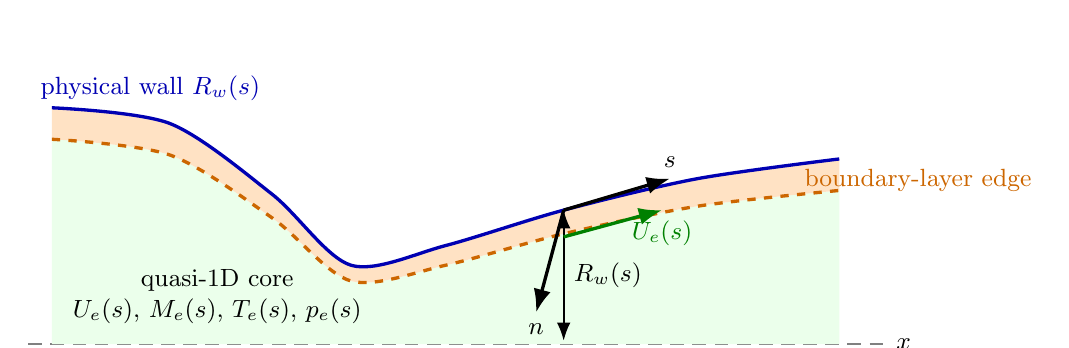
\begin{tikzpicture}[
    scale=1.0,
    >=Latex,
    every node/.style={font=\small}
]

% Centreline
\draw[dash pattern=on 5pt off 3pt,gray]
    (-0.3,0) -- (10.6,0)
    node[right,black] {\(x\)};

% Inviscid core
\fill[green!8]
    (0,0)
    -- plot[smooth] coordinates {
        (0,2.60)
        (1.5,2.40)
        (2.8,1.60)
        (3.8,0.80)
        (5.0,1.00)
        (6.5,1.40)
        (8.2,1.75)
        (10.0,1.95)
    }
    -- (10.0,0)
    -- cycle;

% Boundary-layer region
\fill[orange!23]
    plot[smooth] coordinates {
        (0,3.00)
        (1.5,2.80)
        (2.8,1.90)
        (3.8,1.00)
        (5.0,1.25)
        (6.5,1.70)
        (8.2,2.10)
        (10.0,2.35)
    }
    --
    plot[smooth] coordinates {
        (10.0,1.95)
        (8.2,1.75)
        (6.5,1.40)
        (5.0,1.00)
        (3.8,0.80)
        (2.8,1.60)
        (1.5,2.40)
        (0,2.60)
    }
    -- cycle;

% Physical wall
\draw[very thick,blue!70!black]
    plot[smooth] coordinates {
        (0,3.00)
        (1.5,2.80)
        (2.8,1.90)
        (3.8,1.00)
        (5.0,1.25)
        (6.5,1.70)
        (8.2,2.10)
        (10.0,2.35)
    };

% BL edge
\draw[very thick,dashed,orange!80!black]
    plot[smooth] coordinates {
        (0,2.60)
        (1.5,2.40)
        (2.8,1.60)
        (3.8,0.80)
        (5.0,1.00)
        (6.5,1.40)
        (8.2,1.75)
        (10.0,1.95)
    };

\node[blue!70!black] at (1.25,3.25)
    {physical wall \(R_w(s)\)};

\node[orange!80!black] at (11,2.08)
    {boundary-layer edge};

\node[align=center] at (2.1,0.6)
    {quasi-1D core\\
    \(U_e(s),\,M_e(s),\,T_e(s),\,p_e(s)\)};

% Selected wall point
\coordinate (W) at (6.5,1.70);
\coordinate (E) at (6.5,1.40);

% Local tangent
\draw[->,very thick] (W) -- ++(1.35,0.4)
    node[above] {\(s\)};

% Local normal
\draw[->,very thick] (W) -- ++(-0.35,-1.30)
    node[below] {\(n\)};

% Local radius
\draw[<->,thick]
    (6.5,0.04) -- (6.5,1.70)
    node[midway,right] {\(R_w(s)\)};

% Edge velocity
\draw[->,very thick,green!50!black]
    (6.5,1.36) -- ++(1.25,0.34)
    node[below] {\(U_e(s)\)};

\end{tikzpicture}
\caption{Quasi-one-dimensional core and wall-fitted coordinates used by the
integral boundary-layer model.}
\label{fig:core_BL_coordinates}
\end{figure}

No additional resolved spatial dimension is introduced by the mapping
\(x\leftrightarrow s\). The inviscid core remains quasi-one-dimensional, and
the transported integral boundary-layer variables are also functions of the
single coordinate \(s\).

% ---------------------------------------------------------
\subsection{Velocity Components Inside the Boundary Layer}
% ---------------------------------------------------------

The actual local velocity field inside the boundary layer contains tangential
and wall-normal components:

\begin{equation}
    \boxed{
    \boldsymbol{u}(s,n)
    =
    u_s(s,n)\boldsymbol{e}_s
    +
    u_n(s,n)\boldsymbol{e}_n
    }.
    \label{eq:BL_velocity_decomposition}
\end{equation}

Here,

\begin{itemize}
    \item \(u_s(s,n)\) is the velocity component tangent to the wall;
    \item \(u_n(s,n)\) is the velocity component normal to the wall;
    \item \(U_e(s)\) is the one-dimensional tangential velocity at the
    boundary-layer edge.
\end{itemize}

At a stationary, impermeable, no-slip wall,

\begin{equation}
    \boxed{
    u_s(s,0)=0,
    \qquad
    u_n(s,0)=0
    }.
    \label{eq:BL_wall_conditions}
\end{equation}

At the outer edge of the boundary layer,

\begin{equation}
    u_s\bigl(s,\delta(s)\bigr)\simeq U_e(s),
    \qquad
    \tau_{sn}\bigl(s,\delta(s)\bigr)\simeq0.
    \label{eq:BL_edge_conditions}
\end{equation}

The wall-normal component is zero at the impermeable wall but is generally
nonzero inside the boundary layer:

\begin{equation}
    u_n(s,n)\neq0,
    \qquad
    0<n\leq\delta(s).
    \label{eq:normal_velocity_nonzero}
\end{equation}

Its magnitude is normally much smaller than the tangential velocity:

\begin{equation}
    |u_n|\ll|u_s|.
    \label{eq:BL_velocity_scaling}
\end{equation}

Nevertheless, the normal convection term cannot be discarded because the
normal velocity gradient is large inside a thin boundary layer. In general,

\begin{equation}
    u_n\frac{\partial u_s}{\partial n}
\end{equation}

can be of the same asymptotic order as

\begin{equation}
    u_s\frac{\partial u_s}{\partial s}.
\end{equation}

The present model does not explicitly resolve
\(u_s(s,n)\), \(u_n(s,n)\), \(T(s,n)\), or \(\rho(s,n)\). These
two-dimensional fields appear in the theoretical definitions and derivation,
but their integrated effects are represented by one-dimensional
boundary-layer variables.

% ---------------------------------------------------------
\subsection{Physical and Integral Boundary-Layer Thicknesses}
% ---------------------------------------------------------

Three different boundary-layer thicknesses are employed:

\begin{equation}
    \boxed{
    \delta(s),\qquad
    \delta^*(s),\qquad
    \theta(s)
    }.
\end{equation}

Although all three quantities have dimensions of length, they represent
different physical effects.

\begin{figure}[htbp]
\centering
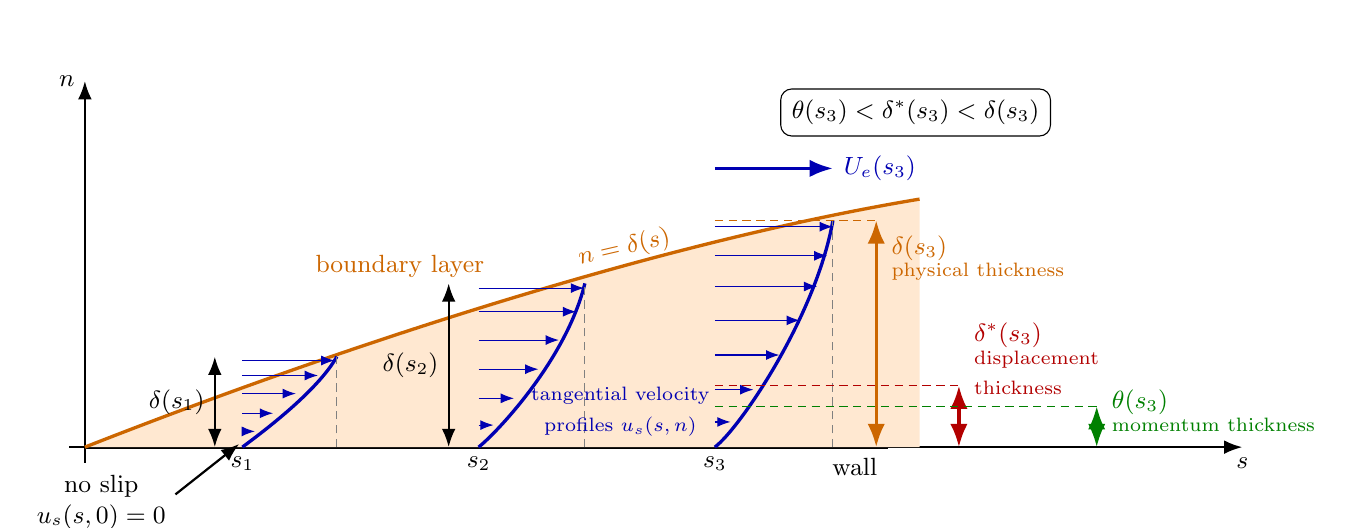
\begin{tikzpicture}[
    x=1.0cm,
    y=1.0cm,
    >=Latex,
    every node/.style={font=\small}
]

% ---------------------------------------------------------
% Coordinates
% ---------------------------------------------------------

\draw[->,thick] (-0.2,0) -- (14.7,0)
    node[below] {\(s\)};

\draw[->,thick] (0,-0.2) -- (0,4.65)
    node[left] {\(n\)};

% Wall
\draw[very thick] (0,0) -- (10.2,0)
    node[below left] {wall};

% ---------------------------------------------------------
% Boundary-layer region
% ---------------------------------------------------------

\fill[orange!18]
    (0,0)
    .. controls (2.8,1.10) and (7.0,2.55) ..
    (10.6,3.15)
    -- (10.6,0)
    -- cycle;

\draw[very thick,orange!80!black]
    (0,0)
    .. controls (2.8,1.10) and (7.0,2.55) ..
    (10.6,3.15);

\node[orange!80!black,rotate=13]
    at (6.85,2.53)
    {\(n=\delta(s)\)};

\node[orange!80!black]
    at (4.0,2.30)
    {boundary layer};

% ---------------------------------------------------------
% Velocity profile at s_1
% ---------------------------------------------------------

\draw[very thick,blue!70!black]
    (2.0,0)
    .. controls (2.20,0.15) and (2.95,0.70) ..
    (3.20,1.15);

\foreach \yy/\xx in {
    0.20/2.16,
    0.43/2.39,
    0.68/2.68,
    0.91/2.96,
    1.10/3.17
}{
    \draw[->,blue!70!black]
        (2.0,\yy) -- (\xx,\yy);
}

\draw[densely dashed,gray]
    (3.20,0) -- (3.20,1.15);

\draw[<->,thick]
    (1.65,0) -- (1.65,1.15)
    node[midway,left] {\(\delta(s_1)\)};

\node[below] at (2.0,0) {\(s_1\)};

% ---------------------------------------------------------
% Velocity profile at s_2
% ---------------------------------------------------------

\draw[very thick,blue!70!black]
    (5.0,0)
    .. controls (5.25,0.20) and (6.12,1.13) ..
    (6.35,2.08);

\foreach \yy/\xx in {
    0.28/5.19,
    0.62/5.45,
    0.99/5.76,
    1.36/6.02,
    1.72/6.24,
    2.02/6.34
}{
    \draw[->,blue!70!black]
        (5.0,\yy) -- (\xx,\yy);
}

\draw[densely dashed,gray]
    (6.35,0) -- (6.35,2.08);

\draw[<->,thick]
    (4.62,0) -- (4.62,2.08)
    node[midway,left] {\(\delta(s_2)\)};

\node[below] at (5.0,0) {\(s_2\)};

% ---------------------------------------------------------
% Velocity profile at s_3
% ---------------------------------------------------------

\draw[very thick,blue!70!black]
    (8.0,0)
    .. controls (8.30,0.22) and (9.28,1.64) ..
    (9.50,2.88);

\foreach \yy/\xx in {
    0.32/8.20,
    0.73/8.49,
    1.17/8.82,
    1.61/9.08,
    2.04/9.30,
    2.43/9.43,
    2.80/9.50
}{
    \draw[->,blue!70!black]
        (8.0,\yy) -- (\xx,\yy);
}

\draw[densely dashed,gray]
    (9.50,0) -- (9.50,2.88);

\node[below] at (8.0,0) {\(s_3\)};

% Edge velocity
\draw[->,very thick,blue!70!black]
    (8.0,3.54) -- (9.50,3.54)
    node[right] {\(U_e(s_3)\)};

% ---------------------------------------------------------
% Physical and equivalent thicknesses at s_3
% Values are schematic, not quantitatively scaled
% ---------------------------------------------------------

% Momentum thickness theta
% Displacement thickness delta*  (fica primeiro / mais à esquerda)
\draw[densely dashed,red!70!black]
    (8.0,0.78) -- (11.10,0.78);

\draw[<->,very thick,red!70!black]
    (11.10,0) -- (11.10,0.78);

\node[
    right,
    red!70!black,
    align=left
] at (11.17,1.12)
    {\(\delta^*(s_3)\)\\[-1mm]
     \scriptsize displacement\\ \scriptsize thickness};


% Momentum thickness theta  (fica depois / mais à direita)
\draw[densely dashed,green!50!black]
    (8.0,0.52) -- (12.85,0.52);

\draw[<->,very thick,green!50!black]
    (12.85,0) -- (12.85,0.52);

\node[
    right,
    green!50!black,
    align=left
] at (12.92,0.46)
    {\(\theta(s_3)\)\\[-1mm]
     \scriptsize momentum thickness};

% Physical thickness delta
\draw[densely dashed,orange!80!black]
    (8.0,2.88) -- (10.05,2.88);

\draw[<->,very thick,orange!80!black]
    (10.05,0) -- (10.05,2.88);

\node[
    right,
    orange!80!black,
    align=left
] at (10.12,2.40)
    {\(\delta(s_3)\)\\[-1mm]
     \scriptsize physical thickness};

% Ordering
\node[
    draw,
    rounded corners,
    fill=white,
    align=center,
    inner sep=4pt
] at (10.55,4.25)
    {\(\theta(s_3)<\delta^*(s_3)<\delta(s_3)\)};

% Clarification

% ---------------------------------------------------------
% No-slip condition
% ---------------------------------------------------------

\draw[->,thick]
    (1.15,-0.60) -- (1.96,0.04);

\node[align=center,left]
    at (1.15,-0.70)
    {no slip\\\(u_s(s,0)=0\)};

% Profile label
\node[
    blue!70!black,
    align=center
] at (6.8,0.45)
    {\scriptsize tangential velocity\\ \scriptsize profiles \(u_s(s,n)\)};

\end{tikzpicture}

\caption{Development of the tangential velocity profile along the nozzle
wall and comparison of the conventional boundary-layer thickness
\(\delta\), displacement thickness \(\delta^*\), and momentum thickness
\(\theta\) at station \(s_3\). The coordinate \(n\) is normal to the wall,
whereas \(s\) follows the wall in the streamwise direction. The displayed
relative magnitudes of \(\theta\) and \(\delta^*\) are schematic and are not
drawn to scale.}

\label{fig:BL_velocity_growth}
\end{figure}
\subsubsection{Representative physical thickness}

The velocity approaches \(U_e\) asymptotically, and therefore the boundary
layer does not possess an exact physical edge. A common engineering convention
is to identify its thickness with the wall-normal location at which

\begin{equation}
    \frac{u_s}{U_e}\simeq0.99.
    \label{eq:delta_99_definition}
\end{equation}

The quantity \(\delta(s)\) is consequently interpreted as a representative
physical thickness of the velocity-gradient region. In the profile closure
introduced below, it is treated as the outer scale of the assumed velocity
profile and is approximately identified with the conventional
\(\delta_{99}\).

\subsubsection{Compressible displacement thickness}

Inside the boundary layer, the local mass flux \(\rho u_s\) is smaller than
the mass flux \(\rho_eU_e\) that would exist if the inviscid edge state
extended uniformly to the physical wall.

The mass-flow deficit per unit wetted perimeter is

\begin{equation}
    \dot{m}'_{\mathrm{def}}(s)
    =
    \int_0^{\delta(s)}
    \left[
        \rho_e(s)U_e(s)
        -
        \rho(s,n)u_s(s,n)
    \right]dn.
    \label{eq:mass_flow_deficit}
\end{equation}

Factoring out the edge mass flux gives

\begin{equation}
    \dot{m}'_{\mathrm{def}}(s)
    =
    \rho_e(s)U_e(s)
    \int_0^{\delta(s)}
    \left[
        1-
        \frac{
            \rho(s,n)u_s(s,n)
        }{
            \rho_e(s)U_e(s)
        }
    \right]dn.
\end{equation}

The compressible displacement thickness is therefore defined as

\begin{equation}
    \boxed{
    \delta^*(s)
    =
    \int_0^{\delta(s)}
    \left[
        1-
        \frac{
            \rho(s,n)u_s(s,n)
        }{
            \rho_e(s)U_e(s)
        }
    \right]dn
    }.
    \label{eq:compressible_displacement_thickness}
\end{equation}

It follows that

\begin{equation}
    \boxed{
    \dot{m}'_{\mathrm{def}}(s)
    =
    \rho_e(s)U_e(s)\delta^*(s)
    }.
    \label{eq:mass_deficit_displacement}
\end{equation}

The displacement thickness is the thickness of a hypothetical region carrying
zero mass flow that would produce the same mass-flow deficit as the actual
boundary layer.

Equivalently, the inviscid core behaves approximately as if the solid wall
were displaced towards the nozzle axis by \(\delta^*\). Under the thin-layer
approximation, the effective core radius is

\begin{equation}
    \boxed{
    R_{\mathrm{eff}}(s)
    =
    R_w(s)-\delta^*(s)
    }.
    \label{eq:effective_radius_displacement}
\end{equation}

The displacement thickness is not the physical location of the
boundary-layer edge. Generally,

\begin{equation}
    \delta^*(s)<\delta(s).
    \label{eq:displacement_less_than_delta}
\end{equation}

\subsubsection{Compressible momentum thickness}

The reduced tangential velocity also produces a deficit in streamwise
momentum flux. The momentum-flux deficit per unit wetted perimeter is

\begin{equation}
    D_m'(s)
    =
    \int_0^{\delta(s)}
    \rho(s,n)u_s(s,n)
    \left[
        U_e(s)-u_s(s,n)
    \right]dn.
    \label{eq:momentum_deficit_integral}
\end{equation}

Introducing the edge quantities gives

\begin{equation}
\begin{split}
    D_m'(s)
    &=
    \rho_e(s)U_e^2(s)
    \int_0^{\delta(s)}
    \frac{
        \rho(s,n)u_s(s,n)
    }{
        \rho_e(s)U_e(s)
    }
    \left[
        1-
        \frac{
            u_s(s,n)
        }{
            U_e(s)
        }
    \right]dn.
\end{split}
\label{eq:momentum_deficit_normalized}
\end{equation}

The compressible momentum thickness is defined as

\begin{equation}
    \boxed{
    \theta(s)
    =
    \int_0^{\delta(s)}
    \frac{
        \rho(s,n)u_s(s,n)
    }{
        \rho_e(s)U_e(s)
    }
    \left[
        1-
        \frac{
            u_s(s,n)
        }{
            U_e(s)
        }
    \right]dn
    }.
    \label{eq:compressible_momentum_thickness}
\end{equation}

Consequently,

\begin{equation}
    \boxed{
    D_m'(s)
    =
    \rho_e(s)U_e^2(s)\theta(s)
    },
    \qquad
    [D_m']=\mathrm{N\,m^{-1}}.
    \label{eq:momentum_deficit_per_perimeter}
\end{equation}

The momentum thickness is the thickness of a hypothetical region producing
the same momentum-flux deficit as the actual velocity and density profiles. It
is not itself momentum and does not represent a physical interface inside the
boundary layer.

For the complete circumference of an axisymmetric nozzle,

\begin{equation}
    \boxed{
    D_m(s)
    =
    P_w(s)\rho_e(s)U_e^2(s)\theta(s)
    }
    \label{eq:axisymmetric_momentum_deficit}
\end{equation}

or, using \(P_w=2\pi R_w\),

\begin{equation}
    \boxed{
    D_m(s)
    =
    2\pi R_w(s)\rho_e(s)U_e^2(s)\theta(s)
    },
    \qquad
    [D_m]=\mathrm{N}.
    \label{eq:axisymmetric_momentum_deficit_radius}
\end{equation}

The three thicknesses can therefore be summarized as

\begin{align}
    \delta
    &:
    &&\text{representative physical extent of the velocity-gradient region},
    \\
    \delta^*
    &:
    &&\text{equivalent thickness associated with mass-flow deficit},
    \\
    \theta
    &:
    &&\text{equivalent thickness associated with momentum-flux deficit}.
\end{align}

For a conventional attached turbulent boundary layer, the typical ordering is

\begin{equation}
    \boxed{
    \theta(s)<\delta^*(s)<\delta(s)
    }.
    \label{eq:BL_thickness_ordering}
\end{equation}

The ratio

\begin{equation}
    \boxed{
    H(s)
    =
    \frac{\delta^*(s)}{\theta(s)}
    }
    \label{eq:shape_factor}
\end{equation}

is the compressible boundary-layer shape factor. It provides an integral
measure of the shapes of the velocity and density profiles.

Figure~\ref{fig:BL_thicknesses} illustrates the different meanings of
\(\delta\), \(\delta^*\), and \(\theta\).

\begin{figure}[htbp]
\centering
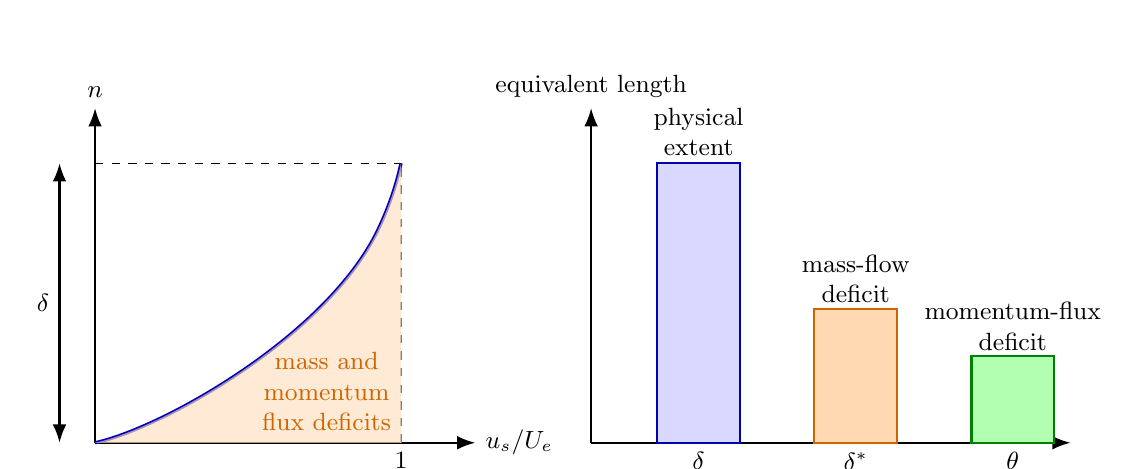
\begin{tikzpicture}[
    x=1.05cm,
    y=1.0cm,
    >=Latex,
    every node/.style={font=\small}
]

% Axes
\draw[->,thick] (0,0) -- (4.6,0)
    node[right] {\(u_s/U_e\)};
\draw[->,thick] (0,0) -- (0,4.25)
    node[above] {\(n\)};

% Edge velocity
\draw[dashed,gray]
    (3.7,0) -- (3.7,3.55);
\node[below] at (3.7,0) {\(1\)};

% Velocity profile
\draw[very thick,blue!70!black]
    (0,0)
    .. controls (0.8,0.18) and (2.8,1.35) ..
    (3.42,2.70)
    .. controls (3.58,3.05) and (3.66,3.35) ..
    (3.70,3.55);

% Deficit area
\fill[orange!25,opacity=0.65]
    (3.7,0)
    -- (0,0)
    .. controls (0.8,0.18) and (2.8,1.35) ..
    (3.42,2.70)
    .. controls (3.58,3.05) and (3.66,3.35) ..
    (3.70,3.55)
    -- cycle;

% Delta
\draw[<->,thick]
    (-0.43,0) -- (-0.43,3.55)
    node[midway,left] {\(\delta\)};
\draw[dashed] (0,3.55) -- (3.70,3.55);

\node[align=center,orange!80!black]
    at (2.8,0.65)
    {mass and\\ momentum\\flux deficits};

% Equivalent bars
\draw[->,thick] (6.0,0) -- (11.8,0);
\draw[->,thick] (6.0,0) -- (6.0,4.25)
    node[above] {equivalent length};

\fill[blue!15] (6.8,0) rectangle (7.8,3.55);
\draw[thick,blue!70!black] (6.8,0) rectangle (7.8,3.55);
\node[below] at (7.3,0) {\(\delta\)};
\node[align=center] at (7.3,3.95) {physical\\extent};

\fill[orange!30] (8.7,0) rectangle (9.7,1.70);
\draw[thick,orange!80!black] (8.7,0) rectangle (9.7,1.70);
\node[below] at (9.2,0) {\(\delta^*\)};
\node[align=center] at (9.2,2.08) {mass-flow\\deficit};

\fill[green!30] (10.6,0) rectangle (11.6,1.10);
\draw[thick,green!50!black] (10.6,0) rectangle (11.6,1.10);
\node[below] at (11.1,0) {\(\theta\)};
\node[align=center] at (11.1,1.48) {momentum-flux\\deficit};

\end{tikzpicture}

\caption{Physical interpretation of the representative boundary-layer
thickness \(\delta\), displacement thickness \(\delta^*\), and momentum
thickness \(\theta\). The relative dimensions are schematic and not to
scale.}
\label{fig:BL_thicknesses}
\end{figure}

% ---------------------------------------------------------
\subsection{Normalized Profile Closure}
% ---------------------------------------------------------

The definitions of \(\delta^*\) and \(\theta\) depend on the wall-normal
profiles

\begin{equation}
    u_s(s,n),\qquad
    T(s,n),\qquad
    \rho(s,n),
\end{equation}

and on the physical thickness \(\delta(s)\). These quantities are not provided
by the quasi-one-dimensional core model.

To evaluate the shape factor without resolving the complete two-dimensional
boundary layer, normalized velocity, temperature, and density profiles are
introduced.

\subsubsection{Normalized wall-normal coordinate}

The dimensionless coordinate

\begin{equation}
    \boxed{
    \eta
    =
    \frac{n}{\delta(s)}
    },
    \qquad
    0\leq\eta\leq1,
    \label{eq:normalized_wall_coordinate}
\end{equation}

maps the boundary layer at every streamwise station onto the same normalized
interval.

Thus,

\begin{align}
    \eta=0
    &\quad\Longleftrightarrow\quad
    n=0,
    &&\text{wall},
    \\
    \eta=1
    &\quad\Longleftrightarrow\quad
    n=\delta(s),
    &&\text{representative boundary-layer edge}.
\end{align}

The dimensional and normalized coordinates are related by

\begin{equation}
    n=\eta\delta(s),
    \qquad
    dn=\delta(s)\,d\eta.
    \label{eq:normal_coordinate_transformation}
\end{equation}

The coordinate \(\eta\) is not an additional resolved spatial dimension. It is
an auxiliary quadrature coordinate used to describe the assumed shapes of the
unresolved profiles.

The normalization is useful because \(\delta(s)\) is not initially known.
Although the dimensional values of \(\delta^*\) and \(\theta\) cannot yet be
calculated from their definitions, their ratios to \(\delta\) can be
calculated using normalized profiles.

\subsubsection{One-seventh-power velocity profile}

The tangential velocity profile is approximated using the empirical turbulent
one-seventh-power law:

\begin{equation}
    \boxed{
    f(\eta)
    \equiv
    \frac{u_s(s,n)}{U_e(s)}
    =
    \eta^{1/7}
    }.
    \label{eq:one_seventh_velocity_profile}
\end{equation}

The profile satisfies the idealized boundary conditions

\begin{equation}
    f(0)=0,
    \qquad
    f(1)=1.
\end{equation}

The first condition represents no slip at the wall. The second condition
matches the assumed profile to the edge velocity. The conventional
\(99\%\) definition of \(\delta\) and the condition \(f(1)=1\) are treated as
equivalent engineering representations of the boundary-layer edge.

The one-seventh-power law prescribes only the normalized shape of the velocity
profile. It does not determine the dimensional thickness \(\delta(s)\).

Figure~\ref{fig:normalized_BL_profiles} illustrates the normalized coordinate
and the assumed velocity and temperature profiles.

\begin{figure}[htbp]
\centering
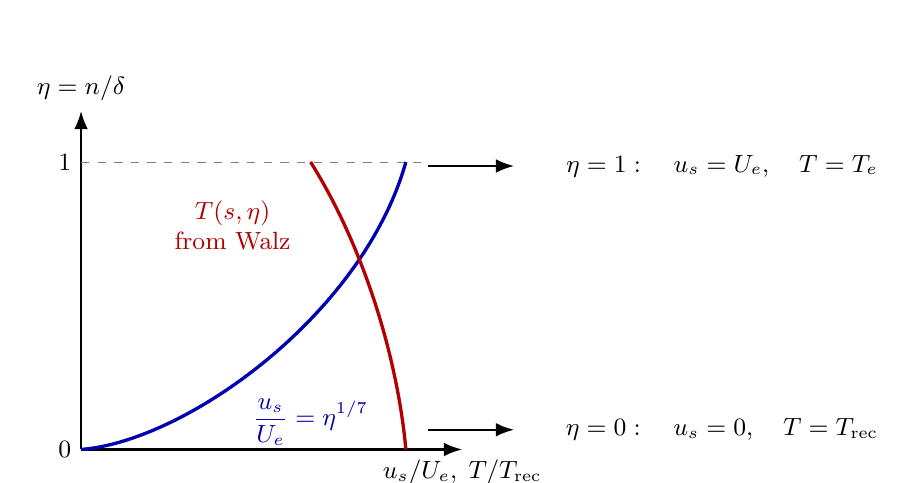
\begin{tikzpicture}[
    x=1.1cm,
    y=1.0cm,
    >=Latex,
    every node/.style={font=\small}
]

% Coordinate axes
\draw[->,thick] (0,0) -- (4.4,0)
    node[below] {\(u_s/U_e,\;T/T_{\mathrm{rec}}\)};
\draw[->,thick] (0,0) -- (0,4.3)
    node[above] {\(\eta=n/\delta\)};

% Eta boundaries
\draw[dashed,gray] (0,3.65) -- (4.0,3.65);
\node[left] at (0,3.65) {\(1\)};
\node[left] at (0,0) {\(0\)};

% Velocity profile
\draw[very thick,blue!70!black]
    (0,0)
    .. controls (1.20,0.10) and (3.25,1.70) ..
    (3.75,3.65);

\node[blue!70!black,align=center]
    at (2.65,0.35)
    {\(\displaystyle
      \frac{u_s}{U_e}=\eta^{1/7}\)};

% Temperature profile
\draw[very thick,red!70!black]
    (3.75,0)
    .. controls (3.65,1.20) and (3.25,2.60) ..
    (2.65,3.65);

\node[red!70!black,align=center]
    at (1.75,2.85)
    {\(T(s,\eta)\)\\from Walz};

% Wall and edge
\node[align=left] at (7.4,0.25)
    {\(\eta=0:\quad u_s=0,\quad T=T_{\mathrm{rec}}\)};

\node[align=left] at (7.4,3.60)
    {\(\eta=1:\quad u_s=U_e,\quad T=T_e\)};

\draw[->,thick] (4.0,0.25) -- (5.0,0.25);
\draw[->,thick] (4.0,3.60) -- (5.0,3.60);

\end{tikzpicture}

\caption{Normalized wall-normal coordinate and assumed profiles for an
adiabatic compressible turbulent boundary layer. The diagram is schematic.}
\label{fig:normalized_BL_profiles}
\end{figure}

\subsubsection{Recovery temperature and adiabatic wall}

The static edge temperature \(T_e(s)\) does not represent the complete
temperature distribution across the boundary layer. In compressible flow,
part of the kinetic energy is recovered as internal energy near the wall.

The corresponding recovery temperature is

\begin{equation}
    \boxed{
    T_{\mathrm{rec}}(s)
    =
    T_e(s)
    \left[
        1+
        r_{\mathrm{rec}}(s)
        \frac{\gamma_e(s)-1}{2}
        M_e^2(s)
    \right]
    },
    \label{eq:recovery_temperature}
\end{equation}

where \(r_{\mathrm{rec}}\) is the recovery factor. For a turbulent boundary
layer,

\begin{equation}
    \boxed{
    r_{\mathrm{rec}}(s)
    \simeq
    Pr_e^{1/3}(s)
    }.
    \label{eq:turbulent_recovery_factor}
\end{equation}

The recovery temperature is the temperature approached by an adiabatic wall
under the local edge-flow conditions. It is generally bounded by

\begin{equation}
    T_e(s)
    \leq
    T_{\mathrm{rec}}(s)
    \leq
    T_0(s),
\end{equation}

where \(T_0\) is the local stagnation temperature.

The present model assumes an adiabatic wall:

\begin{equation}
    q_w''=0.
\end{equation}

Consequently,

\begin{equation}
    \boxed{
    T_w(s)=T_{\mathrm{rec}}(s)
    }.
    \label{eq:quick_adiabatic_wall_temperature}
\end{equation}

The wall temperature is therefore not an independent prescribed input in the
adiabatic boundary-layer closure.

\subsubsection{Walz temperature--velocity relation}

The density profile required by \(\delta^*\) and \(\theta\) depends on the
temperature across the boundary layer. Since the present model does not solve
a wall-normal energy equation, the temperature profile is approximated using
the Walz temperature--velocity relation.

For a general wall temperature, the Walz relation is

\begin{equation}
    \boxed{
    T(s,\eta)
    =
    T_w(s)
    +
    \left[
        T_{\mathrm{rec}}(s)-T_w(s)
    \right]f(\eta)
    -
    \left[
        T_{\mathrm{rec}}(s)-T_e(s)
    \right]f^2(\eta)
    }.
    \label{eq:general_walz_relation}
\end{equation}

There is no single quantity referred to here as the ``Walz temperature.''
Equation~\eqref{eq:general_walz_relation} provides the complete approximate
temperature profile

\begin{equation}
    T=T(s,\eta)
\end{equation}

as a function of the local normalized velocity \(f=u_s/U_e\).

Under the adiabatic-wall condition \(T_w=T_{\mathrm{rec}}\), the linear term
vanishes and the relation reduces to

\begin{equation}
    \boxed{
    T(s,\eta)
    =
    T_{\mathrm{rec}}(s)
    -
    \left[
        T_{\mathrm{rec}}(s)-T_e(s)
    \right]f^2(\eta)
    }.
    \label{eq:adiabatic_walz_relation}
\end{equation}

Using \(f(\eta)=\eta^{1/7}\),

\begin{equation}
    \boxed{
    T(s,\eta)
    =
    T_{\mathrm{rec}}(s)
    -
    \left[
        T_{\mathrm{rec}}(s)-T_e(s)
    \right]\eta^{2/7}
    }.
    \label{eq:adiabatic_walz_eta}
\end{equation}

The limiting values are

\begin{align}
    T(s,0)
    &=
    T_{\mathrm{rec}}(s)
    =
    T_w(s),
    \\
    T(s,1)
    &=
    T_e(s).
\end{align}

The relation therefore describes the temperature variation from the recovery
temperature at the adiabatic wall to the static edge temperature at the outer
boundary of the layer.

\subsubsection{Normalized density profile}

The thin-boundary-layer approximation implies that the static pressure is
approximately uniform in the wall-normal direction:

\begin{equation}
    \boxed{
    p(s,n)\simeq p_e(s)
    },
    \qquad
    \frac{\partial p}{\partial n}\simeq0.
    \label{eq:normal_pressure_uniformity}
\end{equation}

This does not imply that the density is uniform across the boundary layer.
Since

\begin{equation}
    T=T(s,n),
\end{equation}

the density also depends on the wall-normal coordinate:

\begin{equation}
    \rho=\rho(s,n).
\end{equation}

Assuming ideal-gas behavior and an approximately uniform specific gas
constant across the thin layer,

\begin{align}
    \rho(s,\eta)
    &=
    \frac{p_e(s)}
         {R_g(s)T(s,\eta)},
    \\
    \rho_e(s)
    &=
    \frac{p_e(s)}
         {R_g(s)T_e(s)}.
\end{align}

Dividing these expressions gives the normalized density profile

\begin{equation}
    \boxed{
    \frac{\rho(s,\eta)}{\rho_e(s)}
    =
    \frac{T_e(s)}{T(s,\eta)}
    }.
    \label{eq:normalized_density_profile}
\end{equation}

The assumed profile closure can therefore be summarized as

\begin{equation}
    \boxed{
    \eta
    \longrightarrow
    \frac{u_s}{U_e}
    \longrightarrow
    T(s,\eta)
    \longrightarrow
    \frac{\rho(s,\eta)}{\rho_e(s)}
    }.
    \label{eq:profile_closure_sequence}
\end{equation}

The one-seventh-power law provides the normalized velocity profile, the Walz
relation provides the corresponding temperature profile, and the ideal-gas
relation provides the density profile required by the compressible integral
thicknesses.

\subsubsection{Normalized integral thicknesses}

Using

\begin{equation}
    n=\eta\delta(s),
    \qquad
    dn=\delta(s)\,d\eta,
\end{equation}

the displacement thickness becomes

\begin{equation}
\begin{split}
    \delta^*(s)
    &=
    \delta(s)
    \int_0^1
    \left[
        1-
        \frac{\rho(s,\eta)}{\rho_e(s)}
        f(\eta)
    \right]d\eta.
\end{split}
\label{eq:normalized_displacement_thickness}
\end{equation}

The dimensionless displacement-thickness ratio is therefore

\begin{equation}
    \boxed{
    I_{\delta^*}(s)
    \equiv
    \frac{\delta^*(s)}{\delta(s)}
    =
    \int_0^1
    \left[
        1-
        \frac{\rho(s,\eta)}{\rho_e(s)}
        f(\eta)
    \right]d\eta
    }.
    \label{eq:displacement_thickness_ratio}
\end{equation}

Similarly, the momentum thickness becomes

\begin{equation}
\begin{split}
    \theta(s)
    &=
    \delta(s)
    \int_0^1
    \frac{\rho(s,\eta)}{\rho_e(s)}
    f(\eta)
    \left[
        1-f(\eta)
    \right]d\eta.
\end{split}
\label{eq:normalized_momentum_thickness}
\end{equation}

The corresponding dimensionless ratio is

\begin{equation}
    \boxed{
    I_\theta(s)
    \equiv
    \frac{\theta(s)}{\delta(s)}
    =
    \int_0^1
    \frac{\rho(s,\eta)}{\rho_e(s)}
    f(\eta)
    \left[
        1-f(\eta)
    \right]d\eta
    }.
    \label{eq:momentum_thickness_ratio}
\end{equation}

At this stage, the dimensional boundary-layer thickness \(\delta(s)\) remains
unknown. Consequently, these profile integrations do not directly provide
\(\delta^*\) or \(\theta\) in metres.

However, the unknown thickness cancels in their ratio:

\begin{equation}
\begin{split}
    H(s)
    &=
    \frac{\delta^*(s)}{\theta(s)}
    =
    \frac{
        \delta(s)I_{\delta^*}(s)
    }{
        \delta(s)I_\theta(s)
    }.
\end{split}
\end{equation}

Therefore,

\begin{equation}
    \boxed{
    H(s)
    =
    \frac{I_{\delta^*}(s)}
         {I_\theta(s)}
    }
    \label{eq:shape_factor_ratio}
\end{equation}

or, explicitly,

\begin{equation}
    \boxed{
    H(s)
    =
    \frac{
        \displaystyle
        \int_0^1
        \left[
            1-
            \frac{\rho}{\rho_e}f
        \right]d\eta
    }{
        \displaystyle
        \int_0^1
        \frac{\rho}{\rho_e}
        f(1-f)\,d\eta
    }
    }.
    \label{eq:shape_factor_profile_closure}
\end{equation}

This cancellation is the principal reason for introducing the normalized
coordinate \(\eta\). The shape factor can be calculated before the dimensional
boundary-layer thickness is known.

Numerically, the interval \(0\leq\eta\leq1\) is divided into a set of
quadrature points. At every streamwise station \(s_i\), the model evaluates

\begin{equation}
    f(\eta_j),\qquad
    T(s_i,\eta_j),\qquad
    \frac{\rho(s_i,\eta_j)}{\rho_e(s_i)},
\end{equation}

and integrates Eqs.~\eqref{eq:displacement_thickness_ratio} and
\eqref{eq:momentum_thickness_ratio} using the trapezoidal rule.

Once \(\theta(s)\) has been obtained from the integral momentum equation, the
remaining thicknesses can be recovered from

\begin{equation}
    \boxed{
    \delta^*(s)=H(s)\theta(s)
    }
    \label{eq:delta_star_from_H_theta}
\end{equation}

and

\begin{equation}
    \boxed{
    \delta(s)
    =
    \frac{\theta(s)}
         {I_\theta(s)}
    }.
    \label{eq:physical_delta_from_theta}
\end{equation}

% ---------------------------------------------------------
\subsection{Local Conservative Momentum Equation}
% ---------------------------------------------------------

For statistically steady flow,

\begin{equation}
    \frac{\partial(\rho\boldsymbol{u})}{\partial t}=0.
    \label{eq:steady_momentum_condition}
\end{equation}

The conservative momentum equation therefore reduces to

\begin{equation}
    \nabla\cdot
    \left(
        \rho\boldsymbol{u}\otimes\boldsymbol{u}
    \right)
    =
    -\nabla p
    +
    \nabla\cdot\boldsymbol{\tau}.
    \label{eq:steady_conservative_momentum}
\end{equation}

Resolving this equation in the direction tangent to the wall gives

\begin{equation}
    \frac{\partial(\rho u_s^2)}{\partial s}
    +
    \frac{\partial(\rho u_nu_s)}{\partial n}
    =
    -\frac{\partial p}{\partial s}
    +
    \frac{\partial\tau_{ss}}{\partial s}
    +
    \frac{\partial\tau_{sn}}{\partial n}.
    \label{eq:local_tangential_momentum}
\end{equation}

The first two terms represent the tangential and normal convective transport
of tangential momentum. The last two terms represent the tangential and normal
diffusive transport of tangential momentum.

For a thin boundary layer,

\begin{equation}
    \delta\ll L,
    \qquad
    \frac{\partial}{\partial n}
    \gg
    \frac{\partial}{\partial s}.
    \label{eq:thin_BL_scale}
\end{equation}

Consequently, the streamwise diffusion of tangential momentum is much smaller
than its wall-normal diffusion:

\begin{equation}
    \frac{\partial\tau_{ss}}{\partial s}
    \ll
    \frac{\partial\tau_{sn}}{\partial n}.
    \label{eq:negligible_streamwise_diffusion}
\end{equation}

Using also \(p(s,n)\simeq p_e(s)\), the local tangential momentum equation
reduces to

\begin{equation}
    \boxed{
    \frac{\partial(\rho u_s^2)}{\partial s}
    +
    \frac{\partial(\rho u_nu_s)}{\partial n}
    =
    -\frac{dp_e}{ds}
    +
    \frac{\partial\tau_{sn}}{\partial n}
    }.
    \label{eq:reduced_tangential_momentum}
\end{equation}

The corresponding steady continuity equation is

\begin{equation}
    \nabla\cdot(\rho\boldsymbol{u})=0.
    \label{eq:steady_continuity_BL}
\end{equation}

For a thin axisymmetric boundary layer, it can be expressed approximately in
perimeter-weighted form as

\begin{equation}
    \boxed{
    \frac{\partial}{\partial s}
    \left[
        P_w(s)\rho u_s
    \right]
    +
    \frac{\partial}{\partial n}
    \left[
        P_w(s)\rho u_n
    \right]
    =0
    }.
    \label{eq:axisymmetric_BL_continuity}
\end{equation}

The normal velocity \(u_n\) is required by local mass conservation. It is zero
at the impermeable wall but is generally nonzero inside the boundary layer.
The integral model does not solve \(u_n(s,n)\) explicitly. Instead, continuity
is combined with the tangential momentum equation before integration in the
normal direction.

% ---------------------------------------------------------
\subsection{Integral Momentum Equation}
% ---------------------------------------------------------

The inviscid edge flow satisfies the streamwise Euler equation

\begin{equation}
    \boxed{
    \rho_e(s)U_e(s)\frac{dU_e}{ds}
    =
    -\frac{dp_e}{ds}
    }.
    \label{eq:edge_euler_equation}
\end{equation}

Equations~\eqref{eq:reduced_tangential_momentum},
\eqref{eq:axisymmetric_BL_continuity}, and
\eqref{eq:edge_euler_equation} are combined and integrated from the wall,
\(n=0\), to the boundary-layer edge, \(n=\delta(s)\).

During this integration, the normal convective transport containing \(u_n\)
reduces to boundary contributions. At the impermeable wall,

\begin{equation}
    u_n(s,0)=0,
\end{equation}

whereas the momentum-deficit integrand vanishes at the boundary-layer edge
because

\begin{equation}
    u_s\bigl(s,\delta(s)\bigr)\simeq U_e(s).
\end{equation}

The wall-normal diffusion term becomes

\begin{equation}
    \int_0^{\delta(s)}
    \frac{\partial\tau_{sn}}{\partial n}\,dn
    =
    \tau_{sn}\bigl(s,\delta(s)\bigr)
    -
    \tau_{sn}(s,0).
    \label{eq:integrated_normal_diffusion}
\end{equation}

Since the shear stress is negligible at the boundary-layer edge,

\begin{equation}
    \tau_{sn}\bigl(s,\delta(s)\bigr)\simeq0,
\end{equation}

the integrated normal diffusion is represented by the wall shear stress.
Defining its positive magnitude as

\begin{equation}
    \tau_w(s)
    =
    \left|
        \tau_{sn}(s,0)
    \right|,
    \label{eq:wall_shear_definition}
\end{equation}

the axisymmetric compressible integral momentum equation becomes

\begin{equation}
    \boxed{
    \frac{d}{ds}
    \left[
        P_w(s)\rho_e(s)U_e^2(s)\theta(s)
    \right]
    +
    P_w(s)\rho_e(s)U_e(s)
    \frac{dU_e}{ds}
    \delta^*(s)
    =
    P_w(s)\tau_w(s)
    }.
    \label{eq:axisymmetric_integral_momentum}
\end{equation}

Since

\begin{equation}
    D_m(s)
    =
    P_w(s)\rho_e(s)U_e^2(s)\theta(s),
\end{equation}

the integral equation can also be written as

\begin{equation}
    \boxed{
    \frac{dD_m}{ds}
    =
    P_w\tau_w
    -
    P_w\rho_eU_e
    \frac{dU_e}{ds}\delta^*
    }.
    \label{eq:momentum_deficit_transport}
\end{equation}

This equation shows that the transported integral quantity is the total
momentum-flux deficit \(D_m\), rather than \(\theta\) alone. The momentum
thickness is the equivalent length used to express this deficit through

\begin{equation}
    D_m=P_w\rho_eU_e^2\theta.
\end{equation}

Defining the skin-friction coefficient as

\begin{equation}
    \boxed{
    C_f(s)
    =
    \frac{2\tau_w(s)}
         {\rho_e(s)U_e^2(s)}
    }
    \label{eq:skin_friction_closure_problem}
\end{equation}

and using

\begin{equation}
    H(s)=\frac{\delta^*(s)}{\theta(s)},
\end{equation}

Eq.~\eqref{eq:axisymmetric_integral_momentum} can be expanded into an
evolution equation for the momentum thickness:

\begin{equation}
    \boxed{
    \frac{d\theta}{ds}
    =
    \frac{C_f}{2}
    -
    \theta
    \left[
        \frac{d\ln P_w}{ds}
        +
        \frac{d\ln\rho_e}{ds}
        +
        (2+H)\frac{d\ln U_e}{ds}
    \right]
    }.
    \label{eq:momentum_thickness_evolution}
\end{equation}

Since \(P_w=2\pi R_w\),

\begin{equation}
    \frac{d\ln P_w}{ds}
    =
    \frac{d\ln R_w}{ds},
\end{equation}

and the equation may equivalently be written as

\begin{equation}
    \boxed{
    \frac{d\theta}{ds}
    =
    \frac{C_f}{2}
    -
    \theta
    \left[
        \frac{d\ln R_w}{ds}
        +
        \frac{d\ln\rho_e}{ds}
        +
        (2+H)\frac{d\ln U_e}{ds}
    \right]
    }.
    \label{eq:momentum_thickness_evolution_radius}
\end{equation}

The terms in this equation represent, respectively,

\begin{itemize}
    \item production of momentum thickness by wall shear, \(C_f/2\);
    \item the effect of the changing axisymmetric wetted perimeter;
    \item the effect of the streamwise variation in edge density;
    \item the effect of core-flow acceleration and pressure gradient.
\end{itemize}

The integral model therefore transports the one-dimensional state
\(\theta(s)\), provided that closure relations are supplied for \(C_f(s)\) and
\(H(s)\). The profile closure supplies \(H(s)\), while the wall-shear closure
supplies \(C_f(s)\).

After integrating \(\theta(s)\), the displacement and representative physical
thicknesses are recovered from

\begin{equation}
    \boxed{
    \delta^*(s)=H(s)\theta(s)
    }
\end{equation}

and

\begin{equation}
    \boxed{
    \delta(s)=\frac{\theta(s)}{I_\theta(s)}
    }.
\end{equation}

\subsection{Skin Friction Closure Problem}

As it can be seen, skin friction can be calculated as: 

\begin{equation}
    \boxed{
    C_f(s)
    =
    \frac{2\tau_w(s)}
         {\rho_e(s)U_e^2(s)}
    }
    \label{eq:skin_friction_coefficient}
\end{equation}

Equation~\eqref{eq:skin_friction_closure_problem} is a definition rather than a
closure: evaluating it still requires \(\tau_w\). The Quick mode estimates wall
shear with an Eckert-reference-temperature turbulent flat-plate correlation and
the assumed one-seventh-power profile. This deliberately weak and inexpensive
closure is used only for screening. The recommended final calculation obtains
\(\tau_w\) from the molecular wall gradient resolved by the BLIMP-inspired model
described in Section~\ref{sec:blimp_cebeci_smith}.



\newpage
% =========================================================
\section{Adiabatic BLIMP-Inspired Skin Friction Model}
\label{sec:blimp_cebeci_smith}
% =========================================================

\subsection{Scope and modelling hierarchy}

The nozzle boundary layer is evaluated with a reduced-order procedure inspired by
the JANNAF BLIMP-J methodology (NASA-CR-144046) \cite{BLIMPJ}. The implementation is referred to
here as \emph{BLIMP-lite}: it retains a wall-normal profile, axisymmetric continuity,
the compressible thin-layer momentum equation and the Cebeci--Smith turbulent
closure, but it does not reproduce BLIMP-J's chemically reacting energy and species
equations and is not a reimplementation of BLIMP-J. It is intended for attached-flow preliminary design and geometry
optimization at substantially lower cost than a RANS calculation.

At each wall station, the quasi-one-dimensional core-flow model supplies the edge
quantities

\begin{equation}
U_e(s),\quad p_e(s),\quad T_e(s),\quad \rho_e(s),\quad
M_e(s),\quad \gamma_e(s),\quad \mu_e(s),\quad Pr_e(s),
\end{equation}

where \(s\) is distance along the wall and \(y\) is the inward wall-normal
coordinate. RocketCEA chamber, throat and exit properties are interpolated locally.
The wall contour supplies the axisymmetric radius \(r(s,y)\).

\subsection{Adiabatic wall condition}

Wall temperature is not prescribed as an arbitrary fixed input. Without a conjugate
wall-conduction and coolant model, a fixed gas-side value cannot be predicted
independently of the final geometry. The present gas-side calculation therefore
adopts an adiabatic wall,

\begin{equation}
\boxed{T_w(s)=T_r(s)=T_{aw}(s)},
\qquad
\boxed{q_w(s)=0}.
\label{eq:blimp_adiabatic_wall}
\end{equation}

For the fully turbulent closure, the local recovery factor and adiabatic-wall
temperature are

\begin{equation}
r_f(s)=Pr_e(s)^{1/3},
\label{eq:blimp_recovery_factor}
\end{equation}

\begin{equation}
\boxed{
T_{aw}(s)=T_e(s)
\left[
1+r_f(s)\frac{\gamma_e(s)-1}{2}M_e(s)^2
\right]
}.
\label{eq:blimp_recovery_temperature}
\end{equation}

The wall-normal temperature profile is closed using the adiabatic Walz relation,

\begin{equation}
\boxed{
T(s,y)=T_{aw}(s)-\left[T_{aw}(s)-T_e(s)\right]
\left(\frac{u(s,y)}{U_e(s)}\right)^2
}.
\label{eq:blimp_walz_adiabatic}
\end{equation}

Equation~\eqref{eq:blimp_walz_adiabatic} satisfies \(T=T_{aw}\) and
\(\partial T/\partial y=0\) at the wall, and \(T=T_e\) at the boundary-layer
edge. Density is evaluated locally from

\begin{equation}
\rho(s,y)=\frac{p_e(s)}{R(s)T(s,y)},
\label{eq:blimp_density}
\end{equation}

while molecular viscosity is obtained by log-interpolation of the RocketCEA
transport values, with a mild temperature power-law extrapolation outside their
tabulated interval.

\subsection{Axisymmetric compressible boundary-layer equations}

The thin-layer continuity equation is

\begin{equation}
\boxed{
\frac{\partial}{\partial s}\!\left(\rho u r\right)
+
\frac{\partial}{\partial y}\!\left(\rho v r\right)=0
},
\label{eq:blimp_continuity}
\end{equation}

and is integrated from the impermeable wall to obtain the normal velocity \(v\),
with \(v_w=0\). The streamwise momentum equation is

\begin{equation}
\boxed{
\rho u\frac{\partial u}{\partial s}
+\rho v\frac{\partial u}{\partial y}
=-\frac{dp_e}{ds}
+\frac{1}{r}\frac{\partial}{\partial y}
\left[
r\left(\mu+\mu_t\right)\frac{\partial u}{\partial y}
\right]
}.
\label{eq:blimp_momentum}
\end{equation}

The inviscid edge solution supplies the pressure-gradient forcing, equivalently

\begin{equation}
-\frac{dp_e}{ds}=\rho_eU_e\frac{dU_e}{ds}.
\label{eq:blimp_edge_pressure_gradient}
\end{equation}

The boundary conditions are

\begin{equation}
u(s,0)=0,\qquad v(s,0)=0,\qquad
u(s,y_e)=U_e(s),\qquad T(s,y_e)=T_e(s).
\label{eq:blimp_boundary_conditions}
\end{equation}

\subsection{Cebeci--Smith turbulent closure}

Reynolds shear is represented through the Boussinesq eddy-viscosity hypothesis,

\begin{equation}
-\rho\overline{u'v'}=\mu_t\frac{\partial u}{\partial y}.
\label{eq:blimp_boussinesq}
\end{equation}

The inner Cebeci--Smith layer uses a Van-Driest-damped mixing length
\cite{CebeciSmith,BLIMPVerification},

\begin{equation}
\ell=\kappa y
\left[1-\exp\left(-\frac{y^+}{A^+}\right)\right],
\qquad
\kappa=0.40,\quad A^+=26,
\label{eq:blimp_mixing_length}
\end{equation}

where

\begin{equation}
y^+=\frac{\rho_wu_\tau y}{\mu_w},
\qquad
u_\tau=\sqrt{\frac{\tau_w}{\rho_w}}.
\label{eq:blimp_wall_units}
\end{equation}

The corresponding inner eddy viscosity is

\begin{equation}
\mu_{t,i}=\rho\ell^2
\left|\frac{\partial u}{\partial y}\right|.
\label{eq:blimp_inner_eddy_viscosity}
\end{equation}

The outer layer is represented by the displacement-thickness wake scale

\begin{equation}
\mu_{t,o}
=0.0168\,\rho_eU_e\delta^*F_K(y),
\label{eq:blimp_outer_eddy_viscosity}
\end{equation}

with the Klebanoff intermittency function

\begin{equation}
F_K(y)=
\left[
1+5.5\left(\frac{y}{6\delta^*}\right)^6
\right]^{-1}.
\label{eq:blimp_klebanoff}
\end{equation}

The two regions are joined algebraically according to

\begin{equation}
\boxed{\mu_t=\min\!\left(\mu_{t,i},\mu_{t,o}\right)}.
\label{eq:blimp_eddy_join}
\end{equation}

Van Driest damping ensures \(\mu_t\rightarrow0\) at the wall. Consequently, wall
shear is obtained from the resolved molecular gradient rather than from an imposed
flat-plate skin-friction correlation:

\begin{equation}
\boxed{
\tau_w=\mu_w\left.\frac{\partial u}{\partial y}\right|_w
},
\qquad
\boxed{
C_f=\frac{2\tau_w}{\rho_eU_e^2}
}.
\label{eq:blimp_skin_friction}
\end{equation}

Since \(y^+\), \(\mu_t\), the temperature-dependent properties and \(\tau_w\) are
mutually dependent, they are updated iteratively at every streamwise station.

\subsection{Integral thicknesses and viscous losses}

The density-weighted compressible displacement and momentum thicknesses are

\begin{equation}
\boxed{
\delta^*(s)=\int_0^{y_e}
\left(1-\frac{\rho u}{\rho_eU_e}\right)dy
},
\label{eq:blimp_displacement_thickness}
\end{equation}

\begin{equation}
\boxed{
\theta(s)=\int_0^{y_e}
\frac{\rho u}{\rho_eU_e}
\left(1-\frac{u}{U_e}\right)dy
},
\label{eq:blimp_momentum_thickness}
\end{equation}

and \(H=\delta^*/\theta\). Displacement blockage is introduced through

\begin{equation}
r_{eff}(s)=r_w(s)-\delta^*(s),
\qquad
A_{eff}(s)=\pi r_{eff}(s)^2.
\label{eq:blimp_effective_area}
\end{equation}

Skin friction is retained as a distinct axial force. Since
\(dA_w=2\pi r\,ds\) and the axial tangent projection is \(dx/ds\),

\begin{equation}
\boxed{
F_{fric}=\int_{x_c}^{x_e}2\pi r_w(x)\tau_w(x)\,dx
},
\qquad
\boxed{
C_{F,fric}=\frac{F_{fric}}{p_cA_t}
}.
\label{eq:blimp_friction_force}
\end{equation}



Blockage and wall shear are thus represented separately and are not hidden inside a
single empirical efficiency.

\subsection{Numerical procedure and limitations}

The equations are marched implicitly over 61 streamwise stations. Each station uses
41 wall-normal nodes clustered toward the wall. The continuity equation provides
\(v(y)\); the momentum equation is discretized in conservative radial form; and
Picard iterations update \(u\), \(T\), \(\rho\), \(\mu\), \(y^+\), \(\mu_t\) and
\(\tau_w\). The converged integral quantities are interpolated onto the complete
geometry grid. In a default-case grid comparison against 91 streamwise by 57
wall-normal nodes, exit \(C_f\) and integrated \(C_{F,fric}\) changed by less than
0.5\%, while exit \(\delta^*\) changed by approximately 4\%.

The model assumes an attached, fully turbulent, axisymmetric boundary layer with no
wall mass transfer. The inlet profile is an engineering initialization because the
upstream chamber boundary-layer history is not otherwise available. Transition,
relaminarization, shock--boundary-layer interaction and separated flow are not
predicted. The adiabatic Walz relation \cite{Walz} replaces the full BLIMP-J reacting energy and
species system. Cebeci--Smith is an algebraic equilibrium closure; final designs
therefore still require mesh-refined RANS/CFD and experimental validation.


\newpage
% ==================================================================================================================
% =========================================================
\section{Loss-Corrected Quasi-One-Dimensional Model for Geometry Optimization}
\label{sec:loss_corrected_model}
% =========================================================

\subsection{Reduced-order performance closure}

\subsubsection{Need for a loss-corrected objective}

The ideal quasi-one-dimensional model developed in Section~\ref{sec:3} provides the core-flow
state, but it does not account for the loss of useful axial momentum caused by flow
divergence and viscous blockage. These effects are included through the momentum
efficiency

\begin{equation}
\boxed{
\eta_{mom}=\eta_{div}\eta_{BL}
},
\label{eq:momentum_efficiency}
\end{equation}

where \(\eta_{div}\) is the divergence efficiency and \(\eta_{BL}\) is the
boundary-layer velocity efficiency.

\subsubsection{Exit-flow divergence correction}

The divergence efficiency is evaluated from the exit-wall angle supplied by the
geometric model of Section~\ref{sec:geometry}. The axisymmetric approximation used by the simulator is

\begin{equation}
\boxed{
\eta_{div}
=
\frac{1+\cos\theta_{out}}{2}
}.
\label{eq:divergence_efficiency}
\end{equation}

This factor approaches unity as the exit flow becomes parallel to the nozzle axis and
decreases as \(\theta_{out}\) increases. The value of \(\theta_{out}\) is a derived
result of the contour formulation and is not an independent optimization variable.

\subsubsection{Boundary-layer correction}

The boundary-layer quantities are calculated with either the Quick screening model of
Section~\ref{sec:integral_boundary_layer} or the BLIMP-inspired model of
Section~\ref{sec:blimp_cebeci_smith}; their equations are not repeated here. The
blockage contribution enters through

\begin{equation}
\boxed{
\eta_{BL}
=
\frac{U_{e,eff}}{U_{e,ist}}
},
\qquad
0\leq\eta_{BL}\leq1,
\label{eq:boundary_layer_efficiency}
\end{equation}

where \(U_{e,eff}\) is the corrected exit velocity and \(U_{e,ist}\) is the
uncorrected quasi-one-dimensional value. Thus,
\(\eta_{BL}=1\) represents no predicted viscous velocity loss, whereas lower values
represent increasing boundary-layer blockage. The wall-shear contribution remains a
separate force coefficient, \(C_{F,fric}\), defined in
Eq.~\eqref{eq:blimp_friction_force}; it is not hidden inside \(\eta_{BL}\).

\subsubsection{Effective ambient thrust coefficient}

RocketCEA supplies the ideal momentum thrust coefficient
\(C_{F,mom}^{CEA}\) for each operating point and expansion ratio. The corrected
momentum contribution is

\begin{equation}
C_{F,mom}^{eff}
=
\eta_{div}\eta_{BL}C_{F,mom}^{CEA}.
\label{eq:corrected_momentum_cf}
\end{equation}

The ambient pressure contribution is evaluated separately:

\begin{equation}
C_{F,p}
=
\varepsilon\frac{p_e-p_a}{p_c}.
\label{eq:pressure_thrust_coefficient}
\end{equation}

The pressure term is positive for underexpanded operation, zero when \(p_e=p_a\), and
negative for overexpanded attached operation. It is not multiplied by the loss
efficiencies, since \(\eta_{div}\eta_{BL}\) is applied only to the momentum term. The
effective ambient thrust coefficient is therefore

\begin{equation}
\boxed{
C_{F,eff}
=
\eta_{div}\eta_{BL}C_{F,mom}^{CEA}
+
\varepsilon\frac{p_e-p_a}{p_c}
-C_{F,fric}
}.
\label{eq:effective_thrust_coefficient}
\end{equation}

The corresponding thrust estimate is

\begin{equation}
F_{eff}=C_{F,eff}p_cA_t.
\label{eq:effective_thrust}
\end{equation}

Since chamber pressure and throat area remain fixed during an optimization run,
maximizing \(C_{F,eff}\) is equivalent to maximizing \(F_{eff}\). The objective
therefore accounts simultaneously for divergence loss, boundary-layer blockage,
integrated wall friction and ambient pressure mismatch. The dependence of \(p_e\) on
\(\varepsilon\), including the ideal condition \(p_e=p_a\), follows from the
RocketCEA exit solution and Eq.~\eqref{eq:ideal_expansion}.

Ambient pressure is entered in the simulator in atmospheres and converted internally
according to

\begin{equation}
p_a[\mathrm{bar}]
=
1.01325\,p_a[\mathrm{atm}].
\label{eq:ambient_pressure_conversion}
\end{equation}

All pressures used in Eq.~\eqref{eq:effective_thrust_coefficient} are internally
converted to consistent units.

\subsubsection{Separated-flow handling and scope}

Equation~\eqref{eq:pressure_thrust_coefficient} assumes attached flow to the exit
plane. If RocketCEA classifies a candidate as separated, the candidate is assigned
zero fitness because the adopted exit-plane pressure term is no longer applicable.
The resulting loss correction remains a reduced-order engineering closure and must be
validated with higher-fidelity analysis or experimental data for final design use.


% 

\newpage
% =========================================================
\section{Rao/Sutton-Inspired Parametric Bell-Nozzle Geometry Formulation}
\label{sec:geometry}
% =========================================================

\subsection{Analytical contour definition}

\subsubsection{Independent geometric design parameters}

The nozzle geometry is defined by a reduced set of parameters:
\begin{itemize}
    \item throat radius, $r_t$;
    \item chamber radius, $r_c$;
    \item expansion ratio, $\varepsilon$;
    \item subsonic converging angle, $\theta_{sub}$;
    \item initial supersonic angle, $\theta_{in}$;
    \item reference conical half-angle, $\alpha$;
    \item bell length fraction, $K_b$, defined as a percentage of the reference conical length.
\end{itemize}

The geometric model follows classical bell-nozzle proportions described by Sutton and Biblarz, with circular throat arcs and a quadratic diverging section. It is a Rao/Sutton-inspired parametric contour, not a thrust-optimized Rao TOP contour obtained from a method-of-characteristics solution. The contour is axisymmetric, so the two-dimensional function $r(x)$ fully defines the three-dimensional surface by revolution around the nozzle axis.

\begin{figure}[H]
    \centering
    \IfFileExists{Images/RPE.png}{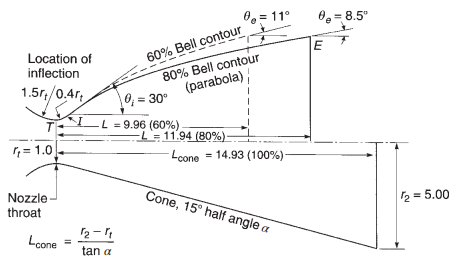
\includegraphics[width=0.82\linewidth]{Images/RPE.png}}{\IfFileExists{Images/RPE (1).png}{\includegraphics[width=0.82\linewidth]{Images/RPE (1).png}}{\fbox{\parbox{0.82\linewidth}{\centering Missing figure file: \texttt{RPE.png} or \texttt{RPE (1).png}}}}}
    \caption{Reference bell-nozzle proportions from the Sutton/Biblarz formulation.}
    \label{fig:RPE_geometry}
\end{figure}

\subsubsection{Global piecewise contour architecture}

The contour is constructed from four segments:
\begin{enumerate}
    \item initial straight converging line;
    \item subsonic circular arc upstream of the throat;
    \item supersonic circular arc immediately downstream of the throat;
    \item parabolic supersonic contour up to the exit plane.
\end{enumerate}

The coordinate origin is initially placed at the throat, with the nozzle axis along $x$ and the local radius along $r$. The throat point is therefore
\begin{equation}
(x_t,r_t)=(0,r_t).
\end{equation}

The full profile is later translated horizontally so that the exported and displayed geometry starts at $x=0$.

\subsubsection{Upstream throat-radius circular arc}

The subsonic circular arc uses a radius
\begin{equation}
R_{sub}=1.5r_t.
\end{equation}

Its center is placed on the radial axis at
\begin{equation}
C_{sub}=(0,2.5r_t).
\end{equation}

The circular equation is
\begin{equation}
x^2+(r-2.5r_t)^2=(1.5r_t)^2.
\end{equation}

The lower branch of the circle defines the desired arc:
\begin{equation}
r(x)=2.5r_t-\sqrt{(1.5r_t)^2-x^2},
\qquad x\in[x_r,0].
\label{eq:sub_arc}
\end{equation}

The connection point between the initial straight line and the subsonic arc is
\begin{align}
x_r &= -1.5r_t\sin(\theta_{sub}),
\label{eq:xr}\\
r_r &= 2.5r_t-1.5r_t\cos(\theta_{sub}).
\label{eq:yr}
\end{align}

\begin{figure}[H]
\centering
\begin{tikzpicture}[scale=1.75, line cap=round, line join=round]

% ---------------------------------------------------------
% Key points
% ---------------------------------------------------------
\coordinate (O) at (0,0);           % x=0 reference on x-axis
\coordinate (T) at (0,1.10);        % throat point
\coordinate (C) at (0,3.35);        % center of subsonic circle
\coordinate (Q) at (-1.299,1.85);   % connection point, on circle of radius 1.5

% ---------------------------------------------------------
% Axes
% ---------------------------------------------------------
\draw[black,
      dash pattern=on 8pt off 2pt on 1pt off 2pt,
      -latex] (-3.40,0) -- (1.80,0);    % x-axis
\draw[black,-latex] (0,-0.05) -- (0,4.35);      % vertical reference axis

% ---------------------------------------------------------
% Dashed construction lines
% ---------------------------------------------------------
\draw[densely dashed, gray] (Q) -- (Q |- O);      % vertical from Q to x-axis
\draw[densely dashed, gray] (Q) -- (0,1.85);      % horizontal from Q to y-axis
\draw[densely dashed, gray] (T) -- (O);           % vertical from throat to x-axis

% ---------------------------------------------------------
% Initial straight converging line
% ---------------------------------------------------------
\draw[black, line width=0.9pt] ($(Q)+(-1.75,1.75)$) -- (Q);

\draw[black, line width=0.9pt, -latex] (-3.5,0.75) -- (-2.25,0.75);

\draw[black, line width=0.9pt, -latex] (-3.5,1.05) -- (-2.25,1.05);

\draw[black, line width=0.9pt, -latex] (-3.5,0.9) -- (-2,0.9);

\node at (-2.675,1.2) {$\dot{m}_{\text{prop}}$};
% ---------------------------------------------------------
% Subsonic arc (lower branch of circle)
% Circle center C=(0,2.60), radius=1.5
% From Q to T
% ---------------------------------------------------------
\draw[black, line width=0.9pt]
    (Q) arc[start angle=210, end angle=270, radius=1.5];

% ---------------------------------------------------------
% Red auxiliary geometry
% ---------------------------------------------------------

% Horizontal reference through Q
\draw[red!70!black,dashed , line width=0.7pt] (-2.25,1.85) -- (Q);

% Radius from center to Q
\draw[red!70!black, dashed, line width=0.8pt] (C) -- (Q);

% Vertical reference from center downward
\draw[red!70!black, dashed, line width=0.8pt] (C) -- (0,1.10);

% ---------------------------------------------------------
% Point marker at Q
% ---------------------------------------------------------
\filldraw[white] (Q) circle (1.5pt);
\draw (Q) circle (2 pt);

% ---------------------------------------------------------
% Angle theta_sub at Q (between left horizontal and tangent line)
% ---------------------------------------------------------
\draw[black]
    ($(Q)+(-0.34,0)$) arc[start angle=180, end angle=135, radius=0.34];
\node[anchor=east] at ($(Q)+(-0.42,0.2)$) {$\theta_{\text{sub}}$};

% ---------------------------------------------------------
% Angle theta_sub at C (between downward vertical and radius CQ)
% ---------------------------------------------------------
\draw[red!70!black]
    ($(C)+(0,-0.42)$) arc[start angle=-90, end angle=-130, radius=0.42];
\node[anchor=west] at ($(C)+(-0.5,-0.74)$) { $\theta_{\text{sub}}$};

% ---------------------------------------------------------
% Radius label
% ---------------------------------------------------------
\node[anchor=west] at (-1.25,2.7) {$1.5r_t$};
\coordinate (F) at ($(Q)+(-1.75,1.75)$);

\draw[black, line width=0.9pt] (F) -- (Q);

\draw[densely dashed, gray] (F) -- (0,3.6);
\draw[densely dashed, gray] (F) -- (-1.299-1.75,0);


\node[anchor=west] at (0,3.6) {$r_{in}$};
% ---------------------------------------------------------
% Labels
% ---------------------------------------------------------
\node[anchor=north] at (-1.299,0) {$x_r$};
\node[anchor=north] at (0,0) { $0$};
\node[anchor=west]  at (0,1.85) {$y_r$};
\node[anchor=west]  at (0,4.35) { $y_r$};
\node[anchor=west]  at (T) { $r_t$};
\node[anchor=north] at (1.75,0) { $x$};
\node[below left=2pt] at (Q) {$Q$};
% ---------------------------------------------------------
% Q coordinate box
% ---------------------------------------------------------
\draw[black] (1.05,1.72) rectangle (2.80,2.25);
\node at (1.925,1.985) {$Q=(x_r,y_r)$};

\end{tikzpicture}
\caption{Subsonic geometric relations and definition of the converging arc.}
\label{fig:subsonic_geometry_tikz}
\end{figure}

\subsubsection{Linear converging-section approximation}

The initial converging section is approximated as a straight line tangent to the subsonic arc at $(x_r,r_r)$. Its slope is set by the angle $\theta_{sub}$:
\begin{equation}
m_{sub}=-\tan(\theta_{sub}).
\end{equation}

The line equation is
\begin{equation}
r(x)=m_{sub}x+b_{sub},
\end{equation}
where
\begin{equation}
b_{sub}=r_r-m_{sub}x_r.
\end{equation}

Substituting Eqs.~\eqref{eq:xr} and~\eqref{eq:yr}, the line can also be written as
\begin{equation}
r(x)=-\tan(\theta_{sub})x
+r_t\left[2.5-1.5\cos(\theta_{sub})-1.5\sin(\theta_{sub})\tan(\theta_{sub})\right].
\label{eq:line_expanded}
\end{equation}

The first axial coordinate $x_f$ is obtained from the chamber radius condition,
\begin{equation}
r(x_f)=r_c,
\end{equation}
which gives
\begin{equation}
x_f=\frac{r_c-b_{sub}}{m_{sub}} .
\label{eq:xf}
\end{equation}

The contraction ratio is then
\begin{equation}
CR=\frac{A_c}{A_t}=\frac{r_c^2}{r_t^2}.
\label{eq:contraction_ratio}
\end{equation}

\subsubsection{Downstream throat-radius circular arc}

Immediately downstream of the throat, the supersonic arc uses radius
\begin{equation}
R_{sup}=0.4r_t.
\end{equation}

Its center is placed at
\begin{equation}
C_{sup}=(0,1.4r_t).
\end{equation}

The circular equation is
\begin{equation}
x^2+(r-1.4r_t)^2=(0.4r_t)^2.
\end{equation}

The branch used for the nozzle profile is
\begin{equation}
r(x)=1.4r_t-\sqrt{(0.4r_t)^2-x^2},
\qquad x\in[0,x_P].
\label{eq:sup_arc}
\end{equation}

Equivalently, the arc can be parameterized by the angle $\theta$:
\begin{align}
x(\theta)&=0.4r_t\cos\theta,\\
r(\theta)&=1.4r_t-0.4r_t\sin\theta,
\end{align}
with
\begin{equation}
\theta\in\left[\frac{\pi}{2},\frac{\pi}{2}-\theta_{in}\right].
\end{equation}

The final point of the arc is the beginning of the parabolic contour:
\begin{align}
x_P &=0.4r_t\sin(\theta_{in}),
\label{eq:xP}\\
r_P &=1.4r_t-0.4r_t\cos(\theta_{in}).
\label{eq:yP}
\end{align}

\begin{figure}[H]
\centering
\begin{tikzpicture}[scale=1.75, line cap=round, line join=round]

% ---------------------------------------------------------
% Parameters
% ---------------------------------------------------------
\pgfmathsetmacro{\thetaInDeg}{35}
\pgfmathsetmacro{\Rsup}{0.80}      % schematic radius representing 0.4 rt
\pgfmathsetmacro{\Cy}{1.90}        % center of supersonic arc
\pgfmathsetmacro{\Ty}{\Cy-\Rsup}   % throat point y-coordinate

\pgfmathsetmacro{\Px}{\Rsup*sin(\thetaInDeg)}
\pgfmathsetmacro{\Py}{\Cy-\Rsup*cos(\thetaInDeg)}

\pgfmathsetmacro{\xE}{5.25}        % exit x-position (Lfinal)
\pgfmathsetmacro{\yE}{3.10}        % exit radius re

% Parabola coefficients:
% y(Px)=Py, y'(Px)=tan(theta_in), y(xE)=yE
\pgfmathsetmacro{\mP}{tan(\thetaInDeg)}
\pgfmathsetmacro{\den}{\xE-\Px}
\pgfmathsetmacro{\aPar}{(\yE-\Py-\mP*(\den))/(\den*\den)}
\pgfmathsetmacro{\bPar}{\mP-2*\aPar*\Px}
\pgfmathsetmacro{\cPar}{\Py-\aPar*\Px*\Px-\bPar*\Px}

\pgfmathsetmacro{\mE}{2*\aPar*\xE+\bPar}
\pgfmathsetmacro{\thetaOutDeg}{atan(\mE)}

% ---------------------------------------------------------
% Key points
% ---------------------------------------------------------
\coordinate (O) at (0,0);                    % x=0 reference
\coordinate (T) at (0,\Ty);                  % throat point
\coordinate (C) at (0,\Cy);                  % center of supersonic arc
\coordinate (P) at (\Px,\Py);                % transition point
\coordinate (E) at (\xE,\yE);                % nozzle exit point

% ---------------------------------------------------------
% Axes
% ---------------------------------------------------------
\draw[black,
      dash pattern=on 8pt off 2pt on 1pt off 2pt,
      -latex] (-0.25,0) -- (6.15,0);        % x-axis
\draw[black,-latex] (0,-0.05) -- (0,4.25);  % y-axis

% ---------------------------------------------------------
% Dashed construction lines
% ---------------------------------------------------------
\draw[densely dashed, gray] (P) -- (P |- O);     % vertical from P to x-axis
\draw[densely dashed, gray] (P) -- (0,\Py);      % horizontal from P to y-axis
\draw[densely dashed, gray] (E) -- (E |- O);     % vertical from exit to x-axis
\draw[densely dashed, gray] (E) -- (0, \yE);     % vertical from exit to x-axis

% ---------------------------------------------------------
% Supersonic arc (circular)
% ---------------------------------------------------------
\draw[black, line width=0.9pt]
    (T) arc[start angle=-90, end angle={-90+\thetaInDeg}, radius=\Rsup];

% ---------------------------------------------------------
% Parabolic divergent contour
% ---------------------------------------------------------
\draw[black, line width=0.9pt]
    plot[domain=\Px:\xE, samples=250]
    (\x,{\aPar*\x*\x+\bPar*\x+\cPar});

% ---------------------------------------------------------
% Red auxiliary geometry
% ---------------------------------------------------------

% Vertical reference from center to throat
\draw[red!70!black, dashed, line width=0.8pt] (C) -- (T);

% Radius from center to P
\draw[red!70!black, dashed, line width=0.8pt] (C) -- (P);

% Horizontal reference through P
\draw[red!70!black, dashed, line width=0.7pt] (P) -- ++(0.85,0);

% Small tangent reference at P
\draw[red!70!black, line width=0.7pt]
    ($(P)+(-0.15,-0.10)$) -- ++(\thetaInDeg:1.15);

% Exit tangent reference
\draw[red!70!black, line width=0.7pt]
    (E) -- ++(0.90,0);
\draw[red!70!black, line width=0.7pt]
    (E) -- ++(\thetaOutDeg:0.90);

% ---------------------------------------------------------
% Point marker at P
% ---------------------------------------------------------
\filldraw[white] (P) circle (1.5pt);
\draw (P) circle (2 pt);

% ---------------------------------------------------------
% Angle theta_in at P
% ---------------------------------------------------------
\draw[black]
    ($(P)+(0.34,0)$) arc[start angle=0, end angle=\thetaInDeg, radius=0.34];
\node[anchor=west] at ($(P)+(0.4,0.13)$) {$\theta_{\text{in}}$};

% ---------------------------------------------------------
% Angle theta_in at C
% ---------------------------------------------------------
\draw[red!70!black]
    ($(C)+(0,-0.42)$) arc[start angle=-90, end angle={-90+\thetaInDeg}, radius=0.42];
\node[anchor=west] at ($(C)+(0,-0.54)$) {$\theta_{\text{in}}$};

% ---------------------------------------------------------
% Angle theta_out at E
% ---------------------------------------------------------
\draw[red!70!black]
    ($(E)+(0.36,0)$) arc[start angle=0, end angle=\thetaOutDeg, radius=0.36];
\node[anchor=west] at ($(E)+(0.95,0.18)$) {$\theta_{\text{out}}$};


% ---------------------------------------------------------
% Radius label
% ---------------------------------------------------------
\node[anchor=west] at (0.15,1.65) {$0.4r_t$};

% ---------------------------------------------------------
% Labels
% ---------------------------------------------------------
\node[anchor=north] at (\Px,0) {$P_x$};
\node[anchor=north] at (0,0) {$0$};
\node[anchor=east]  at (0,\Py+0.1) {$P_y$};
\node[anchor=east] at ($(T)+(0,-0.1)$) {$r_t$};
\node[anchor=east]  at (0, \yE) {$r_e$};
\node[anchor=north] at (\xE,0) {$L_{\text{final}}$};
\node[anchor=west]  at (0,4.22) {$y$};
\node[anchor=north] at (6.10,0) {$x$};
\node[below right=1pt] at (P) {$P$};

% ---------------------------------------------------------
% P coordinate box
% ---------------------------------------------------------
\draw[black] (2.05,3.28) rectangle (3.80,3.81);
\node at (2.925,3.545) {$P=(P_x,P_y)$};

\draw[black, line width=0.9pt, -latex] (3,1.2) -- (4.5,1.2);

\draw[black, line width=0.9pt, -latex] (3,1.05) -- (4.75,1.05);

\draw[black, line width=0.9pt, -latex] (3,0.9) -- (4.5,0.9);

\node at (3.675,1.5) {$\dot{m}_{\text{prop}}$};

\end{tikzpicture}
\caption{Supersonic throat arc and transition into the parabolic diverging contour.}
\label{fig:supersonic_geometry_tikz}
\end{figure}

\subsubsection{Reference conical length and bell shortening factor}

The reference conical nozzle length is computed from the exit radius, throat radius and conical half-angle $\alpha$:
\begin{equation}
L_{cone}=\frac{r_e-r_t}{\tan\alpha}.
\label{eq:Lcone}
\end{equation}

The bell nozzle uses only a fraction $K_b$ of this length:
\begin{equation}
L_{parab}=K_b L_{cone}.
\label{eq:Lparab}
\end{equation}

The final axial coordinate of the parabolic section in the throat-centered coordinate system is
\begin{equation}
L=x_P+L_{parab}.
\label{eq:Lfinal}
\end{equation}

\subsubsection{Parabolic diverging-contour closure}

The parabolic contour is written as
\begin{equation}
r(x)=ax^2+bx+c,\qquad x\in[x_P,L].
\label{eq:parabola}
\end{equation}

A general parabola has three coefficients, so three independent conditions are imposed:
\begin{align}
r(x_P)&=r_P,
\label{eq:par_cond1}\\
r'(x_P)&=\tan(\theta_{in}),
\label{eq:par_cond2}\\
r(L)&=r_e.
\label{eq:par_cond3}
\end{align}

The first condition enforces positional continuity with the supersonic arc. The second condition enforces slope continuity and guarantees a smooth transition between the circular arc and the parabola. The third condition fixes the exit radius and therefore the desired expansion ratio.

The ideal case could also impose an exit angle condition,
\begin{equation}
r'(L)=\tan(\theta_{out}),
\end{equation}
but this would overdefine a simple parabola. Therefore, in the present formulation, $\theta_{out}$ is not prescribed; it is an output of the geometry.

The coefficient system is
\begin{equation}
\begin{bmatrix}
x_P^2 & x_P & 1\\
2x_P & 1 & 0\\
L^2 & L & 1
\end{bmatrix}
\begin{bmatrix}
a\\b\\c
\end{bmatrix}
=
\begin{bmatrix}
r_P\\ \tan(\theta_{in})\\ r_e
\end{bmatrix}.
\label{eq:parabola_matrix}
\end{equation}

Solving this linear system gives the parabolic coefficients that fully define the diverging section.

\subsubsection{Exit-plane wall angle}

The exit angle is obtained from the slope of the parabolic contour evaluated at the nozzle exit plane:
\begin{equation}
\theta_{out}=\arctan\left(2aL+b\right).
\label{eq:theta_out}
\end{equation}

This angle represents the local divergence of the flow at the nozzle exit and directly affects axial momentum efficiency. A large exit angle increases the radial velocity component and reduces useful axial thrust.

\subsubsection{Complete piecewise radius function}

Using the previous relations, the complete throat-centered nozzle contour can be written as
\begin{equation}
r(x)=
\begin{cases}
-\tan(\theta_{sub})x+b_{sub},
& x\in[x_f,x_r],\\[6pt]
2.5r_t-\sqrt{(1.5r_t)^2-x^2},
& x\in[x_r,0],\\[6pt]
1.4r_t-\sqrt{(0.4r_t)^2-x^2},
& x\in[0,x_P],\\[6pt]
ax^2+bx+c,
& x\in[x_P,L].
\end{cases}
\label{eq:piecewise_nozzle}
\end{equation}

This equation is one of the most important outputs of the geometric formulation because it gives a continuous mathematical representation of the entire nozzle contour.

% =========================================================
\subsubsection{Geometric station and angle summary}
% =========================================================

An illustrative nozzle geometry corresponding to $\varepsilon=5.0$ and $r_t=\SI{0.020}{m}$ is presented in Fig.~\ref{fig:nozzle_piecewise_tikz} to identify the stations and angles introduced in the previous sections.

\begin{figure}[H]
\centering
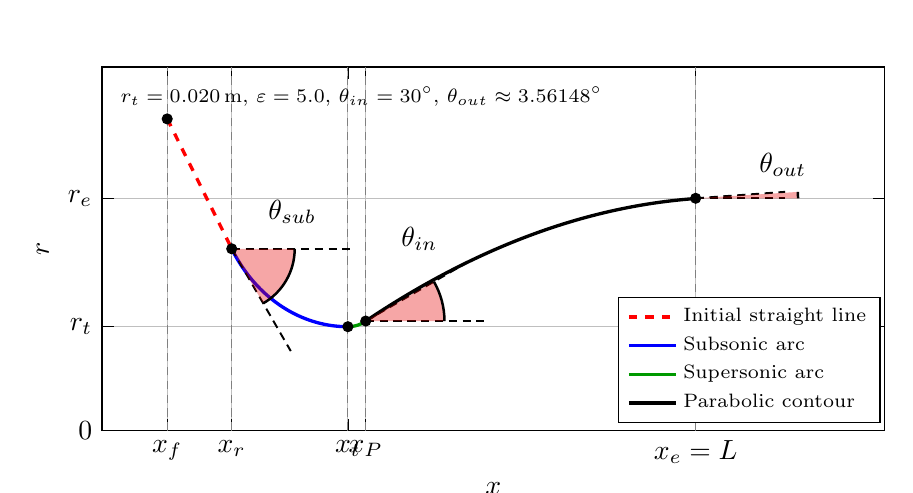
\begin{tikzpicture}
\begin{axis}[
    width=0.95\linewidth,
    height=6.2cm,
    grid=both,
    xlabel={$x$},
    ylabel={$r$},
    xmin=0, xmax=0.175,
    ymin=0, ymax=0.07,
    trig format=deg,
    scaled ticks=false,
    tick style={black},
    legend style={at={(0.995,0.02)},anchor=south east,fill=white,draw=black,line width=0.4pt,font=\scriptsize},
    legend cell align=left,
]

\pgfmathsetmacro{\rt}{0.020}
\pgfmathsetmacro{\eps}{5.0}
\pgfmathsetmacro{\re}{sqrt(\eps)*\rt}
\pgfmathsetmacro{\alphaDeg}{15}
\pgfmathsetmacro{\bell}{0.80}
\pgfmathsetmacro{\thetaSubDeg}{60}
\pgfmathsetmacro{\thetaInDeg}{30}
\pgfmathsetmacro{\Rch}{0.060}
\pgfmathsetmacro{\tx}{0.055}

\pgfmathsetmacro{\xr}{-1.5*\rt*sin(\thetaSubDeg)}
\pgfmathsetmacro{\yr}{2.5*\rt - 1.5*\rt*cos(\thetaSubDeg)}
\pgfmathsetmacro{\xR}{\tx+\xr}
\pgfmathsetmacro{\mLine}{-tan(\thetaSubDeg)}
\pgfmathsetmacro{\bLine}{\yr - \mLine*\xr}
\pgfmathsetmacro{\xf}{(\Rch - \bLine)/\mLine}
\pgfmathsetmacro{\xF}{\tx+\xf}

\pgfmathsetmacro{\rSup}{0.4*\rt}
\pgfmathsetmacro{\Px}{\rSup*sin(\thetaInDeg)}
\pgfmathsetmacro{\Py}{1.4*\rt - \rSup*cos(\thetaInDeg)}
\pgfmathsetmacro{\xP}{\tx+\Px}

\pgfmathsetmacro{\Lcone}{(\re-\rt)/tan(\alphaDeg)}
\pgfmathsetmacro{\L}{\Px + \bell*\Lcone}
\pgfmathsetmacro{\xE}{\tx+\L}
\pgfmathsetmacro{\mZero}{tan(\thetaInDeg)}
\pgfmathsetmacro{\den}{(\L-\Px)}
\pgfmathsetmacro{\aPar}{(\re - \Py - \mZero*(\den))/(\den*\den)}
\pgfmathsetmacro{\bPar}{\mZero - 2*\aPar*\Px}
\pgfmathsetmacro{\cPar}{\Py - \aPar*\Px*\Px - \bPar*\Px}
\pgfmathsetmacro{\thetaOutDeg}{atan(2*\aPar*\L + \bPar)}
\pgfmathsetmacro{\mOut}{tan(\thetaOutDeg)}

\pgfplotsset{
  xtick={\xF,\xR,\tx,\xP,\xE},
  xticklabels={$x_f$,$x_r$,$x_t$,$x_P$,$x_e=L$},
  ytick={0,\rt,\re},
  yticklabels={$0$,$r_t$,$r_e$},
}

\addplot[dashed, very thick, red, domain=\xF:\xR, samples=2] ({x},{\mLine*(x-\tx)+\bLine});
\addlegendentry{Initial straight line}

\addplot[very thick, blue, domain=\xR:\tx, samples=250] ({x},{2.5*\rt - sqrt((1.5*\rt)^2 - (x-\tx)^2)});
\addlegendentry{Subsonic arc}

\addplot[very thick, green!60!black, domain=\tx:\xP, samples=250] ({x},{1.4*\rt - sqrt((0.4*\rt)^2 - (x-\tx)^2)});
\addlegendentry{Supersonic arc}

\addplot[very thick, black, domain=\xP:\xE, samples=350] ({x},{\aPar*(x-\tx)^2 + \bPar*(x-\tx) + \cPar});
\addlegendentry{Parabolic contour}

\addplot[only marks, mark=*, mark size=1.8pt] coordinates {(\xF,\Rch) (\xR,\yr) (\tx,\rt) (\xP,\Py) (\xE,\re)};

\addplot[densely dashed, gray] coordinates {(\xF,0) (\xF,0.07)};
\addplot[densely dashed, gray] coordinates {(\xR,0) (\xR,0.07)};
\addplot[densely dashed, gray] coordinates {(\tx,0) (\tx,0.07)};
\addplot[densely dashed, gray] coordinates {(\xP,0) (\xP,0.07)};
\addplot[densely dashed, gray] coordinates {(\xE,0) (\xE,0.07)};

\path (axis cs:\xR,\yr) coordinate (Rpt);
\path (axis cs:\xP,\Py) coordinate (Ppt);
\path (axis cs:\xE,\re) coordinate (Ept);

\tikzset{angline/.style={densely dashed, black, line width=0.7pt}}

\def\Lsub{15mm}
\def\RadFillSub{8mm}
\def\RadArcSub{8mm}
\pgfmathsetmacro{\phiSub}{\thetaSubDeg}
\draw[angline] (Rpt) -- ++(\Lsub,0);
\draw[angline] (Rpt) -- ++(-\phiSub:\Lsub);
\fill[red!90!black, opacity=0.35] (Rpt) -- ++(\RadFillSub,0) arc[start angle=0, end angle=-\phiSub, radius=\RadFillSub] -- cycle;
\draw[black, line width=0.9pt] (Rpt) ++(\RadArcSub,0) arc[start angle=0, end angle=-\phiSub, radius=\RadArcSub];
\node[anchor=south west] at (axis cs:\xR+0.006,\yr+0.003) {$\theta_{sub}$};

\def\Lin{15mm}
\def\RadFillIn{10mm}
\def\RadArcIn{10mm}
\pgfmathsetmacro{\phiIn}{\thetaInDeg}
\draw[angline] (Ppt) -- ++(\Lin,0);
\draw[angline] (Ppt) -- ++(\phiIn:\Lin);
\fill[red!90!black, opacity=0.35] (Ppt) -- ++(\RadFillIn,0) arc[start angle=0, end angle=\phiIn, radius=\RadFillIn] -- cycle;
\draw[black, line width=0.9pt] (Ppt) ++(\RadArcIn,0) arc[start angle=0, end angle=\phiIn, radius=\RadArcIn];
\node[anchor=north] at (axis cs:\xP+0.012,\Py+0.02) {$\theta_{in}$};

\pgfmathsetmacro{\dxE}{0.020}
\draw[angline] (axis cs:\xE,\re) -- (axis cs:\xE+\dxE,\re);
\pgfmathsetmacro{\dyE}{\mOut*\dxE}
\draw[angline] (axis cs:\xE,\re) -- (axis cs:\xE+\dxE,\re+\dyE);
\pgfmathsetmacro{\phiOut}{\thetaOutDeg}
\def\RadFill{13mm}
\def\RadArc{13mm}
\path (Ept) ++(\RadFill,0) coordinate (FillStart);
\fill[red!90!black, opacity=0.35] (Ept) -- (FillStart) arc[start angle=0, end angle=\phiOut, radius=\RadFill] -- cycle;
\path (Ept) ++(\RadArc,0) coordinate (ArcStart);
\draw[black, line width=0.9pt] (ArcStart) arc[start angle=0, end angle=\phiOut, radius=\RadArc];
\node[anchor=center] at (rel axis cs:0.87,0.73) {$\theta_{out}$};

\node[anchor=north west] at (axis cs:0.002,0.068) {\scriptsize $r_t=\rt\,\mathrm{m}$, $\varepsilon=\eps$, $\theta_{in}=\thetaInDeg^\circ$, $\theta_{out}\approx\thetaOutDeg^\circ$};

\end{axis}
\end{tikzpicture}
\caption{Two-dimensional nozzle contour with region definitions, stations and angle notation.}
\label{fig:nozzle_piecewise_tikz}
\end{figure}

% =========================================================
\subsection{Numerical Coordinate Conditioning and Two-Dimensional Contour Output}
% =========================================================


\subsubsection{Axial coordinate translation}

The throat-centered coordinate system is convenient for mathematical construction, but it produces negative $x$ values in the subsonic converging section. For plotting, CAD export and easier interpretation, the profile is translated horizontally so that the first point of the nozzle starts at $x=0$.

The required translation is
\begin{equation}
\Delta x=-x_f.
\label{eq:translation_simple}
\end{equation}

Using the line geometry, this can also be written as
\begin{equation}
\Delta x=-x_r+\frac{r_c-y_r}{\tan(\theta_{sub})}.
\label{eq:translation}
\end{equation}

\begin{figure}[H]
\centering
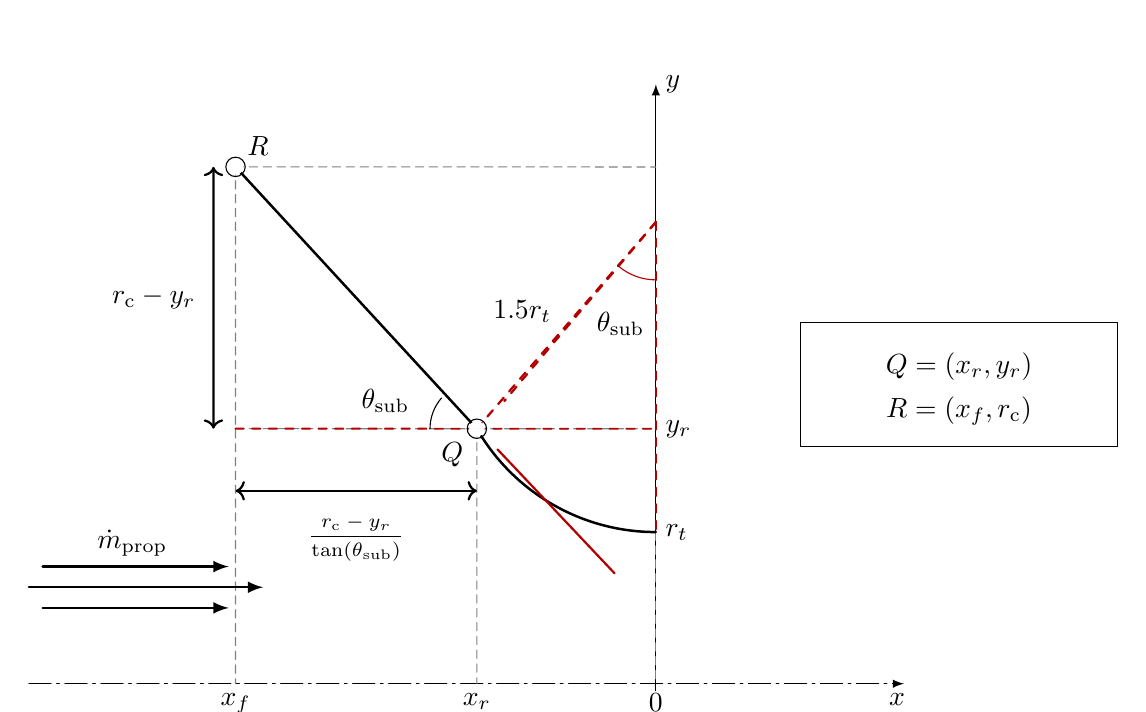
\begin{tikzpicture}[scale=1.75, line cap=round, line join=round]

% ---------------------------------------------------------
% Key points
% ---------------------------------------------------------
\coordinate (O) at (0,0);            % x = 0 reference
\coordinate (T) at (0,1.10);         % throat point
\coordinate (C) at (0,3.35);         % center of subsonic circle
\coordinate (Q) at (-1.299,1.85);    % connection point
\coordinate (R) at (-3.05,3.75);     % inlet point: R=(xf,rchamber)

% Auxiliary points
\coordinate (Rf) at (R |- O);        % projection of R on x-axis
\coordinate (Rq) at (R |- Q);        % point at x=xf and y=yr
\coordinate (Qf) at (Q |- O);        % projection of Q on x-axis

% ---------------------------------------------------------
% Axes
% ---------------------------------------------------------
\draw[black,
      dash pattern=on 8pt off 2pt on 1pt off 2pt,
      -latex] (-4.55,0) -- (1.80,0);

\draw[black,-latex] (0,-0.05) -- (0,4.35);

% ---------------------------------------------------------
% Dashed construction lines
% ---------------------------------------------------------

% Projections of Q
\draw[densely dashed, gray] (Q) -- (Qf);
\draw[densely dashed, gray] (Q) -- (0,1.85);

% Projection of throat
\draw[densely dashed, gray] (T) -- (O);

% Projections of R
\draw[densely dashed, gray] (R) -- (Rf);
\draw[densely dashed, gray] (R) -- (0,3.75);

% Horizontal level y_r extended to x_f
\draw[densely dashed, gray] (Rq) -- (Q);

% ---------------------------------------------------------
% Initial straight converging line
% ---------------------------------------------------------
\draw[black, line width=0.9pt] (R) -- (Q);

% ---------------------------------------------------------
% Mass-flow arrows
% ---------------------------------------------------------
\draw[black, line width=0.9pt, -latex] (-4.45,0.55) -- (-3.10,0.55);
\draw[black, line width=0.9pt, -latex] (-4.45,0.85) -- (-3.10,0.85);
\draw[black, line width=0.9pt, -latex] (-4.55,0.70) -- (-2.85,0.70);

\node at (-3.80,1.02) {$\dot{m}_{\text{prop}}$};

% ---------------------------------------------------------
% Subsonic arc
% ---------------------------------------------------------
\draw[black, line width=0.9pt]
    (Q) arc[start angle=210, end angle=270, radius=1.5];

% ---------------------------------------------------------
% Red auxiliary geometry
% ---------------------------------------------------------

% Horizontal reference through Q
\draw[red!70!black, dashed, line width=0.7pt] (Rq) -- (Q);
\draw[red!70!black, dashed, line width=0.7pt] (Q) -- (0,1.85);

% Radius from center to Q
\draw[red!70!black, dashed, line width=0.8pt] (C) -- (Q);

% Vertical reference from center downward
\draw[red!70!black, dashed, line width=0.8pt] (C) -- (0,1.10);

% Tangent-like auxiliary line at Q
\draw[red!70!black, line width=0.8pt]
    ($(Q)+(0.15,-0.15)$) -- ($(Q)+(1.00,-1.05)$);

% Extra construction line for upper angle
\draw[red!70!black, dashed, line width=0.8pt] (C) -- ++(-1.10,-1.30);

% ---------------------------------------------------------
% Vertical distance rchamber - yr
% ---------------------------------------------------------
\draw[black, <->, line width=0.8pt]
    ($(Rq)+(-0.16,0)$) -- ($(R)+(-0.16,0)$);

\node[anchor=east] at ($(Rq)!0.5!(R)+(-0.22,0)$)
    {$r_{\text{c}}-y_r$};

% ---------------------------------------------------------
% Horizontal distance dimension between x_f and x_r
% ---------------------------------------------------------
\draw[black, <->, line width=0.8pt]
    (-3.05,1.4) -- (-1.299,1.4);

\node[anchor=south] at ($(Rf)!0.5!(Qf)+(0,0.82)$)
    {\scriptsize $\dfrac{r_{\text{c}}-y_r}{\tan(\theta_{\text{sub}})}$};

% ---------------------------------------------------------
% Point marker at Q
% ---------------------------------------------------------
\filldraw[white] (Q) circle (1.5pt);
\draw (Q) circle (2 pt);

\filldraw[white] (R) circle (1.5pt);
\draw (R) circle (2 pt);

% ---------------------------------------------------------
% Angle theta_sub at Q
% ---------------------------------------------------------
\draw[black]
    ($(Q)+(-0.34,0)$) arc[start angle=180, end angle=139, radius=0.34];

\node[anchor=east] at ($(Q)+(-0.42,0.20)$)
    {$\theta_{\text{sub}}$};

% ---------------------------------------------------------
% Angle theta_sub at C
% ---------------------------------------------------------
\draw[red!70!black]
    ($(C)+(0,-0.42)$) arc[start angle=-90, end angle=-130, radius=0.42];

\node[anchor=west] at ($(C)+(-0.50,-0.74)$)
    {$\theta_{\text{sub}}$};

% ---------------------------------------------------------
% Radius label
% ---------------------------------------------------------
\node[anchor=west] at (-1.25,2.70) {$1.5r_t$};

% ---------------------------------------------------------
% Labels
% ---------------------------------------------------------
\node[anchor=north] at (-3.05,0) {$x_f$};
\node[anchor=north] at (-1.299,0) {$x_r$};
\node[anchor=north] at (0,0) {$0$};

\node[anchor=west] at (0,1.85) {$y_r$};
\node[anchor=west] at (0,1.10) {$r_t$};
\node[anchor=west] at (0,4.35) {$y$};
\node[anchor=north] at (1.75,0) {$x$};

\node[above right=1pt] at (R) {$R$};
\node[below left=2pt] at (Q) {$Q$};

% ---------------------------------------------------------
% Q/R coordinate box
% ---------------------------------------------------------
\draw[black] (1.05,1.72) rectangle (3.35,2.62);

\node at (2.20,2.30) {$Q=(x_r,y_r)$};
\node at (2.20,1.98) {$R=(x_f,r_{\text{c}})$};

\end{tikzpicture}
\caption{Horizontal translation used to move the nozzle start to $x=0$.}
\label{fig:translation_geometry_tikz}
\end{figure}


\clearpage
\begin{landscape}
\thispagestyle{plain}

\noindent
After translation, all axial coordinates become
\begin{equation}
\bar{x}=x+\Delta x.
\end{equation}

\noindent
The translated domain is
\begin{equation}
\bar{x}\in[0,L-x_f].
\end{equation}


\begin{center}
\noindent
\makebox[\linewidth][c]{%
\resizebox{0.95\linewidth}{!}{%
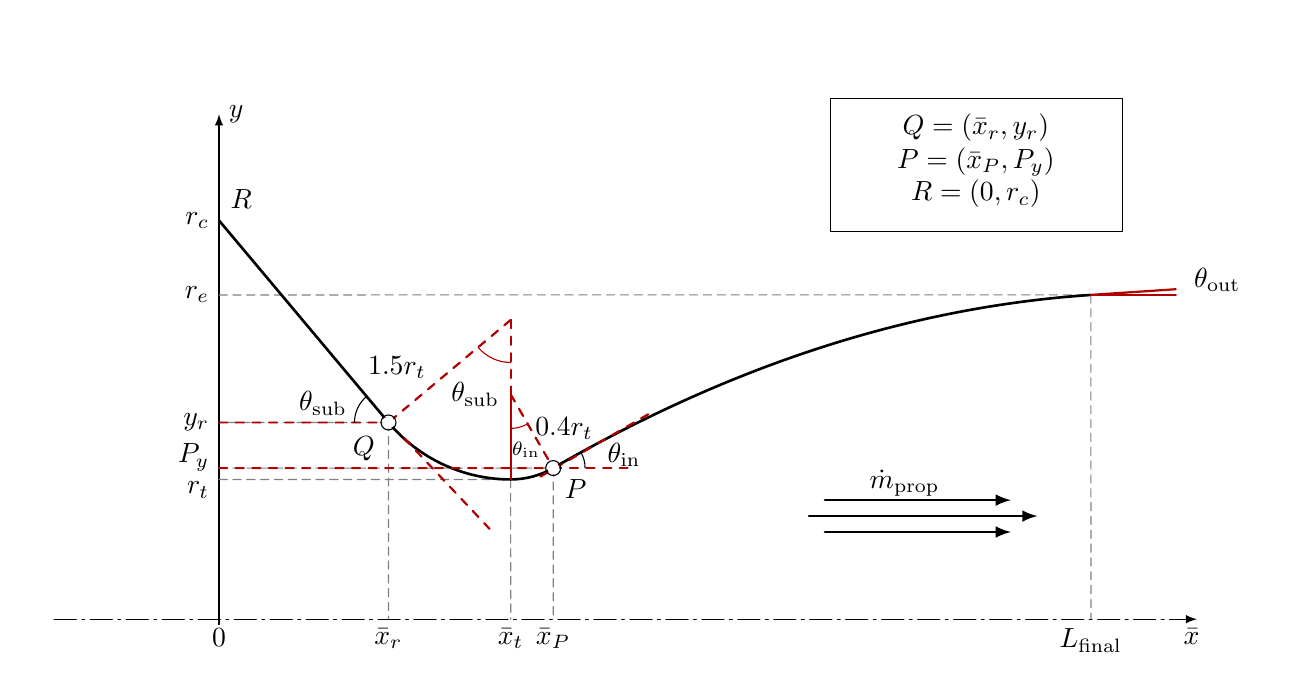
\begin{tikzpicture}[scale=1.35, line cap=round, line join=round]

% Optional bounding box to improve page centering
\path[use as bounding box] (-1.8,-0.8) rectangle (9.8,5.2);

% ---------------------------------------------------------
% Geometric parameters (schematic, but consistent)
% ---------------------------------------------------------
\pgfmathsetmacro{\thetaSubDeg}{50}
\pgfmathsetmacro{\thetaInDeg}{30}

\pgfmathsetmacro{\rch}{3.75}      % chamber radius
\pgfmathsetmacro{\yr}{1.85}       % y_r
\pgfmathsetmacro{\Rsub}{1.50}     % subsonic arc radius = 1.5 r_t
\pgfmathsetmacro{\Rsup}{0.80}     % supersonic arc radius = 0.4 r_t (schematic)

% Translated domain: nozzle starts at x = 0
\pgfmathsetmacro{\xrbar}{(\rch-\yr)/tan(\thetaSubDeg)}
\pgfmathsetmacro{\xtbar}{\xrbar+\Rsub*sin(\thetaSubDeg)}       % translated x_t

% Subsonic circle center and throat radius
\pgfmathsetmacro{\yCsub}{\yr+\Rsub*cos(\thetaSubDeg)}
\pgfmathsetmacro{\rt}{\yCsub-\Rsub}

% Supersonic arc
\pgfmathsetmacro{\yCsup}{\rt+\Rsup}
\pgfmathsetmacro{\xPbar}{\xtbar+\Rsup*sin(\thetaInDeg)}
\pgfmathsetmacro{\Py}{\yCsup-\Rsup*cos(\thetaInDeg)}

% Exit point
\pgfmathsetmacro{\xE}{8.20}
\pgfmathsetmacro{\re}{3.05}

% Parabola through P with slope theta_in and passing through exit
\pgfmathsetmacro{\mP}{tan(\thetaInDeg)}
\pgfmathsetmacro{\den}{\xE-\xPbar}
\pgfmathsetmacro{\aPar}{(\re-\Py-\mP*(\den))/(\den*\den)}
\pgfmathsetmacro{\bPar}{\mP-2*\aPar*\xPbar}
\pgfmathsetmacro{\cPar}{\Py-\aPar*\xPbar*\xPbar-\bPar*\xPbar}

% Exit slope / angle
\pgfmathsetmacro{\mE}{2*\aPar*\xE+\bPar}
\pgfmathsetmacro{\thetaOutDeg}{atan(\mE)}

% ---------------------------------------------------------
% Key points
% ---------------------------------------------------------
\coordinate (O) at (0,0);
\coordinate (R) at (0,\rch);                  % translated inlet point
\coordinate (Q) at (\xrbar,\yr);              % line-arc connection
\coordinate (T) at (\xtbar,\rt);              % throat
\coordinate (Csub) at (\xtbar,\yCsub);        % subsonic arc center
\coordinate (Csup) at (\xtbar,\yCsup);        % supersonic arc center
\coordinate (P) at (\xPbar,\Py);              % arc-parabola transition
\coordinate (E) at (\xE,\re);                 % exit point

% Projections
\coordinate (Qf) at (Q |- O);
\coordinate (Tf) at (T |- O);
\coordinate (Pf) at (P |- O);
\coordinate (Ef) at (E |- O);

% ---------------------------------------------------------
% Axes
% ---------------------------------------------------------
\draw[black,
      dash pattern=on 8pt off 2pt on 1pt off 2pt,
      -latex] (-1.55,0) -- (9.20,0);

\draw[black,-latex] (0,-0.05) -- (0,4.75);

% ---------------------------------------------------------
% Dashed construction lines
% ---------------------------------------------------------
\draw[densely dashed, gray] (Q) -- (Qf);
\draw[densely dashed, gray] (Q) -- (0,\yr);

\draw[densely dashed, gray] (T) -- (Tf);
\draw[densely dashed, gray] (0,\rt) -- (T);

\draw[densely dashed, gray] (P) -- (Pf);
\draw[densely dashed, gray] (0,\Py) -- (P);

\draw[densely dashed, gray] (E) -- (Ef);
\draw[densely dashed, gray] (0,\re) -- (E);

\draw[densely dashed, gray] (R) -- (0,\rch);

% ---------------------------------------------------------
% Mass-flow arrows
% ---------------------------------------------------------
\draw[black, line width=0.9pt, -latex] (5.70,0.82) -- (7.45,0.82);
\draw[black, line width=0.9pt, -latex] (5.70,1.12) -- (7.45,1.12);
\draw[black, line width=0.9pt, -latex] (5.55,0.97) -- (7.70,0.97);
\node at (6.45,1.28) {$\dot{m}_{\text{prop}}$};

% ---------------------------------------------------------
% Contour: straight line + subsonic arc + supersonic arc + parabola
% ---------------------------------------------------------

% Initial straight converging line
\draw[black, line width=0.95pt] (R) -- (Q);

% Subsonic arc
\draw[black, line width=0.95pt]
    (Q) arc[start angle={270-\thetaSubDeg}, end angle=270, radius=\Rsub];

% Supersonic arc
\draw[black, line width=0.95pt]
    (T) arc[start angle=-90, end angle={-90+\thetaInDeg}, radius=\Rsup];

% Parabolic divergent contour
\draw[black, line width=0.95pt]
    plot[domain=\xPbar:\xE, samples=250]
    (\x,{\aPar*\x*\x+\bPar*\x+\cPar});

% ---------------------------------------------------------
% Red auxiliary geometry: subsonic
% ---------------------------------------------------------

% Horizontal reference through Q
\draw[red!70!black, dashed, line width=0.7pt] (0,\yr) -- (Q);

% Radius from subsonic center to Q
\draw[red!70!black, dashed, line width=0.8pt] (Csub) -- (Q);

% Vertical reference from subsonic center to throat
\draw[red!70!black, dashed, line width=0.8pt] (Csub) -- (T);

% Tangent-like auxiliary line at Q
\draw[red!70!black,dashed, line width=0.8pt]
    ($(Q)+(0.15,-0.15)$) -- ($(Q)+(0.95,-1.00)$);

% Angle theta_sub at Q
\draw[black]
    ($(Q)+(-0.32,0)$) arc[start angle=180, end angle={180-\thetaSubDeg}, radius=0.32];
\node[anchor=east] at ($(Q)+(-0.30,0.18)$) {$\theta_{\text{sub}}$};

% Angle theta_sub at subsonic center
\draw[red!70!black]
    ($(Csub)+(0,-0.40)$) arc[start angle=-90, end angle={-90-\thetaSubDeg}, radius=0.40];
\node[anchor=west] at ($(Csub)+(-0.65,-0.70)$) {$\theta_{\text{sub}}$};

% Subsonic radius label
\node[anchor=west] at ($(Csub)!0.55!(Q)+(-0.8,0.08)$) {$1.5r_t$};

% ---------------------------------------------------------
% Red auxiliary geometry: supersonic
% ---------------------------------------------------------

% Vertical reference from supersonic center to throat
\draw[red!70!black, dashed, line width=0.8pt] (Csup) -- (T);

% Radius from supersonic center to P
\draw[red!70!black, dashed, line width=0.8pt] (Csup) -- (P);

% Horizontal reference through P
\draw[red!70!black, dashed, line width=0.7pt] (0,\Py) -- (P);
\draw[red!70!black, dashed, line width=0.7pt] (P) -- ++(0.70,0);

% Tangent at P
\draw[red!70!black,dashed, line width=0.8pt]
    ($(P)+(-0.12,-0.08)$) -- ++(\thetaInDeg:1.20);

% Exit tangent references
\draw[red!70!black, line width=0.8pt] (E) -- ++(0.80,0);
\draw[red!70!black, line width=0.8pt] (E) -- ++(\thetaOutDeg:0.80);

% Angle theta_in at P
\draw[black]
    ($(P)+(0.30,0)$) arc[start angle=0, end angle=\thetaInDeg, radius=0.30];
\node[anchor=west] at ($(P)+(0.42,0.12)$) {$\theta_{\text{in}}$};

% Angle theta_in at supersonic center
\draw[red!70!black]
    ($(Csup)+(0,-0.32)$) arc[start angle=-90, end angle={-90+\thetaInDeg}, radius=0.32];
\node[anchor=west] at ($(Csup)+(-0.08,-0.52)$) {\scriptsize$\theta_{\text{in}}$};

% Angle theta_out at exit
\draw[red!70!black]
    ($(E)+(0.32,0)$) arc[start angle=0, end angle=\thetaOutDeg, radius=0.32];
\node[anchor=west] at ($(E)+(0.88,0.14)$) {$\theta_{\text{out}}$};

% Supersonic radius label
\node[anchor=west] at ($(Csup)!0.55!(P)+(-0.08,0.06)$) {$0.4r_t$};

% ---------------------------------------------------------
% Point markers
% ---------------------------------------------------------
\filldraw[white] (Q) circle (1.5pt);
\draw (Q) circle (2pt);

\filldraw[white] (P) circle (1.5pt);
\draw (P) circle (2pt);

% ---------------------------------------------------------
% Labels
% ---------------------------------------------------------
\node[above right=1pt] at (R) {$R$};
\node[below left=2pt] at (Q) {$Q$};
\node[below right=1pt] at (P) {$P$};

\node[anchor=north] at (0,0) {$0$};
\node[anchor=north] at (\xrbar,0) {$\bar{x}_r$};
\node[anchor=north] at (\xtbar,0) {$\bar{x}_t$};
\node[anchor=north] at (\xPbar,0) {$\bar{x}_P$};
\node[anchor=north] at (\xE,0) {$L_{\text{final}}$};

\node[anchor=east] at (0,\rch) {$r_c$};
\node[anchor=east] at (0,\yr) {$y_r$};
\node[anchor=east] at (0,\rt-0.1) {$r_t$};
\node[anchor=east] at (0,\Py+0.1) {$P_y$};
\node[anchor=east] at (0,\re) {$r_e$};

\node[anchor=west] at (0,4.75) {$y$};
\node[anchor=north] at (9.15,0) {$\bar{x}$};

% ---------------------------------------------------------
% Coordinate box
% ---------------------------------------------------------
\draw[black] (5.75,3.65) rectangle (8.5,4.9);
\node at (7.12,4.62) {$Q=(\bar{x}_r,y_r)$};
\node at (7.12,4.30) {$P=(\bar{x}_P,P_y)$};
\node at (7.12,4.0) {$R=(0,r_c)$};

\end{tikzpicture}%
}%
}

\vspace{0.45cm}

\captionof{figure}{Combined translated nozzle contour showing the straight converging section, the subsonic throat arc, the supersonic throat arc, and the parabolic diverging section in the translated domain.}
\label{fig:combined_translated_nozzle_tikz}
\end{center}


\end{landscape}
\clearpage

\subsubsection{Derived geometric outputs}

The simulator outputs several secondary quantities that help evaluate the geometry:
\begin{align}
CR &= \frac{r_c^2}{r_t^2},\\
\varepsilon &= \frac{r_e^2}{r_t^2},\\
L_{nozzle} &= L-x_f,\\
\theta_{out} &= \arctan(2aL+b).
\end{align}

These quantities are displayed together with the two-dimensional profile to make each generated geometry immediately interpretable.

\begin{figure}[H]
    \centering
    \IfFileExists{Images/plot2D.png}{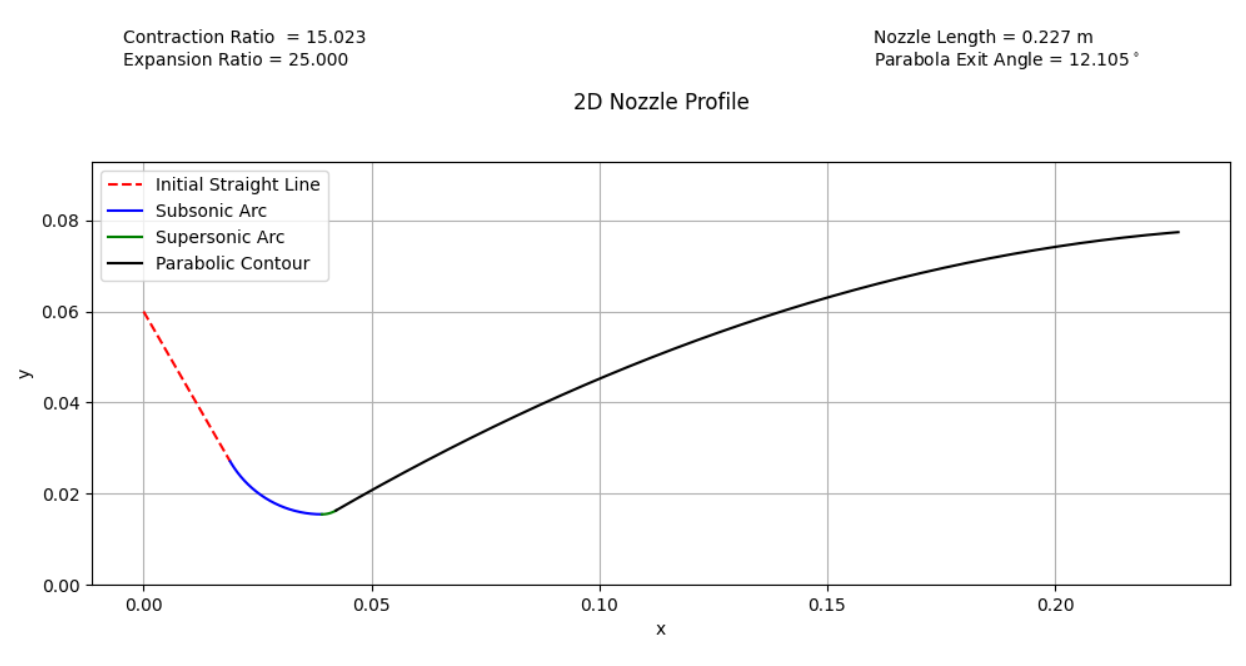
\includegraphics[width=0.85\linewidth]{Images/plot2D.png}}{\fbox{\parbox{0.78\linewidth}{\centering Missing figure file: \texttt{plot2D.png}}}}
    \caption{Example 1 of a generated two-dimensional nozzle geometry profile.}
    \label{fig:plot2D_example_2}
\end{figure}

\begin{figure}[H]
    \centering
    \IfFileExists{Images/ex3.png}{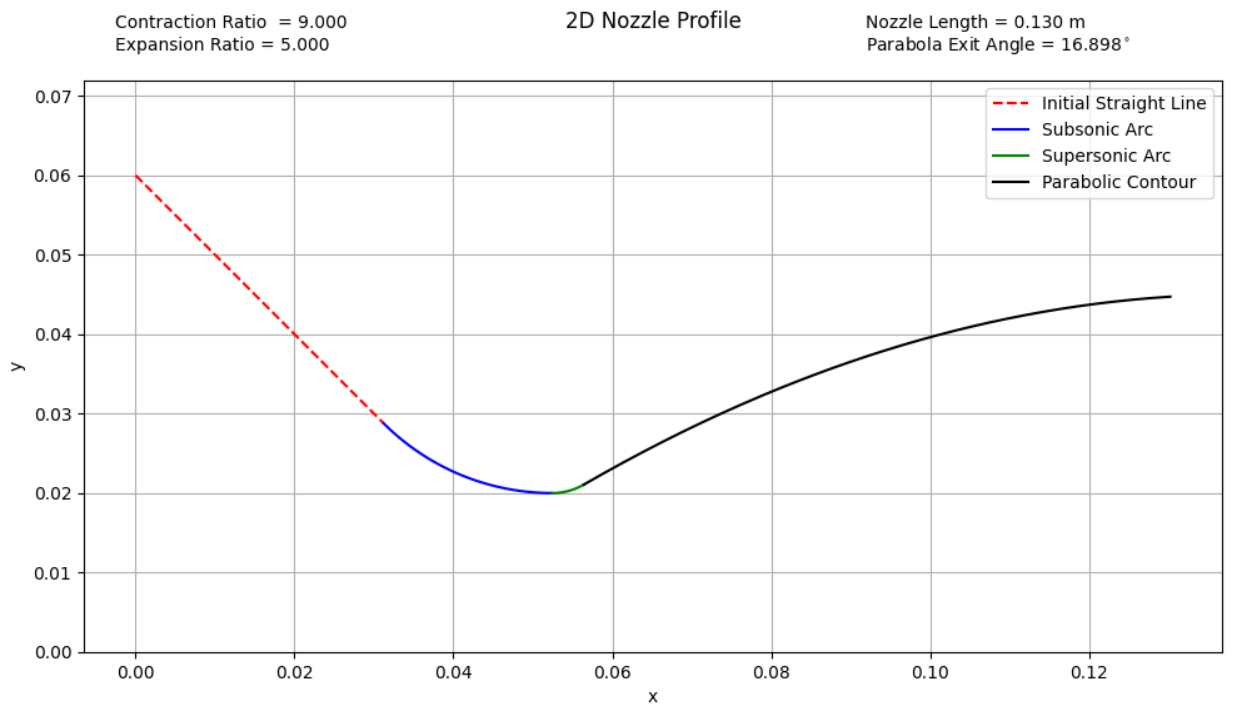
\includegraphics[width=0.85\linewidth]{Images/ex3.png}}{\fbox{\parbox{0.78\linewidth}{\centering Missing figure file: \texttt{plot2D.png}}}}
    \caption{Example 2 of a generated two-dimensional nozzle geometry profile.}
    \label{fig:plot2D}
\end{figure}

\newpage
% =========================================================
\subsection{Axisymmetric Three-Dimensional Geometry Reconstruction}
% =========================================================

\subsubsection{Surface-of-revolution definition}

Because the nozzle is axisymmetric, the three-dimensional surface is generated by revolving the two-dimensional radius function around the nozzle axis. For each axial coordinate $x_i$ and radius $r_i$, a circular ring is generated using the angular coordinate $\phi$:
\begin{align}
X_i(\phi)&=x_i,\\
Y_i(\phi)&=r_i\cos\phi,\\
Z_i(\phi)&=r_i\sin\phi,
\end{align}
with
\begin{equation}
\phi\in[0,2\pi].
\end{equation}

The complete nozzle surface is therefore
\begin{equation}
\bm{S}(x,\phi)=
\begin{bmatrix}
x\\
r(x)\cos\phi\\
r(x)\sin\phi
\end{bmatrix}.
\label{eq:surface_of_revolution}
\end{equation}

This formulation is important because it makes clear that the three-dimensional geometry is not an independent model. It is the direct revolution of the piecewise two-dimensional contour from Eq.~\eqref{eq:piecewise_nozzle}.



\subsubsection{Structured mesh matrices for visualization}

For numerical visualization, the axial and angular coordinates are assembled into matrices. If
\begin{equation}
\bm{x}=\begin{bmatrix}x_0&x_1&\cdots&x_n\end{bmatrix}^T,
\end{equation}
and
\begin{equation}
\bm{\phi}=\begin{bmatrix}\phi_0&\phi_1&\cdots&\phi_m\end{bmatrix},
\end{equation}
then the axial mesh has the structure
\begin{equation}
X=\begin{bmatrix}
x_0&x_0&\cdots&x_0\\
x_1&x_1&\cdots&x_1\\
\vdots&\vdots&\ddots&\vdots\\
x_n&x_n&\cdots&x_n
\end{bmatrix}.
\label{eq:Xmesh}
\end{equation}

The angular mesh is
\begin{equation}
\Phi=\begin{bmatrix}
\phi_0&\phi_1&\cdots&\phi_m\\
\phi_0&\phi_1&\cdots&\phi_m\\
\vdots&\vdots&\ddots&\vdots\\
\phi_0&\phi_1&\cdots&\phi_m
\end{bmatrix}.
\label{eq:Phimesh}
\end{equation}

The radial mesh is
\begin{equation}
R=\begin{bmatrix}
r_0&r_0&\cdots&r_0\\
r_1&r_1&\cdots&r_1\\
\vdots&\vdots&\ddots&\vdots\\
r_n&r_n&\cdots&r_n
\end{bmatrix}.
\label{eq:Rmesh}
\end{equation}

The Cartesian surface matrices are finally
\begin{align}
Y &= R\cos\Phi,\\
Z &= R\sin\Phi.
\end{align}

\subsubsection{Three-dimensional geometry inspection}

The three-dimensional plot is used as a quick visual validation before exporting the profile to CAD. It helps identify discontinuities, wrong radius values, exaggerated exit radius, incorrect translations, etc.

\begin{figure}[H]
    \centering
    \IfFileExists{Images/ex4.png}{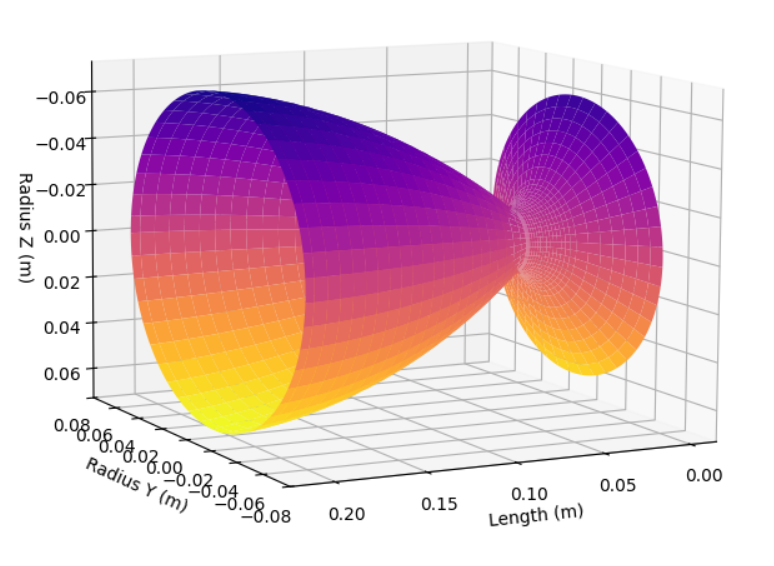
\includegraphics[width=0.84\linewidth]{Images/ex4.png}}{\fbox{\parbox{0.85\linewidth}{\centering Missing figure file: \texttt{ex4.png}}}}
    \caption{Example of three-dimensional nozzle visualization generated by surface revolution.}
    \label{fig:3D_view}
\end{figure}

\begin{figure}[H]
    \centering
    \IfFileExists{Images/ex10.png}{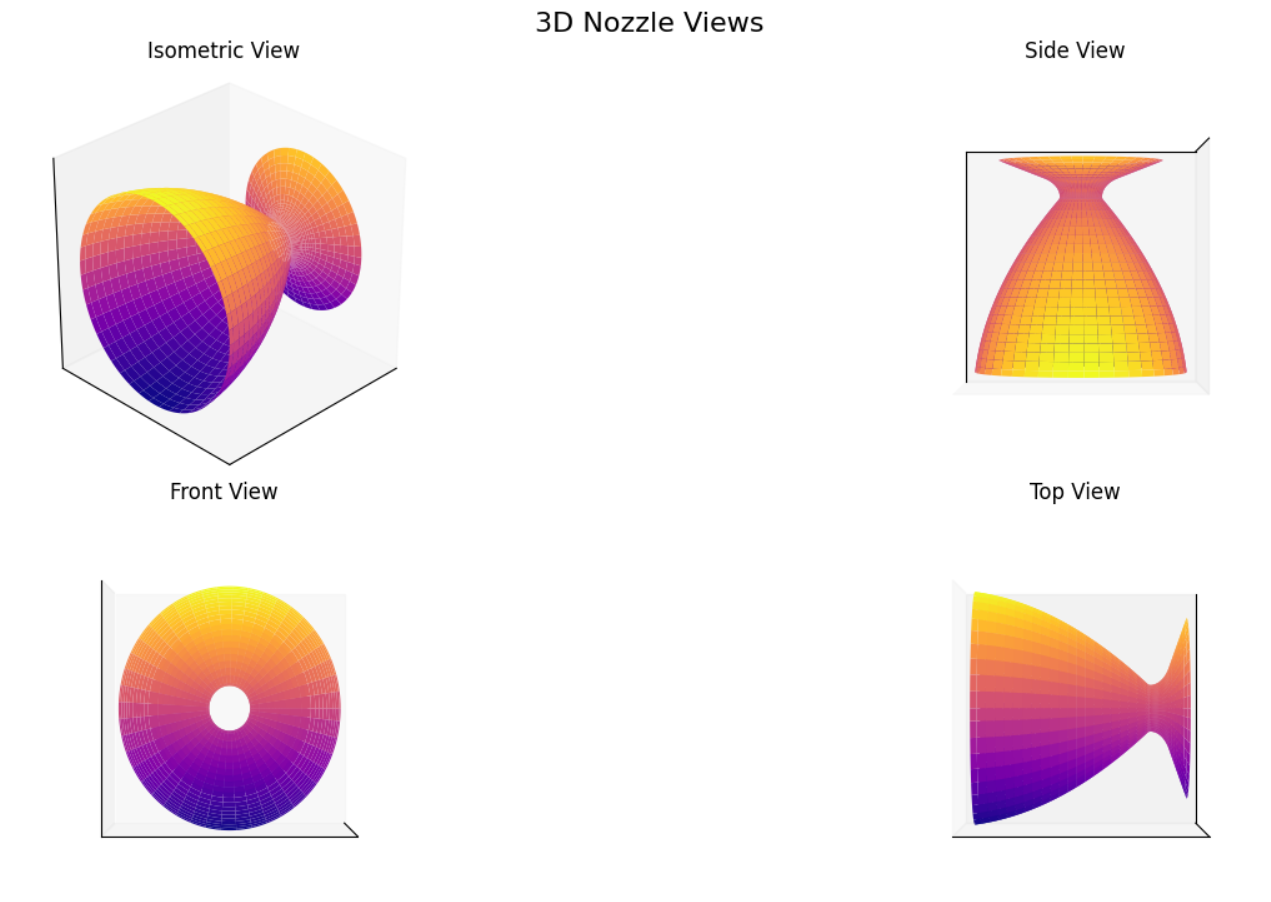
\includegraphics[width=0.88\linewidth]{Images/ex10.png}}{\fbox{\parbox{0.88\linewidth}{\centering Missing figure file: \texttt{ex10.png}}}}
    \caption{Example of multi-view visualization of the generated nozzle geometry.}
    \label{fig:3D_multiview}
\end{figure}

% =========================================================
\subsection{CAD-Oriented Geometry Export and Manufacturing Workflow}
% =========================================================

\subsubsection{CAD-compatible coordinate export}

One of the practical objectives of the simulator is to convert the numerically
generated nozzle contour into a format suitable for computer-aided design (CAD).
The exported coordinates describe the two-dimensional meridional profile of the
nozzle and can be imported into software such as Autodesk Fusion or SolidWorks.

The exported point set is written as
\begin{equation}
    \mathcal{P}
    =
    \left\{
        (x_i,r_i,0)
    \right\}_{i=0}^{N},
\end{equation}
where \(x_i\) is the axial coordinate and \(r_i\) is the corresponding wall
radius. The third coordinate is set to zero because the contour is imported as
a planar curve. Before export, the axial coordinates are translated so that the
first point of the contour is located at \(x=0\), and the coordinates are
converted from metres to millimetres.

The resulting curve represents the internal wall of the nozzle. A
three-dimensional body can subsequently be reconstructed in CAD by defining
the required wall thickness, closing the sketch and revolving the resulting
cross-section around the nozzle axis.

\subsubsection{Point reduction and sketch-conditioning strategy}

The numerical geometry uses a relatively dense point distribution to provide
smooth plots and sufficiently resolved flow, thermal and boundary-layer
profiles. Directly importing this complete point set into CAD, however, may
produce an unnecessarily complex spline. Excessive point density, particularly
near segment junctions, can lead to local oscillations, poor spline conditioning
and difficulties when applying sketch constraints.

\begin{figure}[H]
    \centering
    \begin{subfigure}{0.48\linewidth}
        \centering
        \IfFileExists{Images/ex11.png}
        {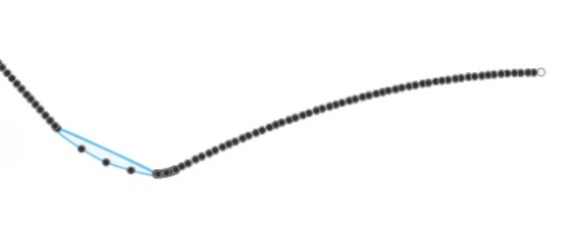
\includegraphics[width=\linewidth]{Images/ex11.png}}
        {\fbox{\parbox{0.95\linewidth}{\centering
        Missing: \texttt{ex11.png}}}}
        \caption{Spline irregularity caused by an excessively dense point set.}
    \end{subfigure}
    \hfill
    \begin{subfigure}{0.48\linewidth}
        \centering
        \IfFileExists{Images/ex12.png}
        {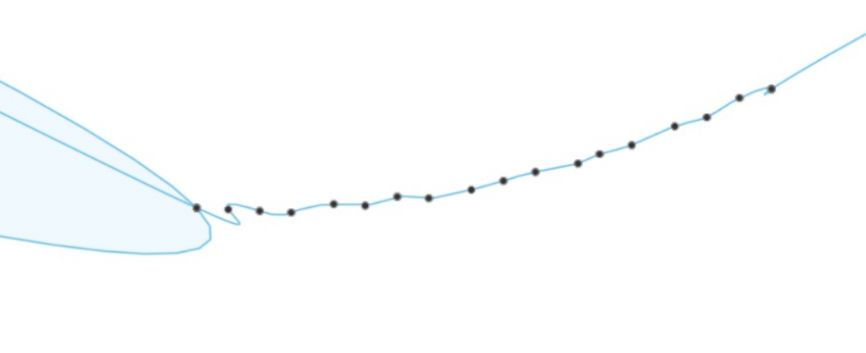
\includegraphics[width=\linewidth]{Images/ex12.png}}
        {\fbox{\parbox{0.95\linewidth}{\centering
        Missing: \texttt{ex12.png}}}}
        \caption{Detailed view of the spline near the throat transition.}
    \end{subfigure}
    \caption{CAD sketch irregularities associated with an unsuitable point
    distribution.}
    \label{fig:cad_irregularity}
\end{figure}


The initial CAD-export implementation therefore included a two-stage
point-conditioning procedure. First, a target of approximately 100 points was
distributed proportionally among the four geometric regions:
\begin{enumerate}
    \item the straight convergent section;
    \item the subsonic throat arc;
    \item the supersonic throat arc;
    \item the parabolic bell contour.
\end{enumerate}
A minimum of two points was retained in each region so that no geometric segment
was omitted. Within each segment, points were selected at approximately uniform
index intervals.

A second sequential filter was then applied to remove clustered points. A
candidate point was retained only when its distance from the previously accepted
point satisfied
\begin{equation}
    d_i
    =
    \sqrt{
        (x_i-x_k)^2+(r_i-r_k)^2
    }
    \geq d_{\min},
\end{equation}
where \(k\) denotes the last accepted point and \(d_{\min}\) is the prescribed
minimum spacing. A value of approximately
\(d_{\min}=1\,\mathrm{mm}\) was used during the CAD-conditioning tests. The
first and final contour points, together with the points defining the main
geometric transitions, should be preserved explicitly to maintain the chamber
inlet, throat and nozzle-exit dimensions.

The current modular implementation exports the complete set of unique geometry
points to \texttt{geometry.csv}. The reduction procedure described above
corresponds to the CAD-conditioning stage developed in the initial version and
can be applied as an additional preprocessing step when a lighter CAD spline is
required.


\subsubsection{CAD reconstruction workflow}

The complete geometry-reconstruction workflow is summarized as follows:
\begin{enumerate}
    \item generate the two-dimensional contour using the geometric model;
    \item translate the axial coordinates so that the contour begins at \(x=0\);
    \item remove duplicate points at the junctions between geometric segments;
    \item reduce and filter the point set when CAD conditioning is required;
    \item convert the coordinates from metres to millimetres;
    \item export the coordinates as a three-column point file;
    \item import the point file into the CAD environment;
    \item create a spline through the imported points;
    \item define the wall thickness by offsetting the internal contour;
    \item close the cross-section and revolve it around the nozzle axis.
\end{enumerate}

%\begin{figure}[H]
%    \centering
%    \IfFileExists{Images/ex13.png}
%    {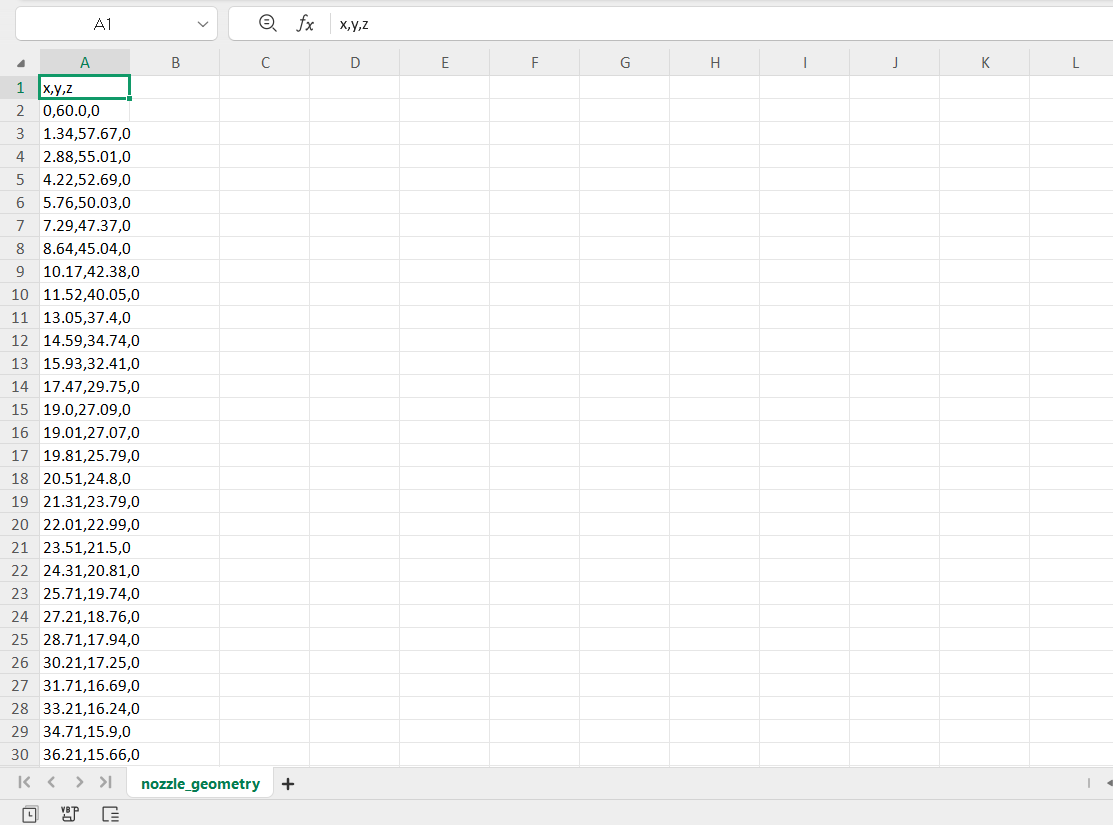
\includegraphics[width=0.85\linewidth]{Images/ex13.png}}
%    {\fbox{\parbox{0.85\linewidth}{\centering
 %   Missing figure file: \texttt{ex13.png}}}}
  %  \caption{Example of the exported nozzle-coordinate file opened in tabular
  %  form.}
  %  \label{fig:csv_output}
%\end{figure}

\begin{figure}[H]
    \centering
    \IfFileExists{Images/ex14.png}
    {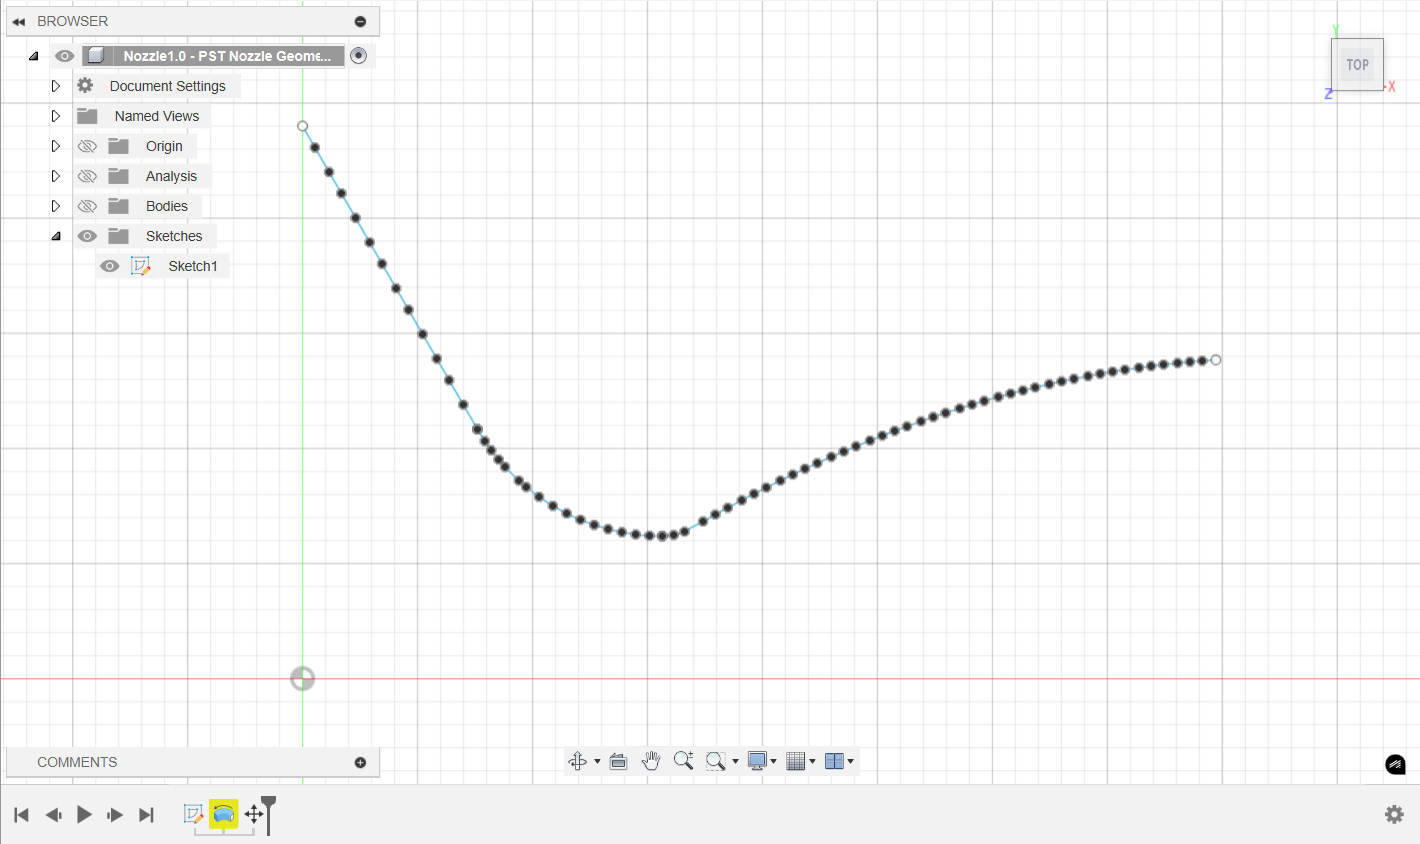
\includegraphics[width=0.78\linewidth]{Images/ex14.png}}
    {\fbox{\parbox{0.78\linewidth}{\centering
    Missing figure file: \texttt{ex14.png}}}}
    \caption{Nozzle contour reconstructed in CAD using the conditioned point
    distribution.}
    \label{fig:cad_sketch}
\end{figure}

\begin{figure}[H]
    \centering
    \begin{subfigure}{0.48\linewidth}
        \centering
        \IfFileExists{Images/ex16.png}
        {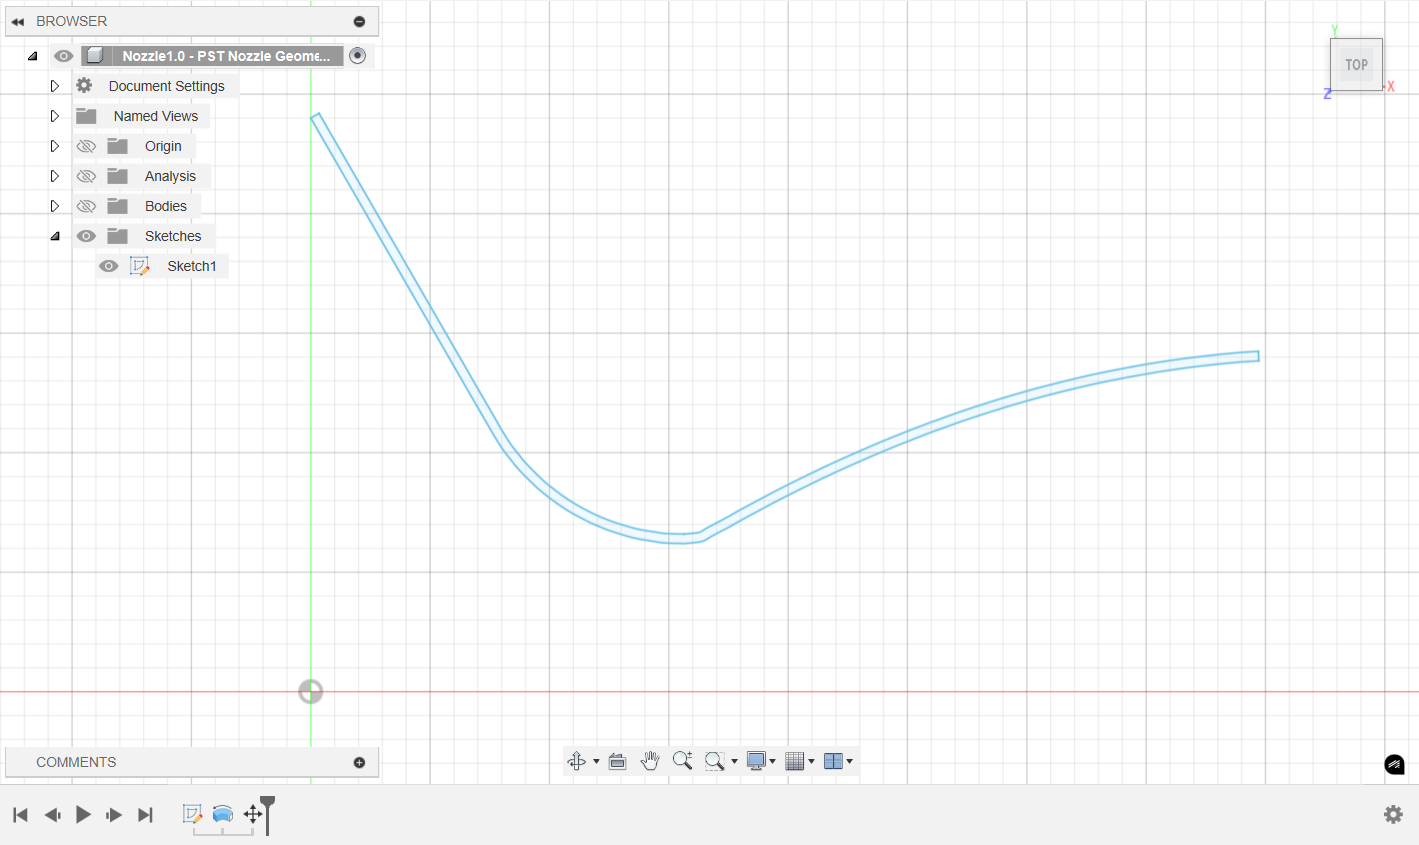
\includegraphics[width=\linewidth]{Images/ex16.png}}
        {\fbox{\parbox{0.95\linewidth}{\centering
        Missing: \texttt{ex16.png}}}}
        \caption{Definition of the nozzle wall thickness.}
    \end{subfigure}
    \hfill
    \begin{subfigure}{0.48\linewidth}
        \centering
        \IfFileExists{Images/ex17.png}
        {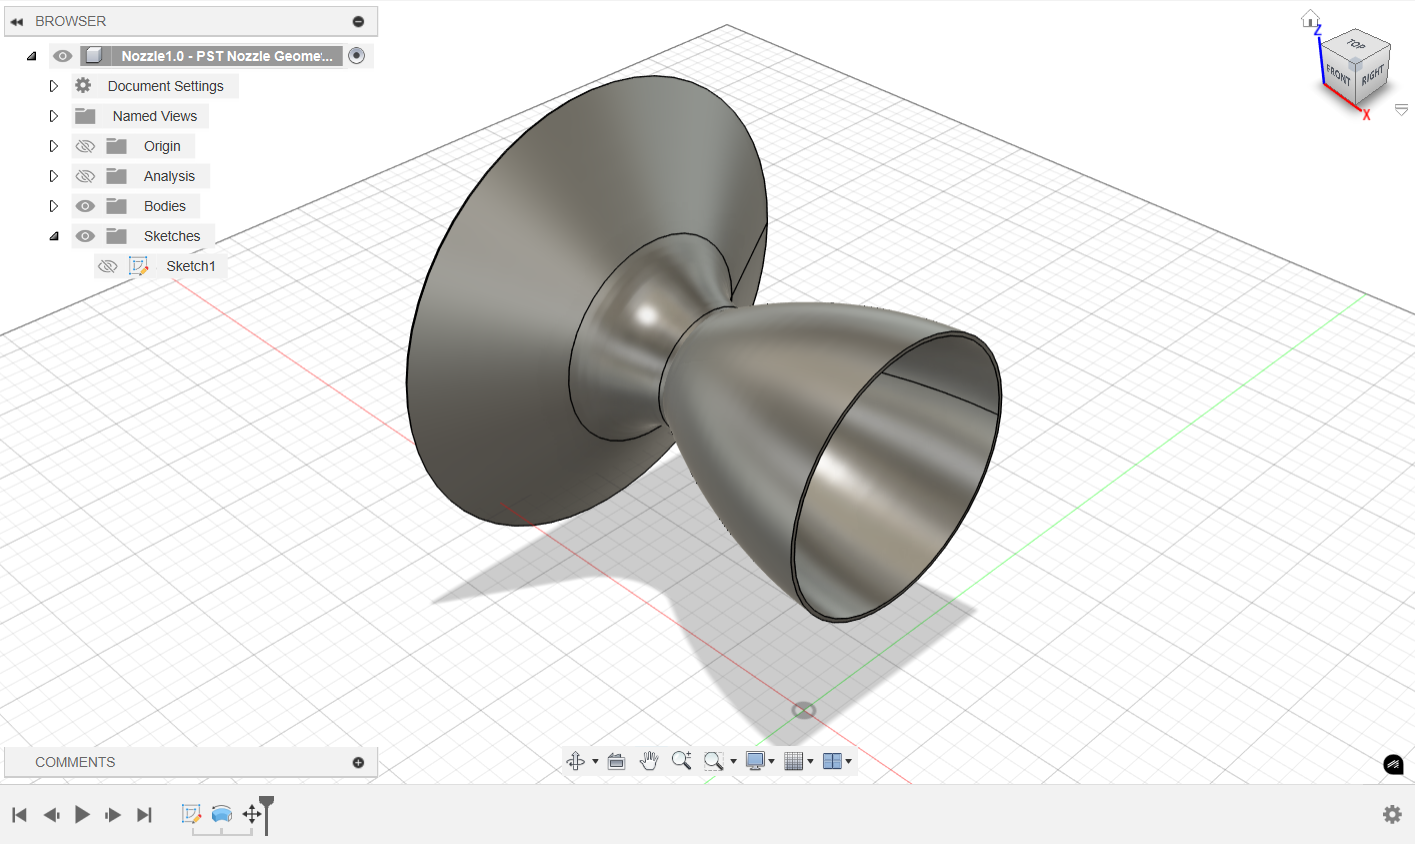
\includegraphics[width=\linewidth]{Images/ex17.png}}
        {\fbox{\parbox{0.95\linewidth}{\centering
        Missing: \texttt{ex17.png}}}}
        \caption{Final axisymmetric nozzle body after revolution.}
    \end{subfigure}
    \caption{CAD operations used to convert the exported meridional contour
    into a manufacturable three-dimensional body.}
    \label{fig:cad_final}
\end{figure}


\newpage
% =========================================================

% =========================================================
\section{Genetic-Algorithm Optimization Framework}
\label{sec:genetic_algorithm}
% =========================================================

\subsection{Optimization problem definition}

The genetic algorithm searches the prescribed design space while retaining the engine
operating point and pre-sizing quantities supplied by the user. The detailed
quasi-one-dimensional, boundary-layer, performance and contour formulations are given
in Sections~\ref{sec:3}--\ref{sec:geometry} and are not repeated here. Within the optimizer, these models are
treated as a coupled candidate-evaluation function

\begin{equation}
\mathcal{S}:\left(\bm{q},\bm{x}_{fixed}\right)
\longrightarrow
C_{F,eff},
\label{eq:coupled_candidate_evaluator}
\end{equation}

where \(\bm{q}\) is the chromosome and \(\bm{x}_{fixed}\) contains the quantities
held constant during one optimization run.

For every candidate, the simulator evaluates the required RocketCEA properties, the
common physical models and the effective thrust coefficient defined in
Eq.~\eqref{eq:effective_thrust_coefficient}. The genetic algorithm therefore operates
on the same physical model used by the simulator rather than on an independent
surrogate.

The Bartz heat-transfer profile is omitted from the repeated fitness calculation
because thermal loading is not part of the current objective. No wall-temperature
input is passed to the evaluator: both boundary-layer closures use the locally derived
adiabatic-wall temperature of Eq.~\eqref{eq:adiabatic_wall_temperature}.

Two evaluation modes are exposed without changing the chromosome or GA operators.
\emph{Quick screening} uses the weak integral closure of
Section~\ref{sec:integral_boundary_layer}; \emph{BLIMP-lite} uses the profile marcher
of Section~\ref{sec:blimp_cebeci_smith}. A solution obtained through Quick screening
is regenerated and reported with BLIMP-lite before it is accepted as the selected
geometry.

% ---------------------------------------------------------
\subsection{Chromosome and fixed quantities}
% ---------------------------------------------------------

\subsubsection{Chromosome definition}

The implemented chromosome contains three real-valued genes:

\begin{equation}
\boxed{
\bm{q}
=
\begin{bmatrix}
\varepsilon & K_b & \theta_{in}
\end{bmatrix}^{T}
},
\label{eq:implemented_chromosome}
\end{equation}

where \(\varepsilon\) is the exit-to-throat area ratio, \(K_b\) is the bell-length
fraction and \(\theta_{in}\) is the initial divergent-wall angle. Their default search
bounds are

\begin{align}
2.0&\leq\varepsilon\leq15.0,
\label{eq:epsilon_gene_bounds}\\
0.60&\leq K_b\leq1.00,
\label{eq:bell_fraction_gene_bounds}\\
20^\circ&\leq\theta_{in}\leq35^\circ.
\label{eq:theta_in_gene_bounds}
\end{align}

All genes are represented as floating-point values. The limits can be changed directly
from the optimization interface.

The exit angle \(\theta_{out}\) is not a gene because it is a derived output of the
contour model. The convergent angle \(\theta_{sub}\) is also excluded from the
chromosome and remains fixed during the search.

\subsubsection{Fixed quantities}

The fixed input vector may be represented as

\begin{equation}
\bm{x}_{fixed}
=
\begin{bmatrix}
p_c & O/F & p_a & r_t & D_c & \alpha & \theta_{sub}
\end{bmatrix}^{T}.
\label{eq:ga_fixed_inputs}
\end{equation}

The default values used by the interface are listed in
Table~\ref{tab:ga_inputs_updated}.

\begin{table}[htbp]
\centering
\caption{Default inputs and their roles during optimization.}
\label{tab:ga_inputs_updated}
\begin{tabular}{llll}
\toprule
Quantity & Symbol & Default value & GA status \\
\midrule
Chamber pressure          & \(p_c\)          & \(30\,\mathrm{bar}\)    & Fixed \\
Mixture ratio             & \(O/F\)          & \(6.5\)                  & Fixed \\
Ambient pressure          & \(p_a\)          & \(1.0\,\mathrm{atm}\)   & Fixed \\
Expansion ratio           & \(\varepsilon\)  & \(5.6\)                  & Optimized \\
Throat radius             & \(r_t\)          & \(0.01728\,\mathrm{m}\) & Fixed \\
Chamber diameter          & \(D_c\)          & \(0.120\,\mathrm{m}\)  & Fixed \\
Reference cone half-angle & \(\alpha\)       & \(15^\circ\)            & Fixed \\
Bell-length fraction      & \(K_b\)          & \(0.80\)                 & Optimized \\
Initial divergent angle   & \(\theta_{in}\)  & \(30^\circ\)            & Optimized \\
Convergent angle          & \(\theta_{sub}\) & \(50^\circ\)            & Fixed \\
\bottomrule
\end{tabular}
\end{table}

The recovery factor is not included because it is derived locally from the
interpolated RocketCEA Prandtl number rather than supplied as an independent input.
Since \(\varepsilon\) is
part of the chromosome, the exit properties returned by RocketCEA are candidate
dependent and cannot be treated as a single common result for the complete population.

% ---------------------------------------------------------
\subsection{Fitness-function definition}
% ---------------------------------------------------------

The scalar objective maximized by the genetic algorithm is the effective ambient
thrust coefficient introduced in Section~\ref{sec:loss_corrected_model}:

\begin{equation}
\boxed{
J(\bm{q})
=
C_{F,eff}(\bm{q})
}.
\label{eq:implemented_ga_fitness}
\end{equation}

Explicitly,

\begin{equation}
J(\bm{q})
=
\eta_{div}(\bm{q})\eta_{BL}(\bm{q})
C_{F,mom}^{CEA}(\bm{q})
+
\varepsilon(\bm{q})
\frac{p_e(\bm{q})-p_a}{p_c}
-C_{F,fric}(\bm{q}).
\label{eq:expanded_ga_fitness}
\end{equation}

The objective is maximized directly, so no sign inversion is required. It contains a
loss-corrected momentum contribution, the signed ambient pressure-thrust contribution
and integrated wall friction. It does not include additional empirical, mass,
manufacturing-cost or thermal-limit penalties.

% ---------------------------------------------------------
\subsection{Candidate validation and constraint handling}
% ---------------------------------------------------------

The gene bounds in Eqs.~\eqref{eq:epsilon_gene_bounds}--%
\eqref{eq:theta_in_gene_bounds} provide the first level of constraint enforcement.
Each generated candidate is then passed to the common simulator validation and to the
models defined in Sections~\ref{sec:3}--\ref{sec:geometry}. The geometric
admissibility conditions are part of the contour model of
Section~\ref{sec:geometry} and are not duplicated here.

A candidate is rejected if the common simulator reports an invalid input, an invalid
contour, a singular numerical system, a non-finite result or a non-positive effective
thrust coefficient. Candidates classified as separated by RocketCEA are also rejected.

Constraint handling uses a death-penalty strategy:

\begin{equation}
J_{GA}(\bm{q})
=
\begin{cases}
C_{F,eff}(\bm{q}),
&\text{valid, finite and attached-flow candidate},\\[1.5mm]
0,
&\text{otherwise}.
\end{cases}
\label{eq:ga_death_penalty}
\end{equation}

There is no continuous penalty proportional to the magnitude of a violation.

% ---------------------------------------------------------
\subsection{Genetic-algorithm configuration}
% ---------------------------------------------------------

The optimizer is implemented using PyGAD \cite{PyGAD}. Its default configuration is summarized in
Table~\ref{tab:ga_configuration_updated}.

\begin{table}[htbp]
\centering
\caption{Default configuration of the implemented genetic algorithm.}
\label{tab:ga_configuration_updated}
\begin{tabular}{ll}
\toprule
Parameter & Implemented value \\
\midrule
Chromosome representation & Three real-valued genes \\
Population size & \(N_p=100\) individuals \\
Maximum generations & \(G_{max}=300\) \\
Mating parents & 20 \\
Parent selection & Tournament selection \\
Crossover & Uniform crossover \\
Crossover probability & \(P_c=0.85\) \\
Mutation & Adaptive mutation \\
Adaptive mutation percentages & \([67\%,34\%]\) \\
Elitism & Best three individuals \\
Saturation limit & 40 generations \\
Default evaluation mode & Four worker processes \\
Repeated-candidate cache & Enabled \\
Saved full solution history & No \\
Explicit random seed & No \\
\bottomrule
\end{tabular}
\end{table}

The settings are user-configurable. The implemented validation requires

\begin{equation}
N_p\geq4,
\qquad
G_{max}\geq1,
\qquad
2\leq N_{parents}\leq N_p.
\label{eq:minimum_ga_settings}
\end{equation}

\subsubsection{Tournament selection}

Tournament selection gives preference to candidates with higher
\(C_{F,eff}\) while preserving stochastic exploration. Candidate parents are sampled
from the current population and the best member of each tournament is selected for
reproduction. With the default settings, 20 parents participate in each generation.

\subsubsection{Uniform crossover}

Uniform crossover constructs each offspring by selecting each gene from either
parent. For example, given

\begin{align}
\bm{q}^{(1)}
&=
\begin{bmatrix}
\varepsilon^{(1)} & K_b^{(1)} & \theta_{in}^{(1)}
\end{bmatrix}^{T},\\
\bm{q}^{(2)}
&=
\begin{bmatrix}
\varepsilon^{(2)} & K_b^{(2)} & \theta_{in}^{(2)}
\end{bmatrix}^{T},
\end{align}

one possible offspring is

\begin{equation}
\bm{q}^{(o)}
=
\begin{bmatrix}
\varepsilon^{(1)} & K_b^{(2)} & \theta_{in}^{(1)}
\end{bmatrix}^{T}.
\label{eq:uniform_crossover_example}
\end{equation}

Crossover is applied with probability \(P_c=0.85\).

\subsubsection{Adaptive mutation}

Adaptive mutation changes the mutation intensity according to candidate fitness. The
configured percentages are

\begin{equation}
\bm{p}_m
=
\begin{bmatrix}
67\% & 34\%
\end{bmatrix}.
\label{eq:adaptive_mutation_percentages}
\end{equation}

Lower-fitness candidates receive the larger mutation percentage, promoting
exploration, while higher-fitness candidates receive the smaller percentage,
promoting local refinement. For the three-gene chromosome, these percentages
correspond approximately to mutating two genes and one gene, respectively. All
mutations remain bounded by the defined gene spaces.

\subsubsection{Elitism}

The best three candidates are transferred directly to the following generation,

\begin{equation}
N_{\mathrm{elite}}=3.
\label{eq:ga_elitism}
\end{equation}

These individuals are preserved without being subjected to crossover or mutation, ensuring that the highest-fitness nozzle geometries already identified by the optimizer are not lost through the stochastic genetic operators. Since only three individuals are retained from a population of 100, elitism preserves the best solutions while leaving most of the population available for continued exploration of the design space. 

% ---------------------------------------------------------
\subsection{Evaluation acceleration}
% ---------------------------------------------------------

The optimizer supports serial, threaded and multiprocess evaluation. The default mode
uses a persistent pool of four worker processes. Each process receives an isolated
RocketCEA working directory, preventing simultaneous Fortran evaluations from using
the same temporary files.

An exact-match fitness cache stores previously evaluated chromosomes. When an
identical chromosome reappears, its stored fitness is reused. The ideal expansion
ratio associated with the fixed values of \(p_c\), \(O/F\) and \(p_a\) is cached
separately because it does not depend on the candidate chromosome.

These measures reduce evaluation time without changing population generation,
selection, crossover, mutation, elitism or stopping logic.

% ---------------------------------------------------------
\subsection{Stopping, cancellation and reported progress}
% ---------------------------------------------------------

The optimization terminates when the first of the following conditions is met:

\begin{enumerate}
    \item the maximum number of generations is reached;
    \item the best fitness does not improve for the selected saturation interval,
    equal to 40 generations by default;
    \item the user requests cancellation through the interface.
\end{enumerate}

Cancellation is checked at the end of each generation. The current generation is
therefore allowed to finish before execution stops.

During execution, the interface displays the completed generation, percentage,
elapsed time, estimated remaining time and generation rate. It also reports the best
\(C_{F,eff}\) and the current chromosome. If no candidate with positive fitness is
found, the optimization is declared unsuccessful.

Otherwise, the returned result is

\begin{equation}
\bm{y}_{GA}
=
\begin{bmatrix}
\varepsilon^* &
K_b^* &
\theta_{in}^* &
\theta_{out}^* &
p_e^* &
C_{F,eff}^* &
N_g
\end{bmatrix}^{T},
\label{eq:ga_output}
\end{equation}

where \(N_g\) is the number of completed generations. The ambient operating-mode
classification is also retained. Because no explicit random seed is assigned,
repeated runs with identical inputs may return slightly different chromosomes.


\subsection{Algorithmic limitations and possible extensions}
% ---------------------------------------------------------

The implemented GA solves a single-objective, single-operating-point problem. It is
stochastic and does not guarantee the global optimum. Its result also depends on the
accuracy and validity range of the coupled simulator used to evaluate each chromosome.

Future algorithmic extensions may include multi-objective optimization, robustness
across several ambient pressures, explicit uncertainty propagation, repeated runs
with controlled random seeds, convergence-statistics reporting and surrogate-assisted
evaluation. Physical or geometric extensions should be introduced in their respective
model sections and then exposed to the GA only through the chromosome, constraints or
candidate-evaluation function.

% ---------------------------------------------------------
\subsection{Optimization workflow}
% ---------------------------------------------------------

Figure~\ref{fig:ga_workflow_updated} summarizes the implemented algorithm without
repeating the internal formulations of the physical simulator.

\begin{figure}[htbp]
\centering
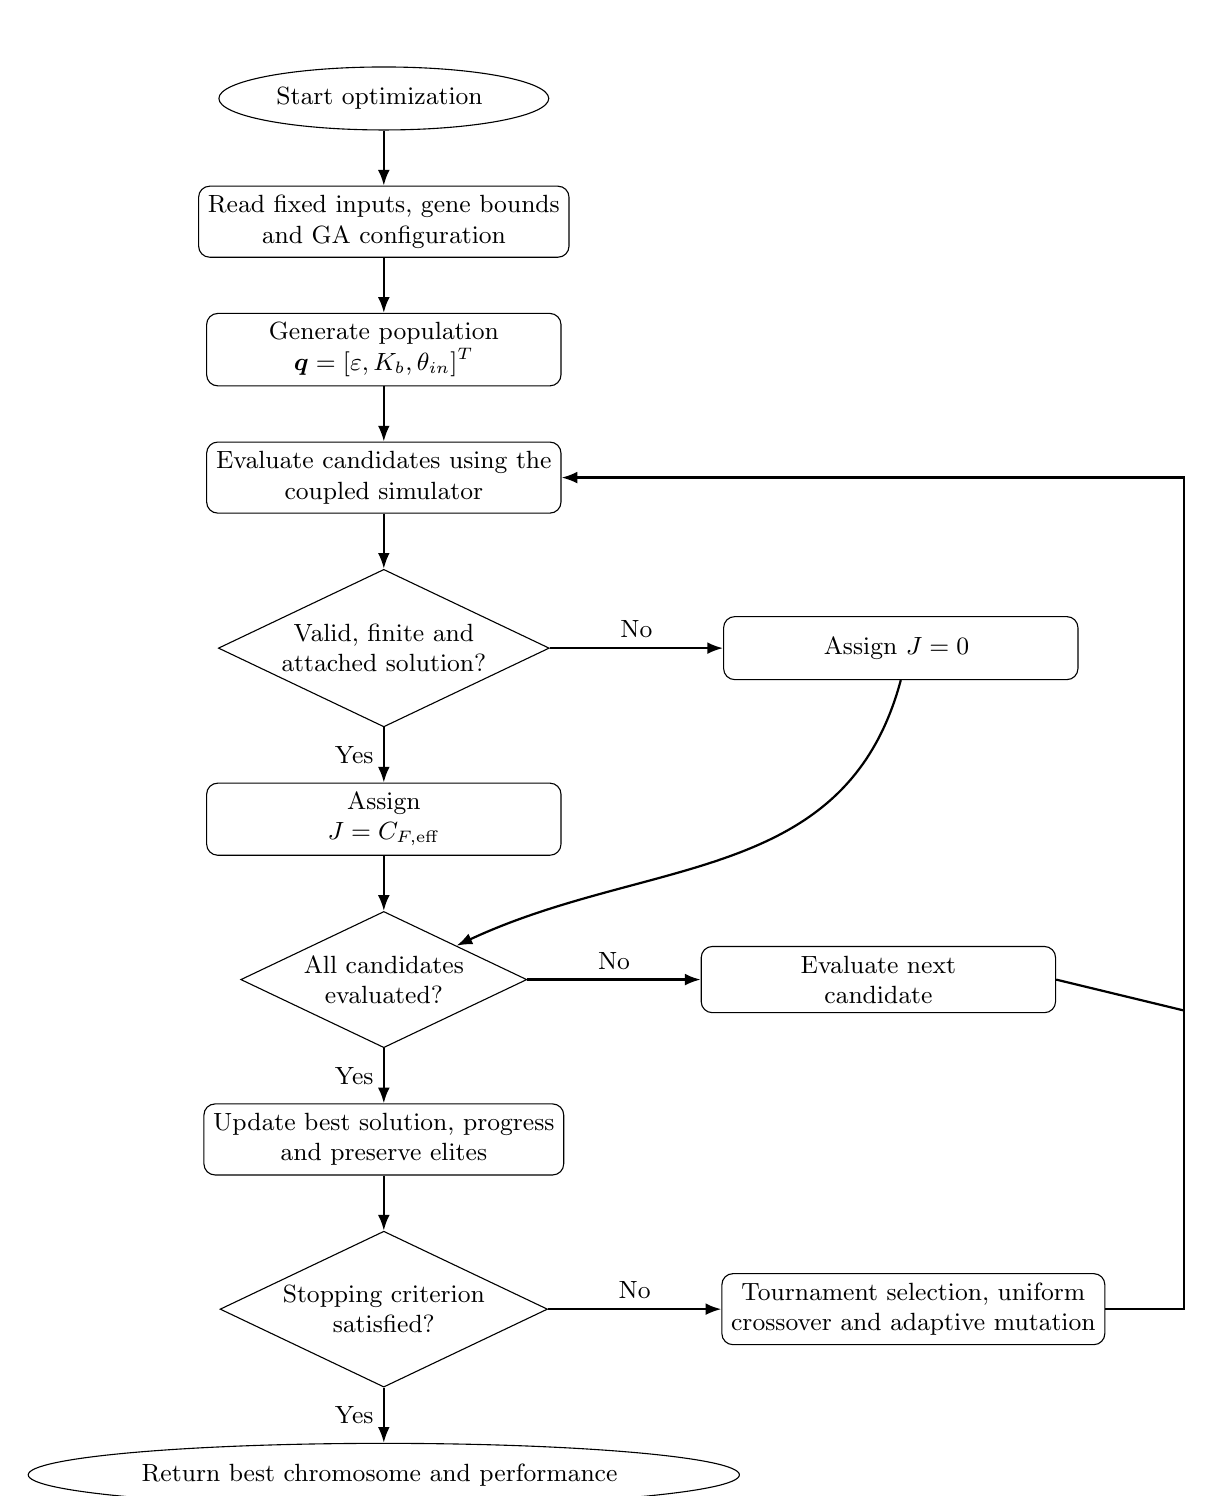
\begin{tikzpicture}[
    node distance=7mm and 18mm,
    every node/.style={font=\small},
    process/.style={
        rectangle,
        rounded corners,
        draw,
        align=center,
        minimum width=45mm,
        minimum height=8mm
    },
    decision/.style={
        diamond,
        draw,
        aspect=2.1,
        align=center,
        inner sep=1.5pt
    },
    terminal/.style={
        ellipse,
        draw,
        align=center,
        minimum width=35mm,
        minimum height=8mm
    },
    arrow/.style={
        -{Latex[length=2mm]},
        thick
    }
]

% =========================================================
% MAIN COLUMN
% =========================================================

\node[terminal] (start) {
Start optimization
};

\node[process, below=of start] (settings) {
Read fixed inputs, gene bounds\\
and GA configuration
};

\node[process, below=of settings] (population) {
Generate population\\
\(\bm{q}=[\varepsilon,K_b,\theta_{in}]^T\)
};

\node[process, below=of population] (evaluate) {
Evaluate candidates using the\\
coupled simulator
};

\node[decision, below=of evaluate] (valid) {
Valid, finite and\\
attached solution?
};

\node[process, below=of valid] (fitness) {
Assign\\
\(J=C_{F,\mathrm{eff}}\)
};

\node[decision, below=of fitness] (all) {
All candidates\\
evaluated?
};

\node[process, below=of all] (progress) {
Update best solution, progress\\
and preserve elites
};

\node[decision, below=of progress] (stop) {
Stopping criterion\\
satisfied?
};

\node[terminal, below=of stop] (output) {
Return best chromosome and performance
};


% =========================================================
% RIGHT-HAND NODES
% =========================================================

\node[process, right=22mm of valid] (zero) {
Assign \(J=0\)
};

\node[process, right=22mm of all] (next) {
Evaluate next\\
candidate
};

\node[process, right=22mm of stop] (reproduce) {
Tournament selection, uniform\\
crossover and adaptive mutation
};


% =========================================================
% MAIN FLOW
% =========================================================

\draw[arrow] (start) -- (settings);
\draw[arrow] (settings) -- (population);
\draw[arrow] (population) -- (evaluate);
\draw[arrow] (evaluate) -- (valid);

% Validity decision
\draw[arrow]
    (valid) -- node[left]{Yes} (fitness);

\draw[arrow]
    (valid) -- node[above]{No} (zero);

\draw[arrow]
    (fitness) -- (all);


% =========================================================
% INVALID CANDIDATE:
% DIRECTLY REJOINS THE "ALL CANDIDATES?" DECISION
% =========================================================

\draw[arrow]
    (zero.south)
    to[out=-105,in=25,looseness=1.05]
    (all.25);


% =========================================================
% CANDIDATE LOOP
% =========================================================

\draw[arrow]
    (all) -- node[left]{Yes} (progress);

\draw[arrow]
    (all) -- node[above]{No} (next);

% Next candidate returns to evaluator
\draw[thick]
    (next.east)
    -- (10.15,-11.58);


% =========================================================
% GENERATION LOOP
% =========================================================

\draw[arrow]
    (progress) -- (stop);

\draw[arrow]
    (stop) -- node[left]{Yes} (output);

\draw[arrow]
    (stop) -- node[above]{No} (reproduce);

% New generation returns to evaluator
\draw[arrow]
    (reproduce.east)
    -- ++(10mm,0)
    |- ([xshift=8mm]evaluate.east)
    -- (evaluate.east);

\end{tikzpicture}

\caption{Flowchart of the implemented genetic-algorithm optimization.}
\label{fig:ga_workflow_updated}
\end{figure}

% ---------------------------------------------------------




\newpage
% =========================================================
% =========================================================
\section{Results and Discussion}
\label{sec:results}

\subsection{Interface}

\begin{figure}[h!]
    \centering
    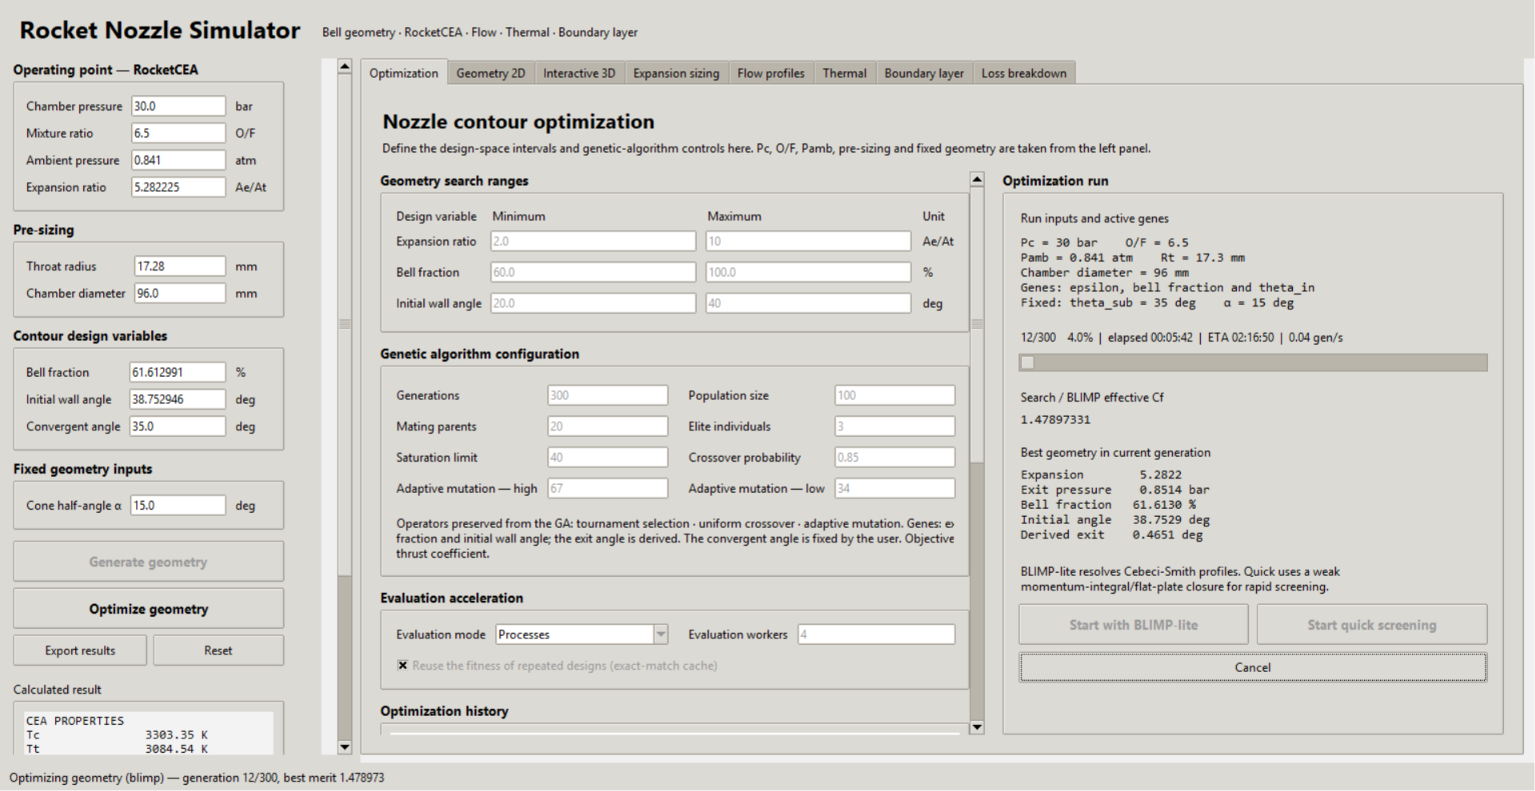
\includegraphics[width=1\linewidth]{int.png}
    \caption{Enter Caption}
    \label{fig:placeholder}
\end{figure}
% =========================================================

\subsection{Evaluation case and data provenance}

The following results use two complete simulator exports retained with the software.
Both cases use the same operating point and are evaluated with the BLIMP-lite closure,
so the comparison changes only the three optimized design variables. The manually
selected baseline is
\begin{equation}
\bm q_0=[5.6,\,0.80,\,30^\circ]^T,
\end{equation}
whereas the best geometry retained from an illustrative GA run is
\begin{equation}
\bm q^*=[5.071819,\,0.600180,\,39.30912^\circ]^T.
\end{equation}
The latter run used a
user-adjusted \(40^\circ\) upper bound for \(\theta_{in}\), rather than the current
\(35^\circ\) default.

\begin{table}[H]
\centering
\caption{Fixed operating-point and pre-sizing inputs used in the comparison.}
\label{tab:result_fixed_inputs}
\begin{tabular}{lll}
\toprule
Quantity & Symbol & Value \\
\midrule
Chamber pressure & \(p_c\) & \(30\,\mathrm{bar}\) \\
Mixture ratio & \(O/F\) & 6.5 \\
Ambient pressure & \(p_a\) & \(0.841\,\mathrm{atm}\) \\
Throat radius & \(r_t\) & \(17.28\,\mathrm{mm}\) \\
Chamber diameter & \(D_c\) & \(120\,\mathrm{mm}\) \\
Convergent angle & \(\theta_{sub}\) & \(50^\circ\) \\
Reference cone half-angle & \(\alpha\) & \(15^\circ\) \\
\bottomrule
\end{tabular}
\end{table}

The CSV files used by the plots below are included with the manuscript. Consequently,
the figures are generated by PGFPlots from the numerical exports rather than inserted
as screenshots. Since the saved run did not retain a random seed or complete population
history, it is reported as a representative optimization result, not as evidence of
statistical GA repeatability or guaranteed global optimality.

\subsection{Geometry selected by the loss-corrected objective}

\begin{table}[H]
\centering
\caption{Baseline and retained GA geometry.}
\label{tab:geometry_comparison}
\begin{tabular}{lrr}
\toprule
Quantity & Baseline & Retained GA candidate \\
\midrule
Expansion ratio, \(\varepsilon\) & 5.6000 & 5.0718 \\
Bell fraction, \(K_b\) & 0.8000 & 0.6002 \\
Initial angle, \(\theta_{in}\) & \(30.000^\circ\) & \(39.309^\circ\) \\
Derived exit angle, \(\theta_{out}\) & \(3.790^\circ\) & \(0.550^\circ\) \\
Total axial length & \(121.886\,\mathrm{mm}\) & \(100.774\,\mathrm{mm}\) \\
\bottomrule
\end{tabular}
\end{table}

\begin{figure}[H]
\centering
\begin{tikzpicture}
\begin{axis}[
    width=0.94\linewidth,
    height=0.48\linewidth,
    xlabel={Axial position [mm]},
    ylabel={Radius [mm]},
    grid=both,
    xmin=0,
    xmax=128,
    ymin=-65,
    ymax=65,
    legend style={at={(0.98,0.98)},anchor=north east,fill=white},
]
\addplot[blue,thick] table[x=x_mm,y=radius_mm,col sep=comma]
    {Images/baseline_geometry.csv};
\addplot[blue,thick,forget plot] table[x=x_mm,y expr=-\thisrow{radius_mm},col sep=comma]
    {Images/baseline_geometry.csv};
\addplot[red!75!black,thick,dashed] table[x=x_mm,y=radius_mm,col sep=comma]
    {Images/optimized_geometry.csv};
\addplot[red!75!black,thick,dashed,forget plot]
    table[x=x_mm,y expr=-\thisrow{radius_mm},col sep=comma]
    {Images/optimized_geometry.csv};
\legend{Baseline,Retained GA candidate}
\end{axis}
\end{tikzpicture}
\caption{Baseline and retained GA contours generated directly from the exported coordinates.}
\label{fig:optimized_geometry_comparison}
\end{figure}

The selected geometry is \(17.32\%\) shorter in total axial length. The higher
initial angle creates stronger early expansion, while the quadratic closure reduces
the derived exit angle to approximately \(0.55^\circ\). This result must be read
together with the model limitations: there is no independent MOC or shock-structure
analysis penalizing rapid internal turning. The admissible bounds therefore remain an
important part of the engineering definition of the search space.

\subsection{Effective thrust coefficient and loss decomposition}

\begin{table}[H]
\centering
\caption{BLIMP-lite performance comparison at the specified ambient pressure.}
\label{tab:performance_comparison}
\begin{tabular}{lrr}
\toprule
Quantity & Baseline & Retained GA candidate \\
\midrule
Exit pressure, \(p_e\) [bar] & 0.7834 & 0.9024 \\
Exit condition & Overexpanded & Underexpanded \\
\(C_{F,mom}^{CEA}\) & 1.511664 & 1.490527 \\
\(\eta_{div}\) & 0.998906 & 0.999977 \\
\(\eta_{BL}\) & 0.996066 & 0.996610 \\
\(C_{F,p}\) & -0.012839 & 0.008504 \\
\(C_{F,fric}\) & 0.017646 & 0.014309 \\
\(C_{F,eff}\) & 1.473586 & 1.479634 \\
Effective thrust [N] & 4147.0 & 4164.0 \\
\bottomrule
\end{tabular}
\end{table}

\begin{figure}[H]
\centering
\begin{tikzpicture}
\begin{axis}[
    ybar,
    bar width=9pt,
    width=0.94\linewidth,
    height=0.50\linewidth,
    ylabel={Modelled decrement, $\Delta C_F$},
    symbolic x coords={Divergence,BL_blockage,Wall_friction,Ambient_mismatch},
    xtick=data,
    xticklabels={Divergence,BL blockage,Wall friction,Ambient mismatch},
    x tick label style={rotate=18,anchor=east},
    ymin=0,
    grid=major,
    legend style={at={(0.5,1.03)},anchor=south,legend columns=2},
]
\addplot[fill=blue!55] table[x=mechanism,y=baseline,col sep=comma]
    {Images/loss_breakdown.csv};
\addplot[fill=red!60] table[x=mechanism,y=optimized,col sep=comma]
    {Images/loss_breakdown.csv};
\legend{Baseline,Retained GA candidate}
\end{axis}
\end{tikzpicture}
\caption{Non-negative loss contributions in thrust-coefficient units. A positive
pressure-thrust contribution is a gain and is therefore excluded from the ambient
mismatch bar.}
\label{fig:loss_breakdown_comparison}
\end{figure}

The effective thrust coefficient increases from 1.473586 to 1.479634, a \(0.41\%\)
improvement for fixed \(p_cA_t\). The retained candidate does not simply choose the
ideal pressure-matched expansion ratio \(\varepsilon_{ideal}=5.2792\). Instead, it
accepts a small positive pressure-thrust contribution and reduces the modelled wall
friction through the shorter contour. In the selected candidate, wall friction
accounts for approximately \(73.8\%\) of the non-negative modelled loss, boundary-layer
blockage for \(26.1\%\), and exit divergence for less than \(0.2\%\). These percentages
describe the implemented closure and must not be interpreted as experimentally
validated loss attribution.

\subsection{Axial flow and boundary-layer response}

\begin{figure}[H]
\centering
\begin{tikzpicture}
\begin{axis}[
    width=0.94\linewidth,
    height=0.46\linewidth,
    xlabel={Axial position [mm]},
    ylabel={Mach number},
    grid=both,
    legend pos=north west,
]
\addplot[blue,thick] table[x expr=1000*\thisrow{x_m},y=mach,col sep=comma]
    {Images/baseline_flow_profile.csv};
\addplot[red!75!black,thick,dashed]
    table[x expr=1000*\thisrow{x_m},y=mach,col sep=comma]
    {Images/optimized_flow_profile.csv};
\legend{Baseline,Retained GA candidate}
\end{axis}
\end{tikzpicture}
\caption{Quasi-one-dimensional Mach reconstruction for the two geometries.}
\label{fig:mach_comparison}
\end{figure}

\begin{figure}[H]
\centering
\begin{tikzpicture}
\begin{axis}[
    width=0.94\linewidth,
    height=0.46\linewidth,
    xlabel={Axial position [mm]},
    ylabel={Displacement thickness [mm]},
    grid=both,
    legend pos=north west,
]
\addplot[blue,thick]
    table[x expr=1000*\thisrow{x_m},y expr=1000*\thisrow{delta_star_m},col sep=comma]
    {Images/baseline_boundary_layer.csv};
\addplot[red!75!black,thick,dashed]
    table[x expr=1000*\thisrow{x_m},y expr=1000*\thisrow{delta_star_m},col sep=comma]
    {Images/optimized_boundary_layer.csv};
\legend{Baseline,Retained GA candidate}
\end{axis}
\end{tikzpicture}
\caption{BLIMP-lite compressible displacement-thickness distributions.}
\label{fig:displacement_thickness_comparison}
\end{figure}

The exported profiles remain finite and continuous across all four geometric
segments. The comparison also illustrates why \(\eta_{BL}\) and \(C_{F,fric}\) are
kept separate: the former represents the effective-area velocity correction, whereas
the latter is obtained by integrating the resolved wall shear. A publication-level
assessment of optimizer robustness will additionally require repeated seeded runs,
population convergence statistics and validation of the retained candidate with an
independent higher-fidelity method.

\newpage
% =========================================================
\section{Limitations and Future Work}
% =========================================================

The present framework is a reduced-order, single-operating-point preliminary design
tool. Its principal limitations are:
\begin{itemize}
    \item no method-of-characteristics or multidimensional wave analysis of the
    parameterized contour;
    \item no CFD-resolved shocks, separation or shock--boundary-layer interaction;
    \item no finite-rate chemistry or station-by-station equilibrium/frozen transition;
    \item interpolated RocketCEA properties used with local perfect-gas relations;
    \item fully turbulent, attached-flow BLIMP-lite and Quick closures with an
    engineering inlet boundary-layer initialization;
    \item an adiabatic wall with no conjugate thermal, coolant, ablative or structural model;
    \item no experimental calibration of \(\eta_{div}\), \(\eta_{BL}\) or
    \(C_{F,fric}\);
    \item a single objective and a single ambient pressure per optimization run.
\end{itemize}

Future work should prioritize:
\begin{enumerate}
    \item repeated seeded GA runs with convergence and uncertainty statistics;
    \item comparison of Quick and BLIMP-lite rankings over a common design sample;
    \item independent validation of geometry continuity, boundary-layer quantities and
    thrust loss against published experiments or mesh-refined RANS/CFD;
    \item trajectory-weighted or multi-point optimization across ambient pressure;
    \item thermal and structural constraints for manufacturable designs;
    \item optional MOC analysis of selected parametric contours as a validation layer,
    without replacing the present geometry family;
    \item comparison between conical, Rao TOP and optimized parametric bell contours.
\end{enumerate}

The lack of a separate empirical turning penalty is deliberate. Rapid turning is
currently controlled through geometric admissibility and bounded values of
\(\theta_{in}\), while its multidimensional wave consequences remain outside the
validity of the quasi-one-dimensional closure. Such effects should be introduced only
through a defensible MOC, CFD or experimental analysis rather than an uncalibrated
coefficient.

\newpage
% =========================================================
\section{Conclusion}
% =========================================================

This work presents an implemented preliminary-design framework for a single bell
nozzle. A continuous piecewise contour composed of a straight convergent, circular
subsonic and supersonic throat arcs, and a quadratic divergent section supports
two-dimensional plotting, axisymmetric three-dimensional visualization, CAD export
and quasi-one-dimensional flow reconstruction. The throat radius is retained from
engine pre-sizing, while the exit radius follows from the expansion ratio.

The genetic algorithm varies three real-valued design variables:
\(\varepsilon\), \(K_b\) and \(\theta_{in}\). The convergent angle and reference
cone half-angle remain user-selected fixed inputs, and the exit wall angle is derived
from the resulting quadratic contour. The optimized objective is the effective
ambient thrust coefficient, combining RocketCEA momentum performance, exit divergence,
compressible boundary-layer blockage, signed pressure thrust and integrated wall
friction. No independent curvature or empirical turning efficiency is used.

Two viscous evaluation levels provide a practical cost--fidelity trade-off. Quick
screening uses a weak momentum-integral closure, whereas BLIMP-lite resolves a
wall-normal velocity profile with a Cebeci--Smith eddy-viscosity model and is used for
final reporting. Both assume an attached, fully turbulent and adiabatic wall; hence
\(T_w=T_{aw}\) and the present model does not predict non-zero wall heat flux.

For the representative saved run, the selected geometry reduced total length by
\(17.32\%\) and increased \(C_{F,eff}\) by \(0.41\%\) relative to the baseline.
This result demonstrates the coupled workflow rather than final nozzle qualification.
The framework is therefore suitable for transparent preliminary comparison and
design-space exploration, provided that final candidates are validated using
independent higher-fidelity analysis and experimental evidence.


% ========================================================
\begin{thebibliography}{99}

\bibitem{SuttonBiblarz}
G. P. Sutton and O. Biblarz, \textit{Rocket Propulsion Elements}, 9th ed., Wiley, 2017.

\bibitem{NASA_CEA}
S. Gordon and B. J. McBride, \textit{Computer Program for Calculation of Complex Chemical Equilibrium Compositions and Applications}, NASA Reference Publication 1311, 1994.

\bibitem{RocketCEA}
C. E. DeLong, \textit{RocketCEA Documentation}, Python interface for NASA CEA.

\bibitem{Anderson}
J. D. Anderson, \textit{Modern Compressible Flow: With Historical Perspective}, McGraw-Hill.

\bibitem{BLIMPJ}
R. M. Evans, \textit{BLIMP-J User's Manual: Boundary Layer Integral Matrix Procedure for JANNAF Rocket Engine Performance Evaluation Methodology}, AEROTHERM-UM-75-64, NASA-CR-144046, 1975.

\bibitem{BLIMPVerification}
W. S. Bonnett and R. M. Evans, \textit{Boundary Layer Integral Matrix Procedure: Verification of Models}, AEROTHERM-77-239, NASA-CR-150271, 1977.

\bibitem{CebeciSmith}
T. Cebeci and A. M. O. Smith, \textit{Analysis of Turbulent Boundary Layers}, Academic Press, 1974.

\bibitem{Walz}
A. Walz, \textit{Boundary Layers of Flow and Temperature}, MIT Press, 1969.

\bibitem{Bartz}
D. R. Bartz, ``A Simple Equation for Rapid Estimation of Rocket Nozzle Convective Heat Transfer Coefficients,'' \textit{Jet Propulsion}, vol. 27, pp. 49--51, 1957.

\bibitem{PyGAD}
A. F. Gad, ``PyGAD: An Intuitive Genetic Algorithm Python Library,'' \textit{Multimedia Tools and Applications}, 2023.

\end{thebibliography}

\end{document}
